%%%%%%%%%%%%%%%%%%%%%%%%%%%%%%%%%%%%%%%%%%%%%%%%%%%%%%%%%%%%%%%%%
%
% Project     : Turnverein App
% Title       : 
% File        : doc.tex Rev. 00
% Date        : 07.07.14
% Author      : Raffael Santschi
%
%%%%%%%%%%%%%%%%%%%%%%%%%%%%%%%%%%%%%%%%%%%%%%%%%%%%%%%%%%%%%%%%%

%%%%%%%%%%%%%%%%%%%%%%%%%%%%%%%%%%%%%%%%%%%%%%%%%%%%%%%%%%%%%%%%%
%  _____   ____  _____                                          %
% |_   _| /  __||  __ \    Institute of Computitional Physics   %
%   | |  |  /   | |__) |   Zuercher Hochschule Winterthur       %
%   | |  | (    |  ___/    (University of Applied Sciences)     %
%  _| |_ |  \__ | |        8401 Winterthur, Switzerland         %
% |_____| \____||_|                                             %
%%%%%%%%%%%%%%%%%%%%%%%%%%%%%%%%%%%%%%%%%%%%%%%%%%%%%%%%%%%%%%%%%
%
% Project     : LaTeX doc Vorlage für Windows ProTeXt mit TexMakerX
% Title       : 
% File        : header.tex Rev. 00
% Date        : 23.4.12
% Author      : Remo Ritzmann
% Feedback bitte an Email: remo.ritzmann@pfunzle.ch
%
%%%%%%%%%%%%%%%%%%%%%%%%%%%%%%%%%%%%%%%%%%%%%%%%%%%%%%%%%%%%%%%%%

\documentclass[twoside,10pt,parskip=half,ngerman,pointlessnumbers,openright]{scrreprt}

%***********************************************************************
% include some libs
%***********************************************************************
\usepackage[utf8]{inputenc}
\usepackage{listings}
\usepackage{color}
\usepackage{fancyhdr}
\usepackage{rotating}
\usepackage{titlesec}
\usepackage{mathptmx}
% \usepackage{helvet}
\usepackage[scaled]{uarial}
\renewcommand*\familydefault{\sfdefault} %% Only if the base font of the document is to be sans serif
\usepackage[T1]{fontenc}
\usepackage{ngerman}
\usepackage{textcomp}
\usepackage[squaren]{SIunits}
\usepackage{graphicx}
\usepackage{subfigure}
\usepackage{url}
\usepackage{geometry}
\usepackage[absolute]{textpos}
\usepackage{makeidx}
\usepackage{colortbl}
\usepackage{pdflscape}
\usepackage{pdfpages}
\usepackage{tabularx}
\usepackage{lmodern}
\usepackage{longtable}
\usepackage{array}
\usepackage{float}
\usepackage{scrhack}
\usepackage[plainpages=false]{hyperref}
\usepackage{wallpaper} %\ThisTileWallPaper{}
\usepackage[super,square]{natbib} %für BibTeX Literaturverzeichnis
\usepackage{amsmath}
\usepackage[section]{placeins}
\usepackage{booktabs}




%***********************************************************************
% various styles
%***********************************************************************	

%create index
\makeindex

%define pagestyle
\pagestyle{fancy}

%use sans-serif font 
%\renewcommand{\familydefault}{\sfdefault}

%define page margin
\geometry{a4paper, top=30mm, left=30mm, right=30mm, bottom=30mm,headsep=10mm,footskip=10mm}

%textpos parameter
\setlength{\TPHorizModule}{30mm}
\setlength{\TPVertModule}{\TPHorizModule}
\textblockorigin{10mm}{10mm} % start everything near the top-left corner
\setlength{\parindent}{0pt}

%horizontal lines for titlepage 
\newcommand{\HRule}{\rule{\linewidth}{0.5mm}}

%reference to source items inlc source number
\newcommand{\srcref}[1]{\nameref{src:#1} \cite{#1}}

%header / footer 
\renewcommand{\headrulewidth}{0.3pt}
\renewcommand{\footrulewidth}{0.3pt}

\fancyhead[LO,RE]{} %clear headings for contents 
\fancyhead[RO,LE]{\nouppercase{\rightmark}} %right odd pages and left even pages
\fancyhead[LO,RE]{\MakeUppercase{\leftmark}} %left odd pages and right even pages
\fancyfoot[LE,RO]{\thepage} %page numbering
\fancyfoot[C]{} %clear centered page numbering 

%define some colors
\definecolor{gray}{rgb}{0.95,0.95,0.95}
\definecolor{darkgray}{rgb}{0.4,0.4,0.4}
%listing colors
\definecolor{lgray}{RGB}{250,250,250}
\definecolor{lgreen}{RGB}{63,127,95}
\definecolor{lred}{RGB}{127,0,85}
\definecolor{lblue}{RGB}{42,0,255}

% footnote layout optimization
\deffootnote[1.25em]{1.25em}{1.25em}{\textsuperscript{\normalfont\thefootnotemark\,}}

%***********************************************************************
% listing
%***********************************************************************

\lstset{		
		basicstyle=\small\ttfamily,
		frame=single,
		numbers=left,	
		numberstyle=\tiny,
		%firstnumber=auto,
		numberblanklines=true,
		captionpos=b,
		extendedchars=true,
		float=ht,
		showtabs=false,
		tabsize=2,
		showspaces=false,
		showstringspaces=false,
		breaklines=true,
		%prebreak=\Righttorque,
		backgroundcolor=\color{lgray},
		keywordstyle=\color{lred}\bfseries, 
		commentstyle=\color{lgreen}\ttfamily,
%		morekeywords={printstr, printhexln},
		stringstyle=\color{lblue},
		xleftmargin=0.5cm,
		xrightmargin=0.5cm
}

\lstloadlanguages{C++}

% Trennmuster
\hyphenation{Back-end}

%\lstdefinelanguage{xc}{
%     keywords={printstr, printhexln, attributes, class, classend, do, empty, endif, endwhile, fail, function, functionend, if, implements, in, inherit, inout, not, of, operations, out, return, set, then, types, while, use},
%     keywordstyle=\color{lred}\bfseries,
%     ndkeywords={},
%     ndkeywordstyle=\color{yellow}\bfseries,
%     identifierstyle=\color{black},
%     sensitive=false,
%     comment=[l]{//},
%     commentstyle=\color{lgreen}\ttfamily,
%     string=[l]{"},
%     stringstyle=\color{lblue}\ttfamily
%  }



\begin{document}
%\bibliographystyle{plainnat}
\bibliographystyle{alphadin}


\title{PA/BA Latex Vorlage}
\author{Raffael Santschi}


%%%%%%%%%%%%%%%%%%%%%%%%%%%%%%%%%%%%%%%%%%%%%%%%%%%%%%%%%%%%%%%%%
%
% Project     : Turnverein App
% Title       : 
% File        : titlepage.tex Rev. 00
% Date        : 07.07.14
% Author      : Raffael Santschi
%
%%%%%%%%%%%%%%%%%%%%%%%%%%%%%%%%%%%%%%%%%%%%%%%%%%%%%%%%%%%%%%%%%

\begin{titlepage}

% Logo
\ThisTileWallPaper{\paperwidth}{\paperheight}{images/logos/SoE.pdf} % {images/logos/*.pdf}
% Wählen Sie aus folenden pdf Files: ICP, IDP, IEFE, IMES, IMPE, IMS, INE, InES, InIT, KSR, SoE, ZAMP, ZAV, ZIL, ZPP, ZSN

\begin{minipage}[b]{0.117\textwidth}
\hskip 0.05cm
\end{minipage}
\begin{minipage}[b]{0.91\textwidth}
\begin{tiny}.\end{tiny}\vskip 2.8cm
	{\huge
	
	% Projekt Name
	\textbf{\underline{Semesterarbeit Informatik}}\\
	
	% Projekt Titel
	
	Entwicklung einer interaktiven Mobile App mit Kommunikation via RESTful-Webservice zum Backend
	\vskip 0.5cm}
	
	\begin{minipage}[b]{0.27\textwidth}
	\hrule\vskip 0.5cm
		\textbf{Autor}\\
		\\
		\\
		\\
	\end{minipage}
	\begin{minipage}[b]{0.03\textwidth}
	\hskip 0.5cm
	\end{minipage}
	\begin{minipage}[b]{0.7\textwidth}
	\hrule\vskip 0.5cm
		Raffael Santschi\\
		santsraf@students.zhaw.ch\\
		Student im 7. Semester\\
		\\
	\end{minipage}
	
	\begin{minipage}[b]{0.27\textwidth}
	\hrule\vskip 0.5cm
		\textbf{Hauptbetreuung}\\
		\\
		\\
	\end{minipage}
	\begin{minipage}[b]{0.03\textwidth}
	\hskip 0.5cm
	\end{minipage}
	\begin{minipage}[b]{0.7\textwidth}
	\hrule\vskip 0.5cm
		Beat Seeliger\\
		xsel@zhaw.ch\\
		\\
	\end{minipage}
	
	\begin{minipage}[b]{0.27\textwidth}
	\hrule\vskip 0.5cm
		\textbf{Abgabedatum}
	\end{minipage}
	\begin{minipage}[b]{0.03\textwidth}
	\hskip 0.5cm
	\end{minipage}
	\begin{minipage}[b]{0.7\textwidth}
	\hrule\vskip 0.5cm
		01.10.2014
	\end{minipage}

\end{minipage}
\vskip 0.5cm


\end{titlepage}

\setcounter{page}{1}
%%%%%%%%%%%%%%%%%%%%%%%%%%%%%%%%%%%%%%%%%%%%%%%%%%%%%%%%%%%%%%%%%%
%  _____   ____  _____                                          %
% |_   _| /  __||  __ \    Institute of Computitional Physics   %
%   | |  |  /   | |__) |   Zuercher Hochschule Winterthur       %
%   | |  | (    |  ___/    (University of Applied Sciences)     %
%  _| |_ |  \__ | |        8401 Winterthur, Switzerland         %
% |_____| \____||_|                                             %
%%%%%%%%%%%%%%%%%%%%%%%%%%%%%%%%%%%%%%%%%%%%%%%%%%%%%%%%%%%%%%%%%
%
% Project     : LaTeX doc Vorlage für Windows ProTeXt mit TexMakerX
% Title       : 
% File        : Kontakt.tex Rev. 00
% Date        : 23.4.12
% Author      : Remo Ritzmann
% Feedback bitte an Email: remo.ritzmann@pfunzle.ch
%
%%%%%%%%%%%%%%%%%%%%%%%%%%%%%%%%%%%%%%%%%%%%%%%%%%%%%%%%%%%%%%%%%

\textbf{Kontakte}


\textbf{Vorlagen Ersteller} \\
M.Sc. Engineering ZHAW Remo Ritzmann \\
Wissenschaftliche Assistent Optoelectronic Research Laboratory\\
School of Engineering\\
Technikumstrasse 9, TL419\\
CH-8408 Winterthur

Phone: +41 (0)52 534 48 62\\
Zentrale: +41 (0)58 934 73 06\\
Mobile: +41 (0)79 830 17 35\\
E-Mail: remo.ritzmann@zhaw.ch\\
E-Mail Privat: remo.ritzmann@pfunzle.ch\\
Homepage: \url{http://www.icp.zhaw.ch}\vskip 15pt

%%%%%%%%%%%%%%%%%%%%%%%%%%%%%%%%%%%%%%%%%%%%%%%%%%%%%%%%%%%%%%%%%
%
% Project     : Turnverein App
% Title       : 
% File        : abstract.tex Rev. 00
% Date        : 07.07.14
% Author      : Raffael Santschi
%
%%%%%%%%%%%%%%%%%%%%%%%%%%%%%%%%%%%%%%%%%%%%%%%%%%%%%%%%%%%%%%%%%

\thispagestyle{empty}



\newpage
\thispagestyle{empty}
\chapter*{Abstract}\label{abstract}
Der Turnverein Grafstal hat etwa 50 aktive Mitglieder und engagiert sich in der Leichtathletik. Der Verein verwaltet seit gut zwei Jahren seine Veranstaltungen und die dazugehörigen Anmeldungen auf einer Homepage. Im Zusammenhang mit den Feierlichkeiten des 125-jährigen Jubiläums wünschte er sich eine App.\\

Diese Semesterarbeit befasst sich mit der Erstellungen dieser App, die auf verschiedene Plattformen verfügbar sein sollte. Des Weiteren war eine Fahrgemeinschaftsverwaltung für die Entlastung des Chats und Anmeldefunktionalität für die Veranstaltungen gewünscht.\\

Im Rahmen der Arbeit wurden die \glossarmark{Stakeholder} evaluiert und mit diesen eine Anforderungsanalyse durchgeführt. Die Analyse brachte die wichtigsten Anforderungen an die App hervor, des Weiteren wurden \glossarmark{Mockups} für die entstehenden Ansichten erstellt. Durch eine Nutzwertanalyse wurde die geeignete Architektur für die App ermittelt. Ausgehend von dieser Architektur wurde die App dann entwickelt.\\

Bei der Ist-Analyse des Backends fiel auf, dass dieses keine klare Strutkur aufwies, deshalb wurde ein \glossarmark{Refactoring} angedacht und durchgeführt. Im Anschluss wurde das Backend um ein \glossarmark{RESTful} \glossarmark{API} erweitert. Die resultierende App wurde mit dem Framework Phonegap und jQuery Mobile für die Plattformen Android und iOS erstellt. Die Daten für die verschiedenen Seiten wurden per \glossarmark{Ajax}-Request über das \glossarmark{RESTful} \glossarmark{API} geladen. Darüber hinaus wurden die zwei Push-Nachrichten Dienste von Android und iOS in die App eingebunden. Eine Woche nach der Bereitstellung der App konnten bereits 50 Downloads verzeichnet werden. Die Mitglieder verwenden die Fahrgemeinschaftsverwaltung, der Chat wurde entlastet und die Anmeldungen an Veranstaltungen werden vermehrt über die App gemacht.

\chapter*{Vorwort}\label{vorwort}
Apps sind aus der heutigen Zeit nicht mehr weg zu denken. Sie schaffen neue Möglichkeiten und erleichtern unser Leben. Sie sind jedoch auch mit neuen Pflichten verbunden. Es wird von einem erwartet, dass man ständig online und erreichbar ist und in der heutigen Zeit wird von grösseren Dienstleistungsunternehmen erwartet, ein App bereitzustellen, zumal inzwischen das Smartphone für unter 40-jährige wichtiger ist als der Fernseher (siehe \cite{digitalisierungsbericht2014}). Am letzten Apple Event (siehe \cite{apple_event_sept_2014}) wurde berichtet, dass bereits über 1.3 Millonen Apps im App Store vorhanden sind. Mich faszinieren Apps schon eine ganze Weile. Dies war mit einer der Gründe, warum ich an einem zweiwöchigen Austauschprojekt an der Grand Valley State University in Michigan teilnahm. Das Thema in diesem Austauschprogramm war die Mobile App Entwicklung.\\

Die App für den Turnverein war für mich eine gute Gelegenheit für eine Semesterarbeit. Das Projekt hat mich von Anfang an gefesselt und war auch in der vorgegebenen Zeit umsetzbar. Während und nach dem Aufenthalt in Michigan hatte ich bereits mit einem Entwurf einer Native App angefangen, somit wusste ich in etwa, was auf mich zu kam.\\

Mein Dank gebührt meinen Kommilitonen, allen vorweg Roman Lickel, Max Schrimpf und Dominic Schlegel, für die Hilfe in technischen Fragen und Tipps zur Dokumentation. Ganz besonderes möchte ich mich bei Beat Seeliger für die gute Betreuung und seine konstruktive Kritik und bei meinen Korrekturlesern bedanken.

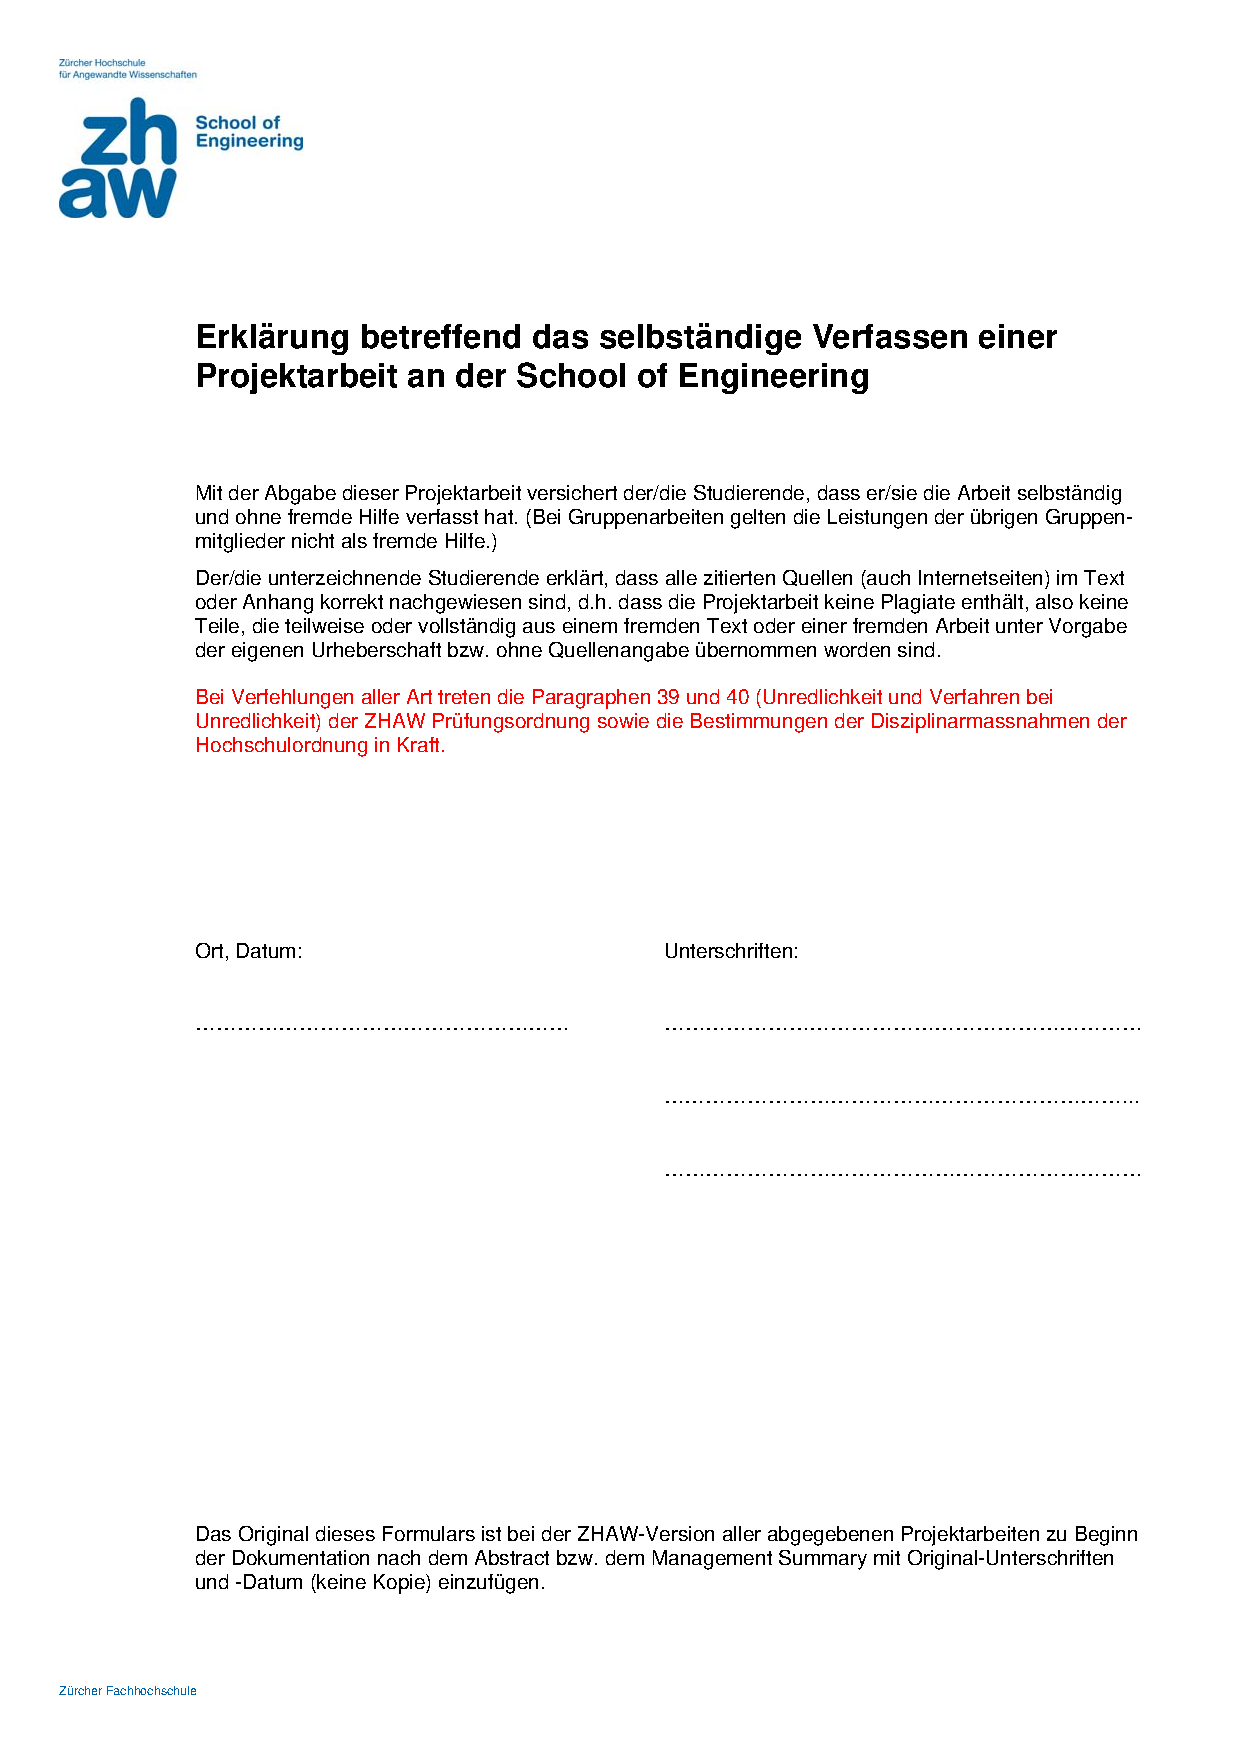
\includepdf{images/Erklaerung_PA.pdf} % Entsprechendes auskommentieren
% \newpage

%Inhaltsverzeichnis
\tableofcontents
\newpage



%\textbf{}
%\setcounter{page}{1}
%\pagenumbering{arabic}

%%%%%%%%%%%%%%%%%%%%%%%%%%%%%%%%%%%%%%%%%%%%%%%%%%%%%%%%%%%%%%%%%%
%  _____   ____  _____                                          %
% |_   _| /  __||  __ \    Institute of Computitional Physics   %
%   | |  |  /   | |__) |   Zuercher Hochschule Winterthur       %
%   | |  | (    |  ___/    (University of Applied Sciences)     %
%  _| |_ |  \__ | |        8401 Winterthur, Switzerland         %
% |_____| \____||_|                                             %
%%%%%%%%%%%%%%%%%%%%%%%%%%%%%%%%%%%%%%%%%%%%%%%%%%%%%%%%%%%%%%%%%
%
% Project     : LaTeX doc Vorlage für Windows ProTeXt mit TexMakerX
% Title       : 
% File        : header.tex Rev. 01
% Date        : 05.06.2012
% Author      : Remo Ritzmann
% Feedback bitte an Email: remo.ritzmann@pfunzle.ch
%
%%%%%%%%%%%%%%%%%%%%%%%%%%%%%%%%%%%%%%%%%%%%%%%%%%%%%%%%%%%%%%%%%

\chapter{LaTeX Kurzanleitung}\label{chap.anleitung}
Dieses Kapitel führt mit Beispielcode in den LaTeX Code ein, und kann während der Erstellung des Dokuments gelöscht werden.\footnote{Verbesserungsvorschläge bitte an remo.ritzmann@pfunzle.ch senden}

Die nachfolgende Berichtstruktur wurde aus der Vorlage\footnote{Berichtstruktur Vorlage, Stand: August 2011} der \href{https://intra.zhaw.ch/departemente/school-of-engineering/studium-standort-winterthur/studierende/projektarbeit-bachelorarbeit.html}{PA/BA Termin-Webseite} vom ZHAW Intranet entnommen.

(): alle in Klammer aufgeführten Einträge sind situativ anzupassen



Das ist ein kleiner Text um zu zeigen, wie die Enter eingebracht werden.\\
Ich finde Latex schwierig.\\
Der Start ist echt eine Herausforderung. \\
Mensch ist das Komplex, echt was für Profis. % Hier brauchts ja kein Enter mehr, sonnst heisst es Overfull \hbox



\section{Visio Vektorgraphik einfügen}\label{visio}
(Graphik auswählen) Speichern unter -> PDF -> Optionen.. -> Auswahl\\
Mit Adobe Akrobat öffnen: Erweitert -> Druckproduktion -> Seiten beschneiden -> Weisse Ränder entfernen -> OK -> Ctrl-S

\begin{figure}[H]
	\centering
		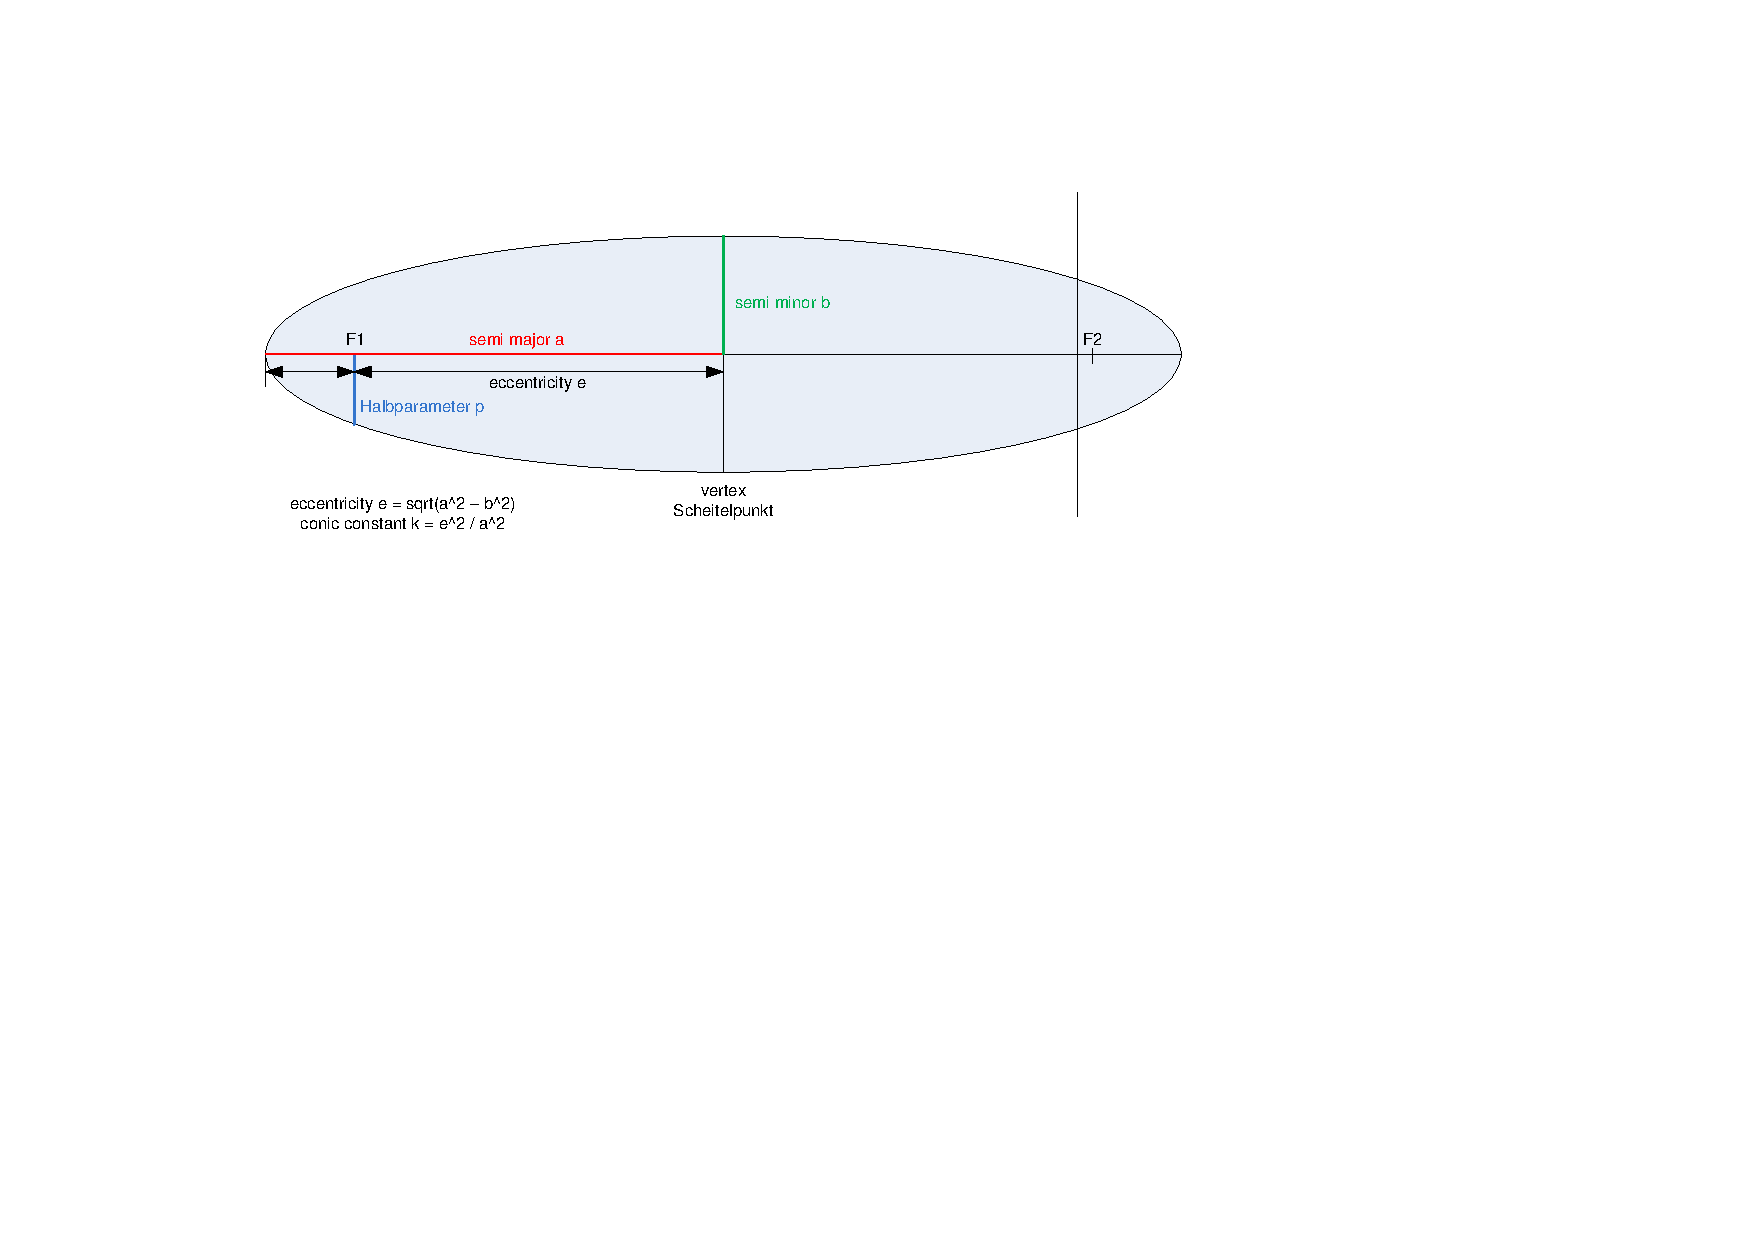
\includegraphics[width=0.8\textwidth]{images/visio/visio.pdf}
	\caption{Ideenskizze}
	\label{fig.Skizze}
\end{figure}

So kann die Abbildung~\ref{fig.Skizze} referenziert werden. Bei der PDF Erstellung ist darauf zu achten, dass LaTeX nur Versionen bis 1.4 voll unterstützt. 



\subsection{Graphiken in LaTeX zuschneiden}\label{zuschneiden}
Mit dem Befehl Clip kann eine Graphik auch in LaTeX zugeschnitten werden:

\begin{figure}[H]
	\centering
		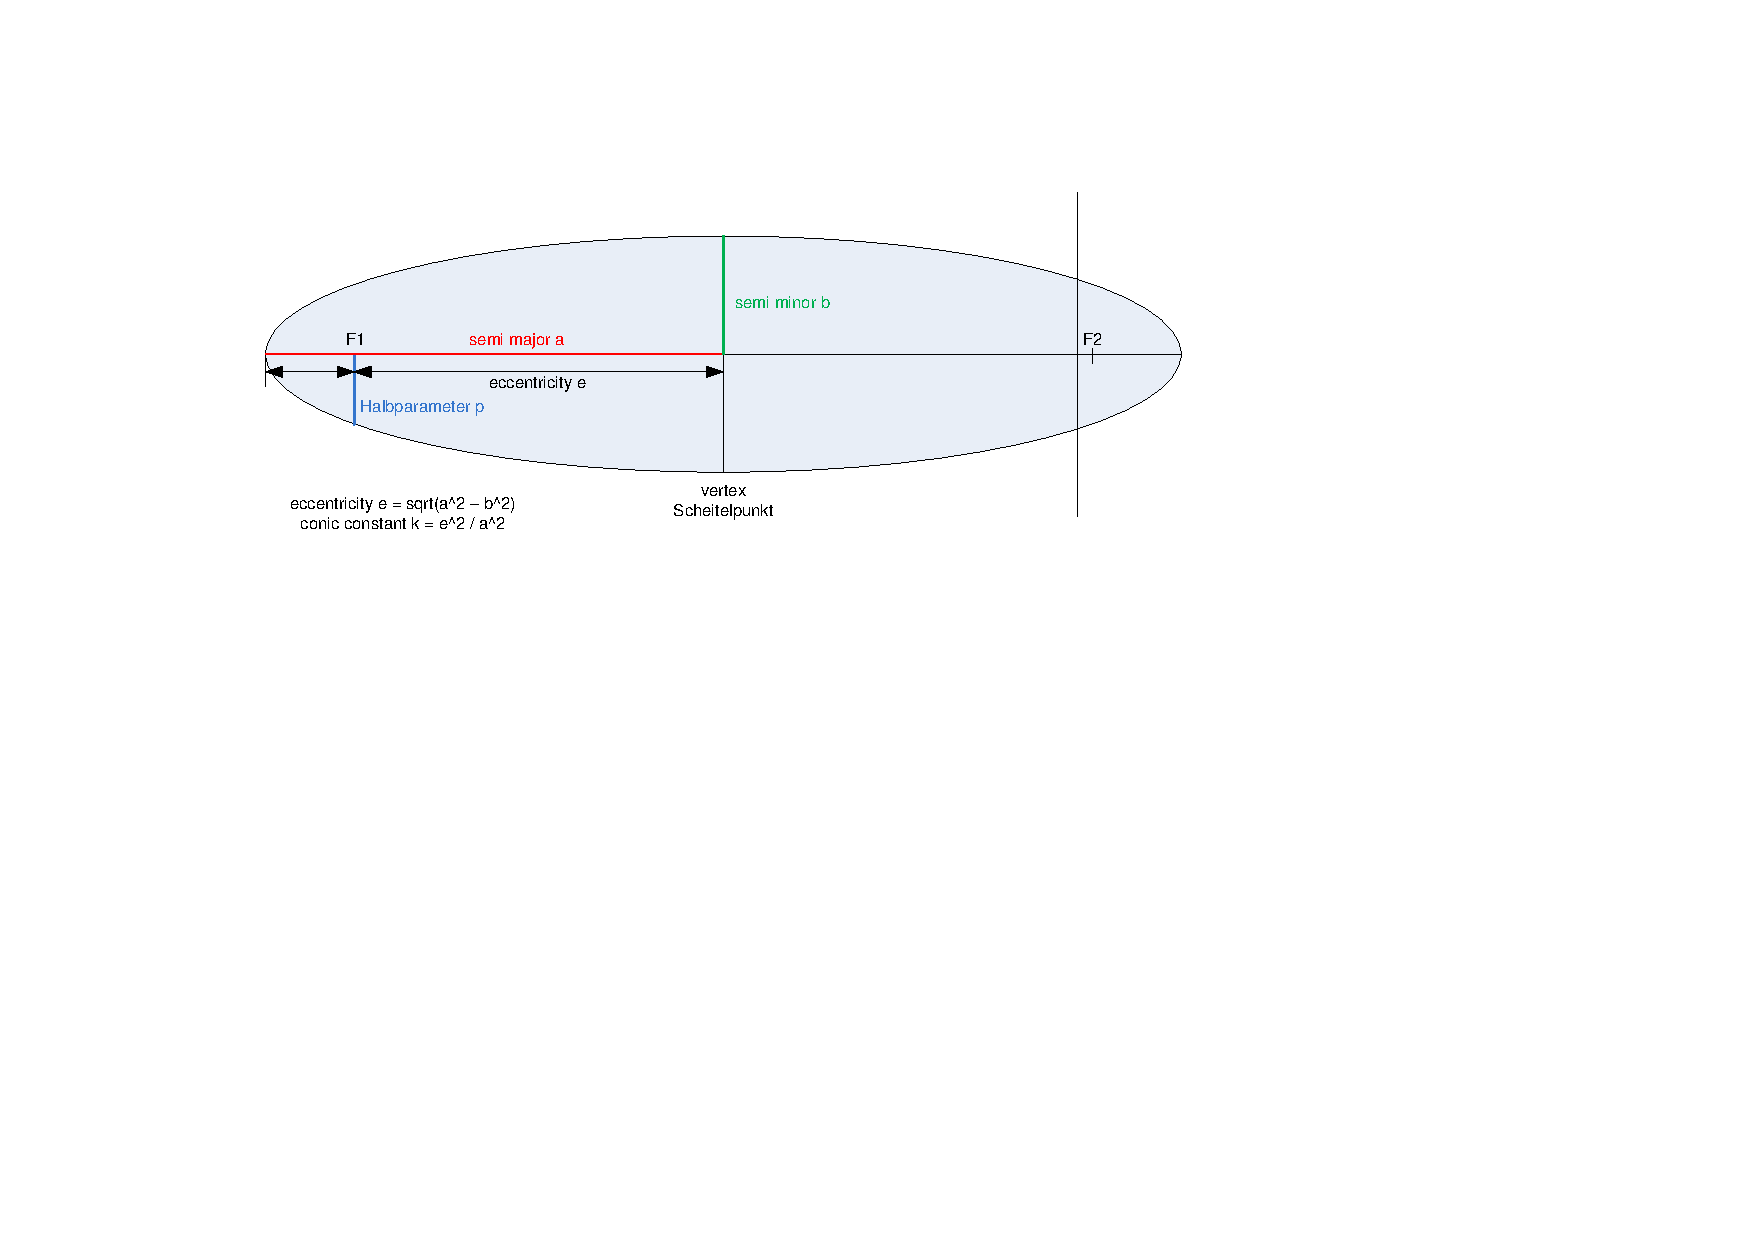
\includegraphics[width=0.9\textwidth, clip=true, trim = 80 10 0 10]{images/visio/visio.pdf}  % trim lm bm rm tm (left, bottom, right, top)
	\caption{clip=true, trim = 60 10 0 10}
	\label{fig.SkizzeZugeschnitten}
\end{figure}



\subsection{Mehrere Bilder nebeneinander}\label{nebeneinander}
Dank Minipages können mehrere Bilder auch nebeneinander sein:

%Zwei Bilder nebeneinander http://latex.mschroeder.net/
\begin{figure}[H]
  \centering
  \begin{minipage}[b]{0.45\textwidth}
    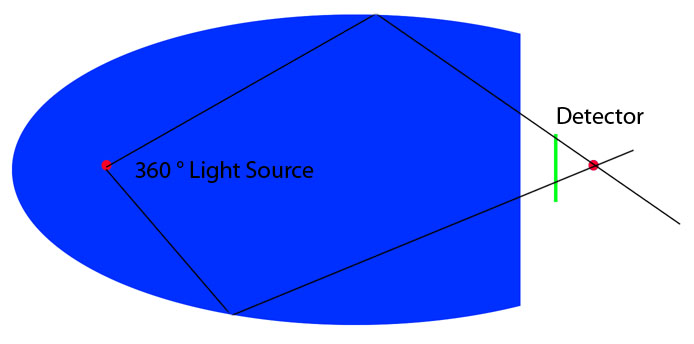
\includegraphics[scale=0.15]{images/photoshop/Skizze.jpg}
    \caption{Visir10b Detector}
    \label{Visir10bDetector} 
  \end{minipage} % Hier darf keine Leerzeile zwischen den beiden Minipages liegen!
  \begin{minipage}[b]{0.45\textwidth}
    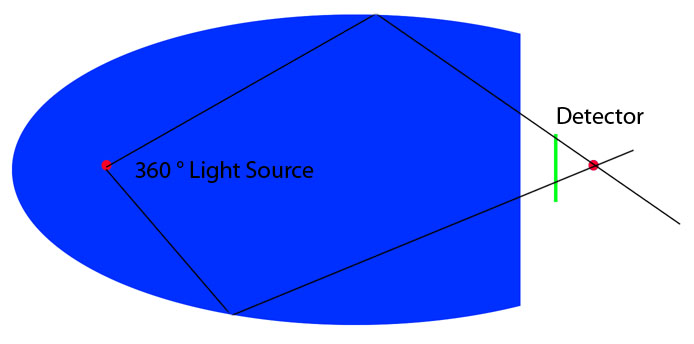
\includegraphics[scale=0.15]{images/photoshop/Skizze.jpg} 
    \caption{Visir10b Model}
    \label{Visir10bModel} 
  \end{minipage}
  \caption{Visir 10 mit optimiertem Reflektor}
  \label{fig.Visir10b}
\end{figure}


Literaturverweis: \citep[S.21]{analog_devices_dac}

\section{Tabellen aufbauen}\label{tabelle}
Kleine Tabelle:

\begin{table}[ht] \centering
	\begin{tabular}{|p{3cm}|p{.5cm}|p{.5cm}|p{.5cm}|p{.5cm}|p{.5cm}|p{.5cm}|p{.5cm}|p{.5cm}|p{.5cm}|p{.5cm}|} \hline
		\rowcolor{gray} Modul & M01 & M02 & M03 & M04 & M05 & M06 & M07 & M08 & M09 & M10 \\
		\hline
		FPGA\_DATEN & & & & & X & X & & X & X & \\
		\hline
		IRQ & X & X & X & & X & & & & X & X \\
		\hline
		Nachbar Core & & & & X & & X & & X & & \\
		\hline
	\end{tabular}
	\caption{Port Schwierigkeiten der Funkmodule}
	\label{tab:portprobleme}
 \end{table}	

Die nachfolgende longtable kann sich über mehrere Seiten erstrecken.

\begin{longtable}{|p{1.1cm}|p{4cm}|p{4cm}|p{4cm}|} 
					\hline
					\rowcolor{gray} Typ & Variante A & Variante B & Variante C
					\\ \hline
					& \textbf{Vorteile:} 
							\begin{itemize}
								\item[+] hohe Spannungen
							\end{itemize}							
							\textbf{Nachteile:}
							\begin{itemize}
								\item[-] Grosse Abmessung
							\end{itemize}
					& 	\textbf{Vorteile:} 
							\begin{itemize}
								\item[+] einfache Montage
							\end{itemize}							
							\textbf{Nachteile:}
							\begin{itemize}
								\item[-] max. 2A Eingangsstrom
							\end{itemize}
					&	\textbf{Vorteile:} 
							\begin{itemize}
								\item[+] hoher Strom
							\end{itemize}							
							\textbf{Nachteile:}
							\begin{itemize}
								\item[-] max. 12 V Eingangsspannung
							\end{itemize}\\ \hline
						Zeit & 2 h & 5 h & 3 h \\ \hline
						Preis	& 520 CHF/Stück & 800 CHF/Stück &	360 CHF/Stück\\ \hline
				\caption{Morphologischer Kasten für die Speisung}
				\label{tab:morphkasten}
			\end{longtable}	

Diese Art von Tabelle erstreckt sich immer auf der ganzen Seitenlänge:

\begin{tabularx}{\textwidth}{XXl}
  Salat & Schnecke & Igel\\
  Montag & Hier ist ein langes Wort & Dienstag
\end{tabularx}



\section{Code Listings aufbauen}\label{listing}

\begin{lstlisting}[
    language=C++,
    caption={Test Kommandozeilen Ausgabe},
    label={list.Testoutput}
]
/********************************************************/
/* Name        : M07Setup                               */
/* Description : EM9201 init for adress and pck         */
/* Input       : targetadr (DevAdr_M00 - DevAdr_M39)    */
/*               drate (Drate_M00 - Drate_M39)          */
/* Ouput       : -0x01 -> Setup OK                      */
/*               -0x5E -> Setup Error Channel write     */
/*               -0x6E -> Setup Error power write       */
/*               -0x7E -> Error in Device Address       */
/*               -0x8E -> Error in Peer Address         */
/********************************************************/
\end{lstlisting}

Formula $e = \sqrt{a{^2} - b^{2}}$


Diese Textstelle ist sehr interessant.\label{interessant}\\
Hier wird auf die Textstelle~\ref{interessant} verwiesen, die sich auf der Seite~\pageref{interessant} befindet.


% nogo:
% \ref{src:miktex} (\nameref{src:miktex})



\section{Citation nach IEEE}\label{citation}

Das ist ein \cite{robotvision} Verweis aufs Literaturverzeichnis. Ein anderes Beispiel ist das hier \cite{randompatterns}.





Das ist eine Aufzählung:
\begin{itemize} %
	\item Erste Zeile
	\item Zweite Zeile
	\item Dritte Zeile
\end{itemize}


\begin{enumerate}
\item erstens
\item zweitens
\end{enumerate}

%https://parma.zhaw.ch/svn/zhw_latex/
%gmanstyle nötig unter start od begin einbinden


Das ist eine verschachtelte Aufzählung:
\begin{description}
		\item [Register Performance] Alle Signale die das FPGA nicht verlassen, also von FF zu FF weitergeleitet werden. Daraus ergibt sich die maximale Taktfrequenz F\textsubscript{MAX}.

		\item [Externes Timing] FPGA Ein- und Ausgänge
		\begin{itemize}
			\item Ausgänge = Von FF's durch Logik zu Ausgängen (t\textsubscript{CO})
			\item Eingänge = Von Eingängen durch Logik zu FF's (t\textsubscript{SU}, t\textsubscript{H})
			\item Durchgänge = kombinatorische Pfade durch das FPGA (t\textsubscript{PD})
		\end{itemize}
\end{description}
 % Für das Schlussdokument auskommentieren

%%%%%%%%%%%%%%%%%%%%%%%%%%%%%%%%%%%%%%%%%%%%%%%%%%%%%%%%%%%%%%%%%
%
% Project     : Turnverein App
% Title       : 
% File        : uebersicht.tex Rev. 00
% Date        : 07.07.14
% Author      : Raffael Santschi
%
%%%%%%%%%%%%%%%%%%%%%%%%%%%%%%%%%%%%%%%%%%%%%%%%%%%%%%%%%%%%%%%%%

\chapter{Projektübersicht}\label{chap.projektuebersicht}

Die Übersicht dient dem Zweck, eine generelle Übersicht über das Dokument zu verschaffen. Sie beinhaltet die Ausganglage, das Ziel dieser Arbeit, die Aufgabenstellung, die erwarteten Resultate und die Nicht-Ziele. Zusätzlich wird der Aufbau dieses Dokumentes erklärt.

\section{Ausgangslage}\label{ausganglage}
Der Turnverein Grafstal wünscht sich auf sein 125-jähriges Jubiläum ein Mobile App. Der Verein hat bereits eine interaktive Webseite, welche in PHP geschrieben ist. Die Nutzung der Webseite wird immer grösser und bis jetzt werden ca. 800 Mitglieder damit verwaltet. In der letzten Zeit hat es sich eingebürgert, dass die Mitglieder sich per Whatsapp organisieren, wer ins Training fährt und wie viel Platz er noch im Auto hat. Dies und das Abrufen der wichtigsten Informationen sollen über das App möglich sein.

\section{Ziele der Arbeit}\label{ziele}
Das Ziel ist eine Mobile App zu entwickeln, welche die wichtigsten Grundfunktionen (neueste Berichte anzeigen, Trainings-, Anlass-, Matchinformationen und die dazugehörigen An- und Abmeldefunktionen für die jeweiligen Events) abdeckt. Die wichtigste Funktion neben den Informationen ist die Fahrgemeinschaftsverwaltung. Durch diese Verwaltung soll der Whatsapp Chat entlastet und eine saubere Abwicklung gewährleistet werden. Der Verein erhofft sich vom App im Weiteren eine höhere Anmeldungsquote, da das Anmelden durch wenige Klicks ermöglichst werden sollte. Zusätzlich kann bei der App die Push-Funktion genutzt werden, um Mitglieder auf Wichtiges aufmerksam zu machen. Für die Zukunft hat ein App weitere Vorteile, da auf GPS-Daten zugegriffen  und offline Caching eingebaut  werden kann, diese beiden Eigenschaften sind jedoch nicht Teil dieser Arbeit.

\section{Aufgabenstellung}\label{aufgabenstellung}
Folgende Punkte werden in der Semesterarbeit behandelt:
\begin{itemize}
\item Analysieren des Ist-Zustands
\item Anforderungen an die Fahrgemeinschaftsverwaltung
\item Entwicklung einer Mobile App mit Login
\item Entwicklung einer Fahrgemeinschaftsverwaltung mit geeignetem Locking-Verfahren
\item Abnahme der Mobile App durch den Vorstand
\end{itemize}

\section{Erwartete Resultate}\label{erwartete_resultate}
Folgende Punkte werden als Resultate der Semesterarbeit erwartet:
\begin{itemize}
\item Dokumentation des Ist-Zustandes
\item Anforderungskatalog
\item Beschreibung der Architektur und Locking-Verfahren bei der Fahrgemeinschaftsverwaltung
\item Implementation der gewünschten Funktionen in einem Mobile App
\item Live Schaltung des erweiterten Backends und Bereitstellung der App für den Download
\end{itemize}

\section{Nicht-Ziele}\label{nicht_ziele}
Folgende Punkte wurden mit dem Auftraggeber als Nicht-Ziele definiert und sind somit nicht Teil dieses Projekts:
\begin{itemize}
\item Dieses Projekt erweitert die Funktionalität der Webseite nicht
\item Es müssen keine Tests für die alten Funktionen geschrieben werden, es sei denn, sie werden im Rahmen dieses Projekts umgeschrieben
\item Die Vermarktung des Apps ist Sache des Auftraggebers
\item Lokales Speichern der Daten im App ist in diesem Prototyp noch nicht notwendig
\end{itemize}

\section{Dokumentstruktur}\label{nicht_ziele}
Dieses Dokument spiegelt die geleistete Arbeit wieder und ist in einzelne Kapitel unterteilt.
\begin{itemize}
\item Projektplanung: Schritte für die Erstellung des Projektplanes und Risikoanalyse
\item Anforderungsdokument: System- und Kontextabgrenzung, Stakeholderliste, getroffene Annahmen und der Anforderungskatalog mit Use Cases, Mockups und Anforderungen
\item Architektur: Übersicht über das ganze System, Nutzwertanalyse der verschiedenen Lösungsvarianten sowie Architektur-Beschreibung von Backend und App
\item Umsetzung: Beschreibung der Entwicklungsumgebung, Umsetzung von App und Backend
\item Tests: Erläuterung der Test-Methoden sowie des Abnahme-Protokolls
\end{itemize}

Im Kapitel \ref{chap.verzeichnisse} sind alle Verzeichnisse zu finden, darunter auch ein Glossar, in welchem unbekannte Begriff erklärt werden. Falls es zu einem gewissen Begriff eine gängige Abkürzung gibt, wird diese beim ersten Auftauchen des Wortes in Klammern geschrieben und danach verwendet, im Glossar finden sich dann beide Einträge.

%%%%%%%%%%%%%%%%%%%%%%%%%%%%%%%%%%%%%%%%%%%%%%%%%%%%%%%%%%%%%%%%%
%
% Project     : Turnverein App
% Title       : 
% File        : projektplanung.tex Rev. 00
% Date        : 07.07.14
% Author      : Raffael Santschi
%
%%%%%%%%%%%%%%%%%%%%%%%%%%%%%%%%%%%%%%%%%%%%%%%%%%%%%%%%%%%%%%%%%

\chapter{Projektplanung}\label{chap.projektplanung}
Dieses Kapitel handelt von der Projektplanung und den verschiedenen Arbeitspakete in diesem Projekt.

\section{Meilensteine}\label{meilensteine}
Folgende Meilensteine wurden für dieses Projekt festgelegt:

\begin{table}[ht]
\centering
  \begin{tabular}{ l | r }
	\hline
	\rowcolor{gray}
	Projektstart:					&	01.04.2014	\\ \hline
	Anforderungsdokument Entwurf		&	07.05.2014	\\ \hline
	Anforderungsdokument fertig		&	12.07.2014	\\ \hline
	Refactoring abgeschlossen		&	04.08.2014	\\ \hline
	App und Backend implementiert		& 	30.08.2014	\\ \hline
	Test-Phase abgeschlossen			&	02.09.2014	\\ \hline
	App zur Freigaben eingesendet		&	02.09.2014	\\ \hline
	Dokumentation fertig			&	20.09.2014	\\ \hline
	Dokumentation korrigiert			&	27.09.2014	\\ \hline
  \end{tabular}
   \caption{Meilensteine}\label{table:milestones}
\end{table}

\section{Arbeitspakete}\label{arbeitspakete}
Das Projekt beinhaltet sechs Arbeitspakete:
\begin{itemize}
\item Planung
\item Requirement Engineering
\item Refactoring Backend
\item Entwicklung Mobile App
\item Testing
\item Dokumentation
\end{itemize}

\subsection{Planung}\label{planung}
In der Planungsphase wird geschaut, was in dem Projekt erreicht werden muss und wie diese Tätigkeiten auf die vorhandene Zeit aufgeteilt wird. Es wird auch das erste Mal mit den Stakeholdern geredet und erste Abmachungen getroffen.

\subsection{Requirement Engineering}\label{rqe}
Bei der Erstellung eines neuen Systems ist es immer wichtig, dass man alle Anforderungen kennt. Um die Anforderungen zu erfassen werden die Mitglieder und der Vorstand befragt, was sie sich von dem App wünschen. Die Mitglieder sind nur zum Teil Techniker, somit werden auch Anforderungen eintreffen, welche sehr schwierig um zu setzten sind und andere Anforderungen werden nicht aufgelistet, sondern einfach vorausgesetzt, sogennante Basisfaktoren. Der Anforderungskatalog wird mit den Mitgliedern, welche sich eingebracht haben, angeschaut und am Schluss findet ein Review statt. (siehe dazu auch \cite{req_eng_book})

\subsection{Refactoring Backend}\label{ref_backend}
Als erste Entwicklungstätigkeit muss das Backend umgebaut werden, damit die Implementation für das Mobile App leichter fällt. Dazu wird der Ist-Stand aufgenommen und geschaut, welche Klassen umstrukturiert werden müssen, damit es danach leichter fällt. Danach wird entschieden, welches Pattern man beim Umbau der Klassen verfolgen möchte. Das Umbauen ist mit viel Arbeit und Testen verbunden.

\subsection{Entwicklung Mobile App}\label{eng_app}
In diesem Arbeitspaket werden die Anforderungen umgesetzt. Das App wird entworfen und mit Inhalt gefüllt. Die ersten Tests werden durchgeführt und Unstimmigkeiten in den Anforderungen werden mit den Stakeholdern angeschaut.

\subsection{Tests}\label{tests}
Es gibt zwei Testsphasen, die eine ist dann, wenn das neue Backend online ist und die User, wie gewohnt, arbeiten können sollten. Die andere besteht darin, dass  das App für Android zum Download bereit gestellt wird, nachdem die ersten Tests erfolgreich waren.  Das Feedback wird bei beiden Phasen eingearbeitet und möglichst schnell aktualisiert.

\subsection{Dokumentation}\label{dokumentation}
Die Dokumentation wird das ganze Projekt hindurch aktuell gehalten. Für das Erfassen dieses Dokuments wird \LaTeX\ und das \LaTeX-Template der ZHAW verwendet.


\newpage
\section{Projektstrukturplan}\label{projektstrukturplan}
Anhand der Arbeitspakten wurde ein Projektstrukturplan (siehe Abbildung \ref{fig:psp}) erstellt, welcher die Arbeitspakete in Teilaufgaben unterteilt. Diese Methode ist aus \cite{proj_mgmt_book} bekannt.
\begin{figure}[h]
\centering
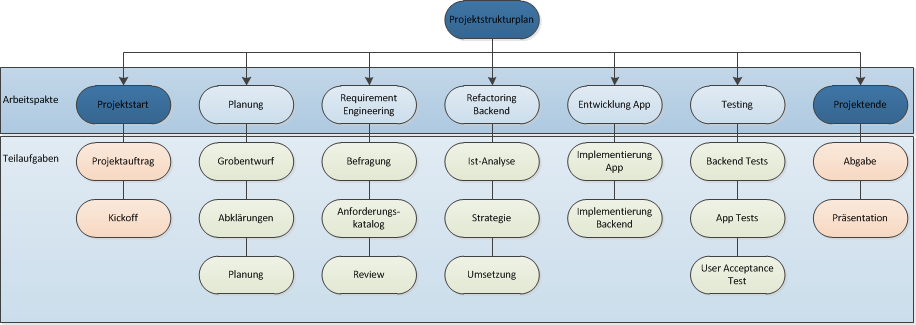
\includegraphics[scale=0.7]{images/visio/PSP.png}
\caption{Projektstrukturplan}
\label{fig:psp}
\end{figure}



\section{Zeitplan}\label{zeitplan}
Der Zeitplan gibt eine grobe Übersicht, wann an dem Projekt gearbeitet wird und wann die verschiedenen Tätigkeiten fertig werden. Die Angaben sind nur Richtwerte, da neben diesem Projekt noch einer Arbeit nachgegangen wird, verschiedenen Tätigkeiten im Verein ausgeführt werden und zusätzliche andere Arbeiten und Prüfungen Zeit benötigen.

\subsection{Geplante Abwesenheiten}
\begin{table}[ht]
\centering
  \begin{tabular}{ l | r }
	\hline
	\rowcolor{gray}
	Abwesenheit							&	Start - Ende	\\ \hline
	Seminararbeit Abgaben					&	01.06.2014 - 22.06.2014	\\ \hline
	Modulprüfungen und Vorträge Seminararbeit		&	23.06.2014 - 02.07.2014	\\ \hline
	Ferien								&	12.07.2014 - 03.08.2014	\\ \hline
  \end{tabular}
   \caption{Geplante Abwesenheiten}\label{table:holidays}
\end{table}

\begin{landscape}
\thispagestyle{empty}
\subsection{Projektplan}\label{projektplan}
Der Zeitplan basierend auf dem Projektstrukturplan (siehe \ref{projektstrukturplan})  und den geplanten Abwesenheiten sieht wie folgt aus:
\begin{figure}[h]
\centering
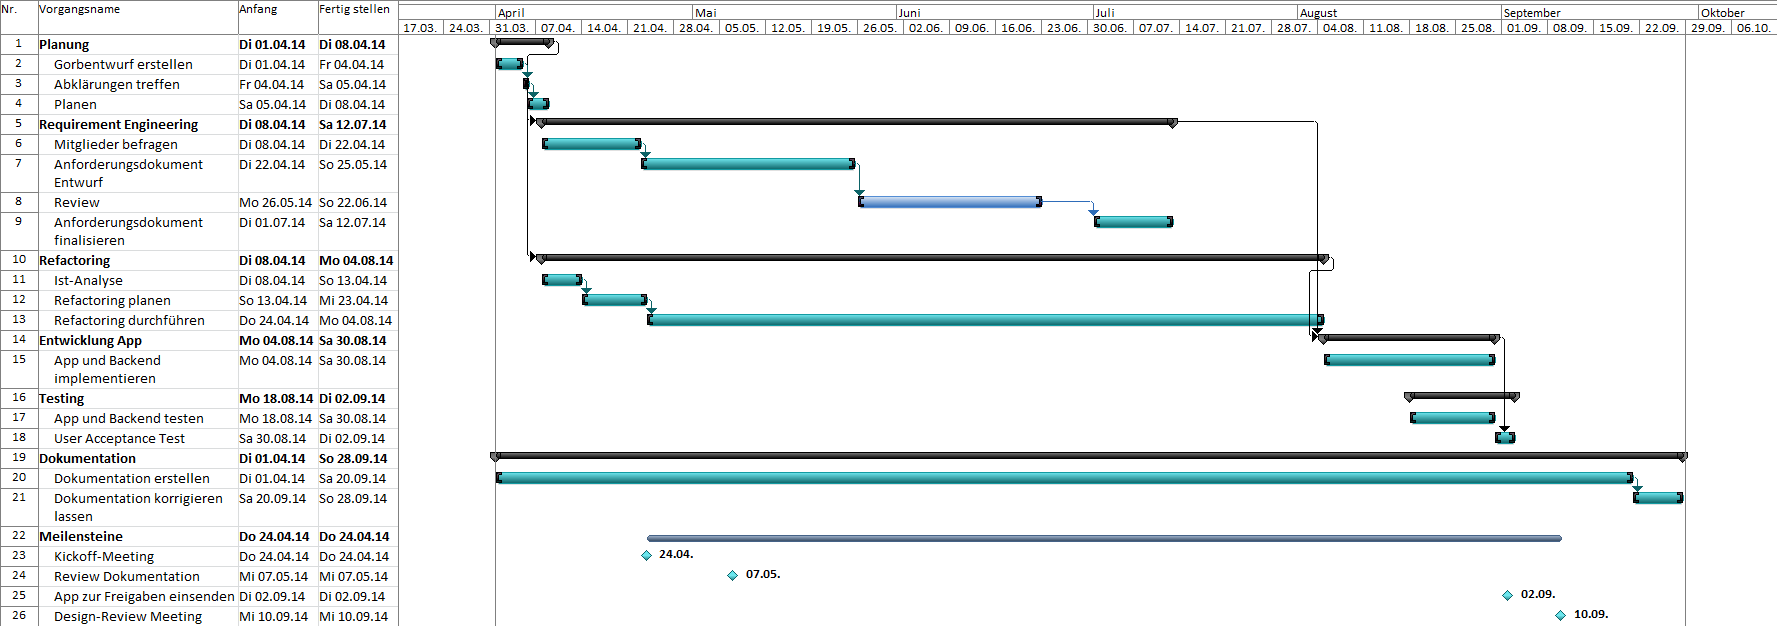
\includegraphics[scale=0.5]{images/project/projectplan.png}
\caption{Projektplan}
\label{fig:psp}
\end{figure}

\end{landscape}

\subsection{Zeitschätzung auf Arbeitspaketebene}
\begin{table}[ht]
\centering
  \begin{tabular}{ l | c | c }
	\hline
	\rowcolor{gray}
	Arbeitspaket							&	Schätzung (h)	& Tatsächlich (h)	\\ \hline
	Planung							&	10			& 8	\\ \hline
	Requirement Engineering					&	12			& 15	\\ \hline
	Refactoring Backend					&	20			& 40	\\ \hline
	Entwicklung Mobile App					&	45			& 50	\\ \hline
	Tests								&	8			& 10	\\ \hline
	Dokumentation						&	60			& 70	\\ \hline \hline
	Total								&	155			& 193	\\ \hline
  \end{tabular}
   \caption{Zeitschätzung auf Arbeitspaketebene}\label{table:time_estimation}
\end{table}

\section{Risikoanalyse}\label{risikoanalyse}
Jedes Projekt bringt Risiken mit sich, wenn diese nicht am Anfang analysiert und durch das ganze Projekt überprüft werden, kann es zu grossen Schwierigkeiten kommen. Die angewandten Methoden sind aus \cite{proj_mgmt_book} und aus dem dem Management Fach Projekt und Prozessmanagement bekannt.

\subsection{Risikoermittlung}\label{risikoermittlung}
Die Risikoermittlung ist dafür da, dass man mögliche Risiken aufdeckt und die möglichen Folgen daraus festhält.

\begin{table}[ht]
\centering
  \begin{tabular}{  p{5cm} | p{9cm} }
	\hline
	\rowcolor{gray}
	Risiko							&	Mögliche Folgen	\\ \hline
	Implementationsschwierigkeiten (Nur wenig Erfahrung in der App Entwicklung)
								&	\begin{itemize}
										\item Zeitplan nicht einhaltbar
										\item Einige Anforderungen müssen zurück gestellt werden
										\item Projektarbeit kann nicht durchgeführt werden
									\end{itemize}	\\ \hline
	Ressourcen nicht verfügbar
								&	\begin{itemize}
										\item Zeitplan nicht einhaltbar
										\item Einige Anforderungen müssen zurück gestellt werden
										\item Projektarbeit kann nicht durchgeführt werden
									\end{itemize}	\\ \hline
	Mangelhaftes Endprodukt		
								&	\begin{itemize}
										\item Produkt muss überarbeitet werden, da keine Abnahme durch die Stakeholder erfolgt
									\end{itemize}	\\ \hline	
	Anforderungen nicht vollständig	
								&	\begin{itemize}
										\item Wichtige Funktionen stehen den Benutzern nicht zur Verfügung
									\end{itemize}	\\ \hline			
  \end{tabular}
   \caption{Risikoermittlung}
\end{table}

\subsection{Risikobewertung}
Das Schadensausmass und die Eintrittswahrscheinlichkeit der Risiken sind nach folgendem Schema bewertet worden:

\begin{table}[ht]
\centering
  \begin{tabular}{ l | p{5cm} | p{5cm} }
	\hline
	\rowcolor{gray}
	Wert							&	Eintrittswahrscheindlichkeit	&	Schadensausmass	\\ \hline			
	1							&	sehr unwahrscheinlich		&	vernachlässigbar	\\ \hline
	2							&	unwahrscheinlich			&	spürbar		\\ \hline
	3							&	wenig wahrscheinlich		&	verkraftbar		\\ \hline
	4							&	ziemlich wahrscheinlich		&	gefährlich		\\ \hline
	5							&	sehr wahrscheinlich			&	katastrophal		\\ \hline
  \end{tabular}
   \caption{Risikobewertungsschema}
\end{table}

\FloatBarrier
Die Risiken aus der Risikobewertung (siehe \ref{risikoermittlung}) wurden anhand dieses Schemas bewertet.

\begin{equation*}
Risikofaktor = Eintrittswahrscheindlichkeit * Schadensausmass
\end{equation*}

\begin{table}[ht]
\centering
  \begin{tabular}{ l | p{4cm} | p{3cm} | c }
	\hline
	\rowcolor{gray}
	Risiko							&	Eintrittswahrscheindlichkeit	&	Schadensausmass 	&	Risikofaktor\\ \hline			
	Implementationsschwierigkeiten			&	1					&	4			&	4		\\ \hline
	Ressourcen nicht verfügbar			&	2					&	5			&	\textbf{10}	\\ \hline
	Mangelhaftes Endprodukt				&	2					&	4			&	\textbf{8}	\\ \hline
	Anforderungen nicht vollständig			&	3					&	3			&	\textbf{9}	\\ \hline
  \end{tabular}
   \caption{Risikobewertung}
\end{table}

\subsection{Risikomatrix}
Anhand der Risikobeurteilung konnten die Risiken in eine Risikomatrix eingesetzt werden. Diese Matrix bietet einen guten Überblick über die Risiken und zeigt schnell, welche Risiken beachtet werden müssen.
\begin{figure}[h]
\centering
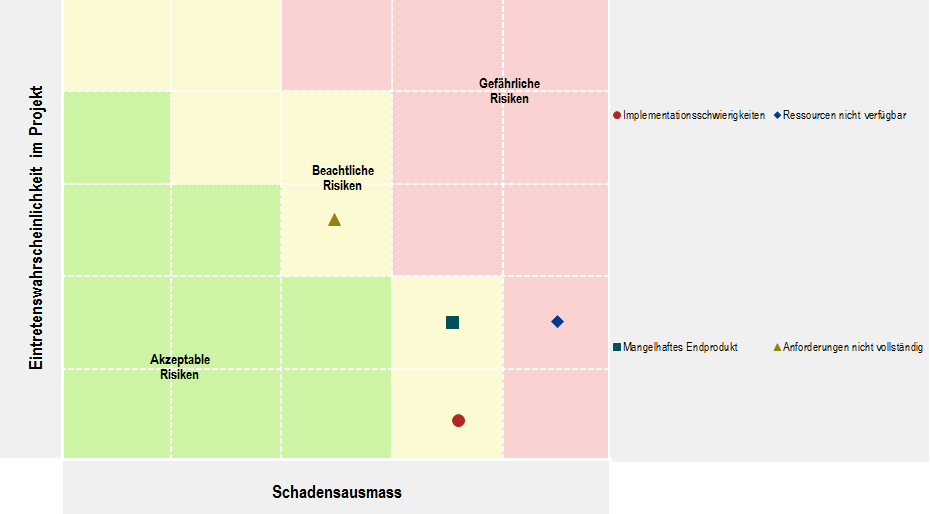
\includegraphics[scale=0.5]{images/excel/risikomatrix.png}
\caption{Risikomatrix}
\label{fig:risikomatrix}
\end{figure}

\subsection{Massnahmen}
Es wurden Massnahmen für die gefundenen Risiken gesucht und festgehalten. Die Massnahmen sind wiederum in vorbeugende Massnahmen und Eventualmassnahmen unterteilt.

\begin{table}[ht]
\centering
  \begin{tabular}{  l | p{4cm} | p{4cm} }
	\hline
	\rowcolor{darkgray}
	Risiko							&	\multicolumn{2}{|c|}{Massnahmen} \\ \hline
	\rowcolor{gray}
								&	Vorbeugende Massnahmen & Eventualmassnahmen	\\ \hline
	Implementationsschwierigkeiten
								&	\begin{itemize}
										\item Im Zeitplan genügen Reserver einrechnen
										\item Kontaktpersonen zum Thema suchen
									\end{itemize}
								&	\begin{itemize}
										\item Betreuer / Schulleitung informieren
										\item Verschiebungsgesuch stellen
									\end{itemize}						\\ \hline
	Ressourcen nicht verfügbar
								&	\begin{itemize}
										\item Fixe Zeiten einplanen
										\item Tätigkeiten priorisieren
									\end{itemize}
								&	\begin{itemize}
										\item Verschiebungsgesuch mit guter Begründung stellen
									\end{itemize}	\\ \hline
	Mangelhaftes Endprodukt		
								&	\begin{itemize}
										\item Anforderungskatalog sauber erstellen
										\item Testphase möglichs früh, damit noch genügen Zeit für die Einarbeitung des Feedbacks ist
									\end{itemize}
								&	\begin{itemize}
										\item Lösung mit dem Kunden suchen
										\item Projekt verlängern
									\end{itemize}	\\ \hline	
	Anforderungen nicht vollständig	
								&	\begin{itemize}
										\item Review des Anforderungskataloges
										\item Testphase möglichs früh, damit noch genügen Zeit für die Einarbeitung des Feedbacks ist
									\end{itemize}
								&	\begin{itemize}
										\item Anforderungen werden aufgenommen und in einen nächsten Release geplant											
									\end{itemize}	\\ \hline			
  \end{tabular}
   \caption{Risikoanalyse - Massnahmen}
\end{table}



%%%%%%%%%%%%%%%%%%%%%%%%%%%%%%%%%%%%%%%%%%%%%%%%%%%%%%%%%%%%%%%%%
%
% Project     : Turnverein App
% Title       : 
% File        : anforderungsdokument.tex Rev. 00
% Date        : 07.07.14
% Author      : Raffael Santschi
%
%%%%%%%%%%%%%%%%%%%%%%%%%%%%%%%%%%%%%%%%%%%%%%%%%%%%%%%%%%%%%%%%%

\chapter{Anforderungsdokument}\label{chap.anforderungsdokument}

Das Anforderungsdokument legt den Grundstein für die Implementation. Es lohnt sich, detaillierte Anforderungen zu erfassen. Einerseits beugt dies vor möglichen Missverständnissen vor, andererseits ist es eine Absicherung, falls am Ende eines Projektes unterschiedliche Ansichten über den Lieferumfang bestünden.

\section{Übersicht}\label{anf_uebersicht}

In diesem Abschnitt werden die System- und Kontextabgrenzung dargelegt, die Systemumgebung beschrieben, die getroffenen Annahmen festgehalten und die verschiedenen \glossarmark{Stakeholder} mit ihren Erwartungen aufgelistet.

\subsection{System- und Kontextabgrenzung}\label{systemabgrenzung}
Der Systemkontext umfasst alle Aspekte, die für die Anforderungen des geplanten Systems relevant sind und nicht im Rahmen der Entwicklung dieses System gestaltet werden können.

Das geplante System hat zwei relevante Schnittstellen zur Aussenwelt, welche die Applikation beeinflussen. Die beiden Push Notification Services \glossarmark{Apple Push Notification Service} (\glossarmark{APNS}) und \glossarmark{Google Cloud Messaging for Android} (\glossarmark{GCM}). Des Weiteren wird das System von den verschiedenen Smartphone Typen, dem Anmeldeprozess, dem Hosting und, nicht zu vergessen, den Mitgliedern beeinflusst.

\cite{req_eng_book} 
\begin{figure}[h]
\centering
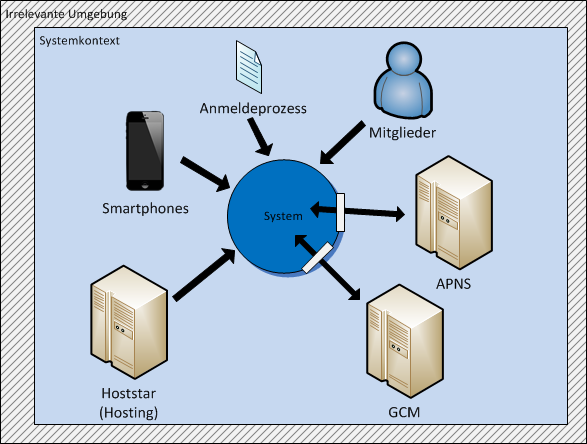
\includegraphics[scale=0.8]{images/visio/systemkontext.png}
\caption{Systemkontext}
\label{fig:systemkontext}
\end{figure}

\FloatBarrier
\subsection{Systemumgebung}\label{systemumgebung}
Die Systemumgebung definiert die Ausgangslage für ein Projekt. Am Anfang des Projekts bestand das System aus einem Webserver, auf dem ein \glossarmark{PHP} Backend und eine interaktive Webseite liefen. Die Daten wurden in einer MySQL Datenbank abgespeichert. 

Die Seite wird rege benutzt, es sind etwa 35 Benutzer pro Tag online. Fast jedes Mitglied besitzt ein Smartphone, wobei die Aufteilung zwischen Android und iOS Geräten etwa ausgeglichen ist. In Abbildung \ref{fig:systemumgebung} ist die Systemumgebung graphisch dargestellt.
\begin{figure}[h]
\centering
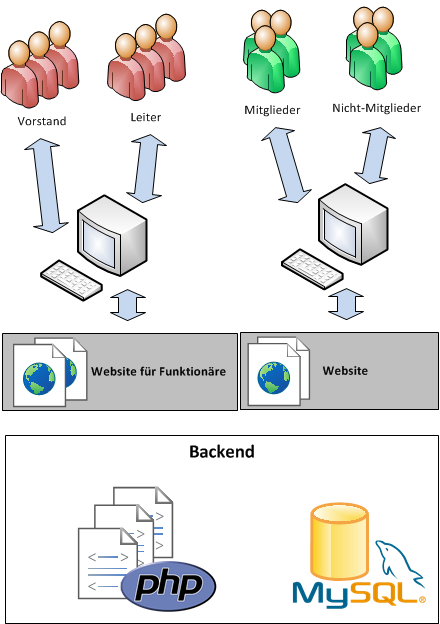
\includegraphics[scale=0.95]{images/visio/systemumgebung.png}
\caption{Systemumgebung}
\label{fig:systemumgebung}
\end{figure}

\FloatBarrier
\subsection{Annahmen}\label{annahmen}
Es mussten keine Annahmen getroffen werden, da durch die enge Zusammenarbeit mit dem Turnverein, alle offenen Punkte in kürzester Zeit geklärt werden konnten.

\newpage
\subsection{Stakeholder}\label{stakeholder}
Die \glossarmark{Stakeholder} Analyse dient dem erfassen aller Nutzergruppen, die auf ein Projekt Einfluss haben. Zudem ermöglicht sie die Erfassung aller Gruppen, die potentiell Anforderungen an das Projekt stellen. In der der Tabelle \ref{table:stakeholder} wurden die \glossarmark{Stakeholder} für dieses Projekt mit der Hilfe des Vorstandes zusammengetragen und ihre Erwartungen, ihre Einstellung und ihr Einfluss gegenüber diesem Projekt festgehalten\footnote{Obwohl in diesem Projekt primär die Bedürfnisse des Turnvereins betrachtet werden, soll die App auch für den Damenturnverein und die Jugensport Kommission nutzbar sein.}. 

\begin{table}[ht]
\centering
  \begin{tabular}{ l | p{5cm} | p{1.5cm} | p{1.5cm} }
	\hline
	\rowcolor{darkgray}
	\textbf{Name}					&	\textbf{Erwartung}	&	\textbf{Einstellung} 	&	\textbf{Einfluss}	\\ \hline
	\rowcolor{gray}
								&				&	-Positiv \mbox{-Neutral} \mbox{-Negativ} 	&	-Hoch \mbox{-Mittel} \mbox{-Niedrig} \\ \hline
	Vorstand						&	Der Vorstand ist der Kunde in diesem Projekt, er hat den Auftrag erteilt. Er erwartet von der App mehr Popularität, vor allem bei den jüngeren Mitgliedern. Zusätzlich erhofft er sich etwas Werbung für den Verein.			
												& 	Positiv		&	Hoch		\\ \hline
	Trainingsverantwortliche				&	Die Trainingsverantwortlichen sehen einen grossen Vorteil darin, dass die Anmeldung für die Trainings vereinfacht werden soll. Sie finden es praktisch, dass sie die Trainingsinformationen schnell abrufen können.			
												& 	Positiv		&	Hoch		\\ \hline
	aktive Mitglieder (U30)				&	Die jüngere Generation der aktiv Mitglieder wartet gespannt auf die App.	Sie wünschen sich eine schnelle Möglichkeit sich anmelden zu können.		
												& 	Positiv		&	Hoch		\\ \hline
	aktive Mitglieder (Ü30)				&	Die ältere Generation der aktiv Mitglieder hat keine grossen Erwartungen an die App, sie würden auch ohne auskommen.		
												& 	Neutral	&	Mittel		\\ \hline
	Passiv- und Ehrenmitglieder			&	Passiv- und Ehrenmitglieder gehören auch eher zu dem älteren Semester und können mit Apps nicht viel anfangen. Sie sind der App gegenüber jedoch nicht negativ eingestellt. Da diese Gruppe einen hohen Einfluss besitzt, ist dies sehr von Vorteil.
												& 	Neutral	&	Hoch		\\ \hline
	Nicht-Mitglieder					&	Die Nicht-Mitglieder erhoffen sich schnelle und gute Informationen über Anlässe und die Vereine selbst.
												& 	Neutral	&	Niedrig	\\ \hline
  \end{tabular}
   \caption{Liste der evaluierten Stakeholder}\label{table:stakeholder}
\end{table}

\newpage
\section{Anforderungen}\label{sec.anfoderungen}
Beim Erfassen der Anforderungen wurden als Erstes die Use-Cases definiert. Diese wurden zusammen mit Vertretern des Turnvereins festgelegt. Die Beschreibung beinhaltet bereits einen klaren Ablauf für die einzelnen Use-Cases. Als nächstes wurden in mehreren Sitzungen die dazugehörigen \glossarmark{Mockups} gestaltet. Bevor die Implementation beginnen konnte, mussten noch die Anforderungen abgeleitet werden. Sie wurden auf der Grundlage einer Mitglieder Befragung und einer kurzen Sitzung mit dem Vorstand evaluiert.

\subsection{Use Cases}\label{use_cases}
Das Use Case Diagramm (siehe Abbildung \ref{fig:use_case}) zeigt zwei Akteure, Mitglieder und Nicht-Mitglieder, sowie sechs Use Cases, welche in diesem Projekt umgesetzt wurden.
\begin{figure}[h]
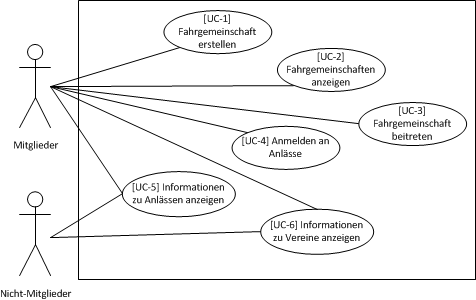
\includegraphics{images/anforderungen/use_cases.png}
\caption{Use-Case Diagramm}
\label{fig:use_case}
\end{figure}

Alle Use Cases wurden anhand der folgenden Vorlage in Tabelle \ref{table:use_case_template} spezifiziert. Diese Schablone basiert auf Angaben von \cite{req_eng_book}. Die Use Cases wurden möglichst genau beschrieben, was danach die Implementation vereinfachte.

\begin{table}[ht]
\centering
  \begin{tabular}{ l | p{10cm} }
	\hline
	\rowcolor{gray}
	\textbf{Bezeichner}		&	Eindeutiger Bezeichner\\ \hline
	\textbf{Name}			&	Eindeutiger Name\\ \hline
	\textbf{Kritikalität}		&	Kritikalität hinsichtlich des Schadensausmasses bei Fehlverhalten: hoch, mittel, leicht\\ \hline
	\textbf{Quelle}			&	\glossarmark{Stakeholder}, Dokument, System\\ \hline
	\textbf{Verantwortlicher}	&	Verantwortlicher \glossarmark{Stakeholder}\\ \hline
	\textbf{Beschreibung}	&	Komprimierte Beschreibung\\ \hline
	\textbf{Auslösendes Ereignis}&	Angabe des Ereignisses, das den Use Case auslöst\\ \hline
	\textbf{Akteure}		&	Auflistung der Akteure, die mit dem Use Case in Beziehung stehen\\ \hline
	\textbf{Vorbedingung}	&	Eine Liste notwendiger Voraussetzungen, die erfüllt sein müssen, bevor die Ausführung des Use Case beginnen kann\\ \hline
	\textbf{Nachbedingung}	&	Eine Liste von Zuständen, in denen sich das System unmittelbar nach der Ausführung des Hauptszenarios befindet.\\ \hline
	\textbf{Ergebnis}		&	Beschreibung der Ausgaben, die während der Ausführung des Use Case erzeugt werden\\ \hline
	\textbf{Hauptszenario}	&	Beschreibung des Hauptszenarios eines Use Case\\ \hline
	\textbf{Alternativszenarien}	&	Beschreibung von Alternativszenarien des Use Case oder lediglich Angabe der auslösenden Ereignisse. 
					Hier gelten oftmals andere Nachbedingungen.\\ \hline
	\textbf{Ausnahmeszenarien}&	Beschreibung von Ausnahmeszenarien des Use Case oder lediglich Angabe der auslösenden Ereignisse. 
					Hier gelten oftmals andere Nachbedingungen.\\ \hline
	\textbf{Mockups}	 	&	Querbezüge zu \glossarmark{Mockups}
  \end{tabular}
   \caption{Vorlage für Use Case Spezifikation}\label{table:use_case_template}
\end{table}

\begin{table}[ht]
\centering
  \begin{tabular}{ l | p{10cm} }
	\hline
	\rowcolor{gray}
	\textbf{Bezeichner}		&	\textbf{UC-1}\\ \hline
	\textbf{Name}			&	Fahrgemeinschaft erstellen\\ \hline
	\textbf{Kritikalität}		&	hoch\\ \hline
	\textbf{Quelle}			&	\glossarmark{Stakeholder}\\ \hline
	\textbf{Verantwortlicher}	&	Marco Mathe (Vorstand)\\ \hline
	\textbf{Beschreibung}	&	Eine der Hauptaufgaben dieser App soll die Fahrgemeinschaftsverwaltung sein. Jedes Mitglied soll eine Fahrgemeinschaft erstellen können.\\ \hline
	\textbf{Auslösendes Ereignis}&	Mitglied möchte eine Fahrgemeinschaft erstellen\\ \hline
	\textbf{Akteure}		&	TV-Mitglied\\ \hline
	\textbf{Vorbedingung}	&	Das Mitglied ist angemeldet und es existiert eine Veranstaltung\\ \hline
	\textbf{Nachbedingung}	&	Das Mitglied hat eine Fahrgemeinschaft erstellt\\ \hline
	\textbf{Ergebnis}		&	Erstellung einer neuen Fahrgemeinschaft\\ \hline
	\textbf{Hauptszenario}	&	\begin{enumerate}
					\item Das Mitglied öffnet den Menü-Knopf
					\item Das System zeigt das Menü an
					\item Das Mitglied klickt auf eine der drei Veranstaltungstypen
					\item Das System fragt eine Liste der Veranstaltungen beim Backend ab
					\item Das System zeigt eine Liste der Veranstaltungen an
					\item Das Mitglied sucht die Veranstaltung und klickt darauf
					\item Das Mitglied klickt auf 'Fahrgemeinschaften'
					\item Das Mitglied klickt auf 'Neue Fahrgemeinschaft'
					\item Das System zeigt ein Formular mit Daten zur Fahrgemeinschaft an
					\item Das Mitglied füllt die Felder aus und sendet das Formular ab
					\item Das System schickt die Daten an das Backend
					\item Das System zeigt 'Fahrgemeinschaft erfolgreich erstellt' an
					\end{enumerate}
					\\ \hline
	\textbf{Alternativszenarien}	&	\begin{enumerate}
					\item[7a] Das System weist das Mitglied auf fehlende Felder hin
					\end{enumerate}
					\\ \hline
	\textbf{Ausnahmeszenarien}&	\begin{enumerate}
					\item[7a] Das System zeigt 'keine Internetverbindung vorhanden' an
					\end{enumerate}
					\\ \hline
	\textbf{Mockups}	 	&	-
  \end{tabular}
   \caption{Use Case UC-1: Fahrgemeinschaft erstellen}\label{table:use_case_1}
\end{table}

\begin{table}[ht]
\centering
  \begin{tabular}{ l | p{10cm} }
	\hline
	\rowcolor{gray}
	\textbf{Bezeichner}		&	\textbf{UC-2}\\ \hline
	\textbf{Name}			&	Fahrgemeinschaften anzeigen\\ \hline
	\textbf{Kritikalität}		&	hoch\\ \hline
	\textbf{Quelle}			&	\glossarmark{Stakeholder}\\ \hline
	\textbf{Verantwortlicher}	&	Marco Mathe (Vorstand)\\ \hline
	\textbf{Beschreibung}	&	Eine der Hauptaufgaben dieser App soll die Fahrgemeinschaftsverwaltung sein. Die Mitglieder sollen sich eine Liste aller Fahrgemeinschaften anzeigen lassen können, um dann zu entscheiden, welcher sie sich anschliessen möchten.\\ \hline
	\textbf{Auslösendes Ereignis}&	Mitglied möchte Fahrgemeinschaften anschauen\\ \hline
	\textbf{Akteure}		&	TV-Mitglied\\ \hline
	\textbf{Vorbedingung}	&	Das Mitglied ist angemeldet und Fahrgemeinschaften sind vorhanden\\ \hline
	\textbf{Nachbedingung}	&	Das Mitglied hat eine Liste von Fahrgemeinschaften erhalten\\ \hline
	\textbf{Ergebnis}		&	Liste von Fahrgemeinschaften\\ \hline
	\textbf{Hauptszenario}	&	\begin{enumerate}
					\item Das Mitglied öffnet den Menü-Knopf
					\item Das System zeigt das Menü an
					\item Das Mitglied klickt auf eine der drei Veranstaltungstypen
					\item Das System fragt eine Liste der Veranstaltungen beim Backend ab
					\item Das System zeigt eine Liste der Veranstaltungen an
					\item Das Mitglied sucht die Veranstaltung und klickt darauf
					\item Das Mitglied klickt auf 'Fahrgemeinschaften'
					\item Das System fragt eine Liste der Fahrgemeinschaften beim Backend ab
					\item Das System zeigt eine Liste der Fahrgemeinschaften an
					\end{enumerate}
					\\ \hline
	\textbf{Alternativszenarien}	&	\begin{enumerate}
					\item[5a] Das System zeigt 'keine aktuellen Fahrgemeinschaften' an
					\end{enumerate}
					\\ \hline
	\textbf{Ausnahmeszenarien}&	\begin{enumerate}
					\item[4a] Das System zeigt 'keine Internetverbindung vorhanden' an
					\end{enumerate}
					\\ \hline
	\textbf{Mockups}	 	&	\ref{fig:mockup_navigation}, \ref{fig:mockup_carpools}, \ref{fig:mockup_carpool_detail},
					\ref{fig:mockup_add_carpool}
  \end{tabular}
   \caption{Use Case UC-2: Fahrgemeinschaften anzeigen}\label{table:use_case_2}
\end{table}


\begin{table}[ht]
\centering
  \begin{tabular}{ l | p{10cm} }
	\hline
	\rowcolor{gray}
	\textbf{Bezeichner}		&	\textbf{UC-3}\\ \hline
	\textbf{Name}			&	Fahrgemeinschaft beitreten\\ \hline
	\textbf{Kritikalität}		&	hoch\\ \hline
	\textbf{Quelle}			&	\glossarmark{Stakeholder}\\ \hline
	\textbf{Verantwortlicher}	&	Marco Mathe (Vorstand)\\ \hline
	\textbf{Beschreibung}	&	Eine der Hauptaufgaben dieser App soll die Fahrgemeinschaftsverwaltung sein. Beim Beitreten einer Fahrgemeinschaft geht es darum, dass das Mitglied Interesse an der Fahrgemeinschaft hat und dieser gern beitreten möchte.\\ \hline
	\textbf{Auslösendes Ereignis}&	Mitglied möchte einer Fahrgemeinschaft beitreten\\ \hline
	\textbf{Akteure}		&	TV-Mitglied\\ \hline
	\textbf{Vorbedingung}	&	Das Mitglied ist angemeldet und Fahrgemeinschaften sind vorhanden\\ \hline
	\textbf{Nachbedingung}	&	Das Mitglied ist einer Fahrgemeinschaft beigetreten\\ \hline
	\textbf{Ergebnis}		&	Neuer Eintrag in der Gemeinschaft und Kapazitätenminderung\\ \hline
	\textbf{Hauptszenario}	&	\begin{enumerate}
					\item Das Mitglied öffnet den Menü-Knopf
					\item Das System zeigt das Menü an
					\item Das Mitglied klickt auf eine der drei Veranstaltungstypen
					\item Das System fragt eine Liste der Veranstaltungen beim Backend ab
					\item Das System zeigt eine Liste der Veranstaltungen an
					\item Das Mitglied sucht die Veranstaltung und klickt darauf
					\item Das Mitglied klickt auf 'Fahrgemeinschaften'
					\item Das System zeigt eine Liste aller Fahrgemeinschaften an
					\item Das Mitglied wählt eine aus und klickt auf 'Beitreten'
					\item Das System zeigt 'Erfolgreich beigetreten' an
					\end{enumerate}
					\\ \hline
	\textbf{Alternativszenarien}	&	\begin{enumerate}
					\item[3a] Das System zeigt 'Kein Platz mehr' an
					\item[4] Der User wählt eine andere Fahrgemeinschaft aus und versucht es erneut
					\end{enumerate}
					\\ \hline
	\textbf{Ausnahmeszenarien}&	\begin{enumerate}
					\item[3a] Das System zeigt 'keine Internetverbindung vorhanden' an
					\end{enumerate}
					\\ \hline
	\textbf{Mockups}	 	&	\ref{fig:mockup_navigation}, \ref{fig:mockup_carpools}, \ref{fig:mockup_carpool_detail}
  \end{tabular}
   \caption{Use Case UC-3: Fahrgemeinschaft beitreten}\label{table:use_case_3}
\end{table}

\begin{table}[ht]
\centering
  \begin{tabular}{ l | p{10cm} }
	\hline
	\rowcolor{gray}
	\textbf{Bezeichner}		&	\textbf{UC-4}\\ \hline
	\textbf{Name}			&	Anmelden an Anlässe\\ \hline
	\textbf{Kritikalität}		&	hoch\\ \hline
	\textbf{Quelle}			&	\glossarmark{Stakeholder}\\ \hline
	\textbf{Verantwortlicher}	&	Dominic Keller (aktive Mitglieder (U30))\\ \hline
	\textbf{Beschreibung}	&	Die bekannte Anmelde-Funktion von der Homepage soll es auch in der App geben.\\ \hline
	\textbf{Auslösendes Ereignis}&	Mitglied möchte sich für einen Anlass anmelden\\ \hline
	\textbf{Akteure}		&	TV-Mitglied\\ \hline
	\textbf{Vorbedingung}	&	Das Mitglied ist angemeldet\\ \hline
	\textbf{Nachbedingung}	&	Das Mitglied hat sich für einen Anlass angemeldet\\ \hline
	\textbf{Ergebnis}		&	Erstellung einer neuen Anmeldung für den Anlass\\ \hline
	\textbf{Hauptszenario}	&	\begin{enumerate}
					\item Das Mitglied öffnet den Menü-Knopf
					\item Das System zeigt das Menü an
					\item Das Mitglied klickt auf 'Anlässe'
					\item Das System fragt eine Liste der Anlässe beim Backend ab
					\item Das System zeigt eine Liste der Anlässe an
					\item Das Mitglied sucht den Anlass und klickt darauf
					\item Das Mitglied klickt auf 'Anmelden'
					\item Das System schickt die Anmeldung zum Backend
					\item Das System zeigt 'Anmeldung erfolgreich' an
					\end{enumerate}
					\\ \hline
	\textbf{Alternativszenarien}	&	\begin{enumerate}
					\item[7a] Das Mitglied sucht den Anlass und kann nicht auf 'Anmelden' klicken, da es bereits angemeldet ist
					\end{enumerate}
					\\ \hline
	\textbf{Ausnahmeszenarien}&	\begin{enumerate}
					\item[8a] Das System zeigt 'keine Internetverbindung vorhanden' an
					\end{enumerate}
					\\ \hline
	\textbf{Mockups}	 	&	\ref{fig:mockup_navigation}, \ref{fig:mockup_events}, \ref{fig:mockup_event_detail},
					\ref{fig:mockup_matches}, \ref{fig:mockup_match_detail}, \ref{fig:mockup_trainings}, 
					\ref{fig:mockup_training_detail}
  \end{tabular}
   \caption{Use Case UC-4: Anmelden an Anlässe}\label{table:use_case_4}
\end{table}

\begin{table}[ht]
\centering
  \begin{tabular}{ l | p{10cm} }
	\hline
	\rowcolor{gray}
	\textbf{Bezeichner}		&	\textbf{UC-5}\\ \hline
	\textbf{Name}			&	Informationen zu Anlässen anzeigen\\ \hline
	\textbf{Kritikalität}		&	hoch\\ \hline
	\textbf{Quelle}			&	\glossarmark{Stakeholder}\\ \hline
	\textbf{Verantwortlicher}	&	Ivan Sebastiano (Trainingsverantwortliche)\\ \hline
	\textbf{Beschreibung}	&	Neben Funktionen für die Mitglieder soll die App auch Informationen über bevorstehende Anlässe für Mitglieder und Nicht-Mitglieder zur Verfügung stellen.\\ \hline
	\textbf{Auslösendes Ereignis}&	Mitglied möchte Informationen über einen bevorstehenden Anlass abrufen\\ \hline
	\textbf{Akteure}		&	TV-Mitglied, Nicht Mitglieder\\ \hline
	\textbf{Vorbedingung}	&	Anlässe sind vorhanden\\ \hline
	\textbf{Nachbedingung}	&	Das Mitglied hat die gewünschten Informationen erhalten\\ \hline
	\textbf{Ergebnis}		&	Informationen über den bevorstehenden Anlass\\ \hline
	\textbf{Hauptszenario}	&	\begin{enumerate}
					\item Das Mitglied öffnet den Menü-Knopf
					\item Das System zeigt das Menü an
					\item Das Mitglied klickt auf 'Anlässe'
					\item Das System fragt eine Liste der Anlässe beim Backend ab
					\item Das System zeigt eine Liste der Anlässe an
					\item Das Mitglied sucht den Anlass und klickt auf ihn
					\item Das System schickt die Anfrage an das Backend
					\item Das System zeigt detaillierte Informationen über den Anlass an
					\end{enumerate}
					\\ \hline
	\textbf{Alternativszenarien}	&	\begin{enumerate}
					\item[8a] Das System zeigt detaillierte Informationen über den Anlass und spezielle Informationen für Mitglieder an
					\end{enumerate}
					\\ \hline
	\textbf{Ausnahmeszenarien}&	\begin{enumerate}
					\item[7a] Das System zeigt 'keine Internetverbindung vorhanden' an
					\end{enumerate}
					\\ \hline
	\textbf{Mockups}	 	&	\ref{fig:mockup_navigation}, \ref{fig:mockup_events}, \ref{fig:mockup_event_detail},
					\ref{fig:mockup_matches}, \ref{fig:mockup_match_detail}, \ref{fig:mockup_trainings}, 
					\ref{fig:mockup_training_detail}
  \end{tabular}
   \caption{Use Case UC-5: Informationen zu Anlässen anzeigen}\label{table:use_case_5}
\end{table}


\begin{table}[ht]
\centering
  \begin{tabular}{ l | p{10cm} }
	\hline
	\rowcolor{gray}
	\textbf{Bezeichner}		&	\textbf{UC-6}\\ \hline
	\textbf{Name}			&	Informationen zu Vereinen anzeigen\\ \hline
	\textbf{Kritikalität}		&	hoch\\ \hline
	\textbf{Quelle}			&	\glossarmark{Stakeholder}\\ \hline
	\textbf{Verantwortlicher}	&	Ivan Sebastiano (Trainingsverantwortliche)\\ \hline
	\textbf{Beschreibung}	&	Mit Hilfe der App sollen Informationen über die Vereine und Riegen, wie zum Beispiel Trainingszeiten und Trainingsinhalte, einfach und rasch zu finden sein.\\ \hline
	\textbf{Auslösendes Ereignis}&	Mitglied oder Nicht Mitglied möchte Informationen über einen Verein erhalten\\ \hline
	\textbf{Akteure}		&	TV-Mitglied, Nicht Mitglieder\\ \hline
	\textbf{Vorbedingung}	&	-\\ \hline
	\textbf{Nachbedingung}	&	Das Mitglied oder Nicht Mitglied hat die gewünschten Informationen erhalten\\ \hline
	\textbf{Ergebnis}		&	Informationen über den gewünschten Verein\\ \hline
	\textbf{Hauptszenario}	&	\begin{enumerate}
					\item Das Mitglied öffnet den Menü-Knopf
					\item Das System zeigt das Menü an
					\item Das Mitglied klickt auf 'Vereine'
					\item Das Mitglied wählt nun den gewünschten Verein aus
					\item Das System fragt die Informationen zum Verein beim Backend ab
					\item Das System zeigt eine Liste der Informationen an
					\end{enumerate}
					\\ \hline
	\textbf{Alternativszenarien}	&	-\\ \hline
	\textbf{Ausnahmeszenarien}&	-\\ \hline
	\textbf{Mockups}	 	&	\ref{fig:mockup_navigation}, \ref{fig:mockup_vereine}
  \end{tabular}
   \caption{Use Case UC-6: Informationen zu Vereinen anzeigen}\label{table:use_case_6}
\end{table}

\FloatBarrier
\subsection{Mockups}\label{mockups}
Um auf einer gemeinsamen Ebene mit dem Kunden zu diskutieren, wurden \glossarmark{Mockups} von den verschiedenen Seiten erstellt. Dies beugt einerseits Missverständnissen vor und ist für visuelle veranlagte Kunden sehr ansprechend. Die \glossarmark{Mockups} wurden in einer kleinen Gruppe erstellt und die Use Cases dienten als Vorlage. Die Zeichnungen waren zuerst grob auf Papier gezeichnet und wurden danach mit Hilfe von mybalsamiq (siehe \cite{zhaw_mybalsamiq} bzw. \cite{mybalsamiq}) digitalisiert. Bei den \glossarmark{Mockups} wurde mit möglichst ähnlichem und bereits bekanntem Aufbau und Elementen gearbeitet. Eine gute Übersicht und das schnelle Zurechtfinden waren die Hauptkriterien, die Heuristiken von Nielsen von \cite{paper_usability} waren dabei eine grosse Hilfe.

\subsubsection{Navigation - Einstellungen}\label{mockup_navigation_settings}
Die Navigation und die Einstellungen sind die Grundstruktur der App und wurden deshalb zuerst erstellt.
\begin{figure}[ht]
\centering
\subfigure[Navigation]{
  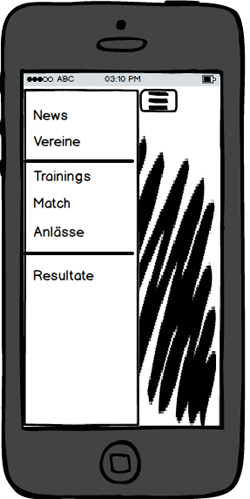
\includegraphics[scale=0.5]{images/mockups/navigation.png}
  \label{fig:mockup_navigation}
}
\subfigure[Einstellungen]{
  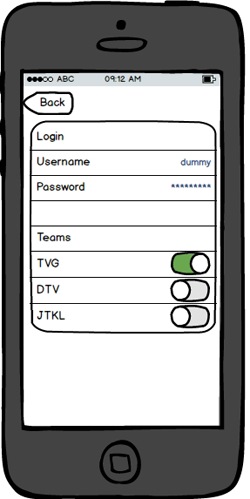
\includegraphics[scale=0.5]{images/mockups/settings.png}
  \label{fig:mockup_settings}
}
\label{fig:mockup_setting}
\caption{Navigation und Einstellungen}
\end{figure}

\newpage
\FloatBarrier
\subsubsection{Berichte}\label{mockup_news}
Als Startseite sollte eine Seite gewählt werden, die etwas Aktuelles anzeigt, somit fiel die Entscheidung auf die Seite mit den Berichten.
\begin{figure}[ht]
\centering
\subfigure[Berichte Übersicht]{
  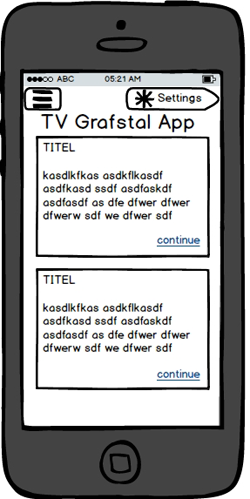
\includegraphics[scale=0.5]{images/mockups/news.png}
  \label{fig:mockup_news_list}
}
\subfigure[Bericht Details]{
  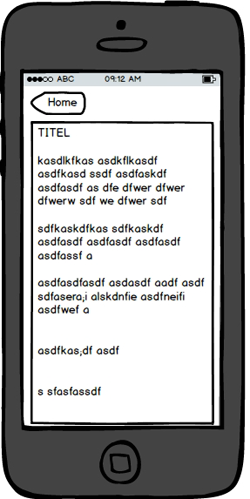
\includegraphics[scale=0.5]{images/mockups/news_detail.png}
  \label{fig:mockup_news_detail}
}
\label{fig:mockup_news}
\caption{Berichte}
\end{figure}

\FloatBarrier
\subsubsection{Vereine}\label{mockup_vereine}
Die Überlegungen zur Gestaltung der Informationen der Vereine sahen so aus:
\begin{figure}[ht]
\centering
\subfigure[Vereine]{
  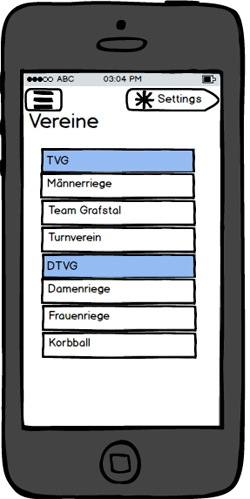
\includegraphics[scale=0.5]{images/mockups/vereine.png}
  \label{fig:mockup_vereine}
}
\subfigure[Verein Details]{
  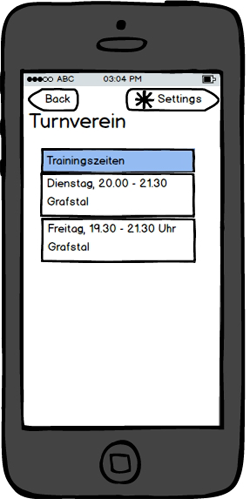
\includegraphics[scale=0.5]{images/mockups/verein_detail.png}
  \label{fig:mockup_verein_detail}
}
\label{fig:mockup_verein}
\caption{Vereine}
\end{figure}

\FloatBarrier
\subsubsection{Veranstaltungen}\label{mockup_singingobjects}
Die verschiedenen Übersichten und Detailsichten der Veranstaltungen sollten ursprünglich so aussehen:
\begin{figure}[ht]
\centering
\subfigure[Anlässe]{
  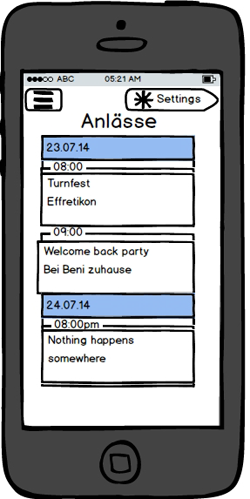
\includegraphics[scale=0.5]{images/mockups/events.png}
  \label{fig:mockup_events}
}
\subfigure[Anlass Details]{
  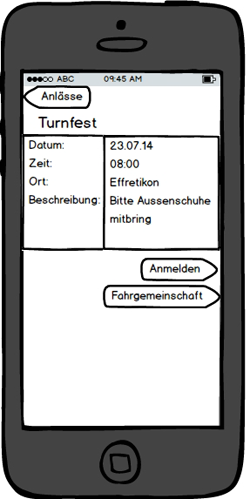
\includegraphics[scale=0.5]{images/mockups/event_detail.png}
  \label{fig:mockup_event_detail}
}
\label{fig:mockup_event}
\caption{Anlässe}
\end{figure}

\begin{figure}[ht]
\centering
\subfigure[Matches]{
  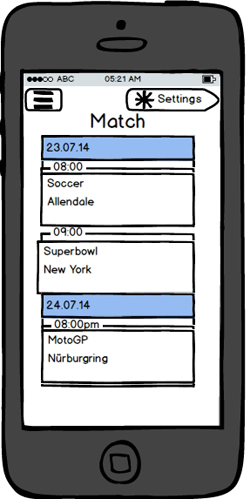
\includegraphics[scale=0.5]{images/mockups/matches.png}
  \label{fig:mockup_matches}
}
\subfigure[Match Details]{
  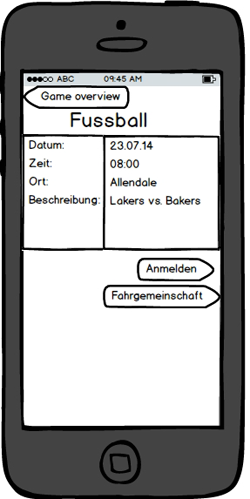
\includegraphics[scale=0.5]{images/mockups/match_detail.png}
  \label{fig:mockup_match_detail}
}
\label{fig:mockup_match}
\caption{Matches}
\end{figure}

\begin{figure}[ht]
\centering
\subfigure[Trainings]{
  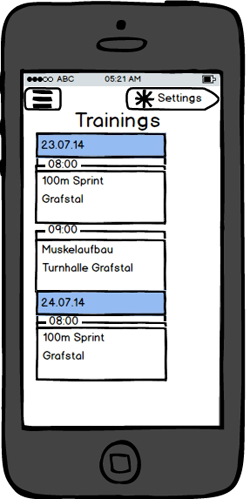
\includegraphics[scale=0.5]{images/mockups/trainings.png}
  \label{fig:mockup_trainings}
}
\subfigure[Training Details]{
  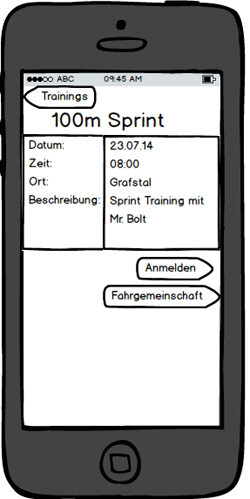
\includegraphics[scale=0.5]{images/mockups/training_detail.png}
  \label{fig:mockup_training_detail}
}
\label{fig:mockup_training}
\caption{Trainings}
\end{figure}

\FloatBarrier
\subsubsection{Resultate}\label{mockup_results}
Das \glossarmark{Mockup} für die Darstellung der Resultate sah eine veranstaltungsspezifische Darstellung vor, wurde dann im späteren Verlauf des Projektes auf eine personenspezifische Übersicht abgeändert. Diese Ansicht war kein Use Case der \glossarmark{Stakeholder} und wurde als möglicher \glossarmark{Begeisterungsfaktor} vom Entwickler hinzugefügt.
\begin{figure}[h]
\centering
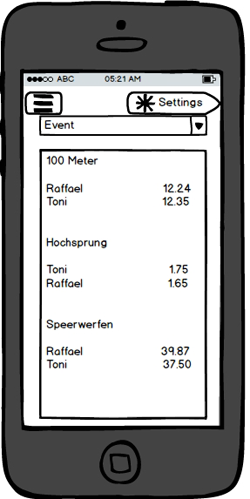
\includegraphics[scale=0.5]{images/mockups/results.png}
\caption{Resultate}
\label{fig:mockup_results}
\end{figure}

\newpage
\FloatBarrier
\subsubsection{Fahrgemeinschaften}\label{mockups_carpools}
Eine der wichtigsten Ansichten, die zu diesem Zeitpunkt nicht auf der Webseite existierte, war jene der Fahrgemeinschaft. An diesem Punkt wurden schon die ersten Überlegungen getroffen, welche Informationen für eine Fahrgemeinschaft relevant sind.
\begin{figure}[ht]
\centering
\subfigure[Fahrgemeinschafen]{
  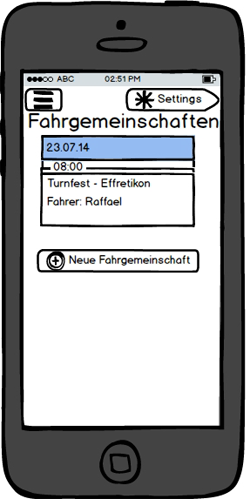
\includegraphics[scale=0.5]{images/mockups/carpools.png}
  \label{fig:mockup_carpools}
}
\subfigure[Fahrgemeinschaft Details]{
  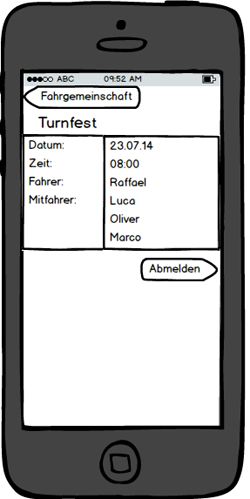
\includegraphics[scale=0.5]{images/mockups/carpool_detail.png}
  \label{fig:mockup_carpool_detail}
}
\label{fig:mockup_carpool}
\caption{Fahrgemeinschaften}
\end{figure}

\begin{figure}[h]
\centering
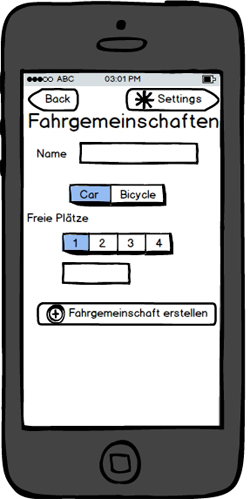
\includegraphics[scale=0.5]{images/mockups/carpool_add.png}
\caption{Fahrgemeinschaft erstellen}
\label{fig:mockup_add_carpool}
\end{figure}

\newpage
\subsection{Anforderungen}\label{anforderungen}
Alle Anforderungen wurden anhand der folgenden Vorlage (siehe Tabelle \ref{table:req_template}) erfasst. Diese Vorlage basiert auf Angaben von \cite{req_eng_book} und wurde mit eigenen Attributen erweitert.

\begin{table}[ht]
\centering
  \begin{tabular}{ l | p{8cm} }
	\hline
	\rowcolor{gray}
	\textbf{ID}			&	Eindeutiger Identifikator\\ \hline
	\textbf{Priorität} 		&	Must, Should, Nice to have\\ \hline
	\textbf{Anforderungstyp}	&	Funktionale Anforderung, Qualitätsanforderung, Randbedingung\\ \hline
	\textbf{Name} 			&	Eindeutiger, charakterisierender Name\\ \hline
	\textbf{Use Case} 		&	Referenz zum zugehörigen Use Case\\ \hline
	\textbf{Beschreibung} 	&	Beschreibung der Anforderung\\ \hline
	\textbf{Begründung} 		&	Bedeutung der Anforderung für das geplante System\\ \hline
	\textbf{Akzeptanz Kriterium}	&	Messbare Abnahmekriterien\\ \hline
	\textbf{Abhängigkeiten} 	&	Referenz zu anderen Anforderungen\\ \hline
	\textbf{Antragssteller} 	&	\glossarmark{Stakeholder}, der um diese Anforderung bittet\\ \hline
	\textbf{Risiken}	 	&	Weisst auf allfällige Risiken betreffend der Anforderungen hin
  \end{tabular}
   \caption{Vorlage für Anforderungen}\label{table:req_template}
\end{table}


Die Beschreibung der Anforderungen wurden zusätzlich mit einer Satzschablone (siehe Abbildung \ref{fig:satzschablone}) aus \cite{req_eng_book} erstellt. Dies hat den Vorteil, dass die Anforderungen normiert und exakt erfasst werden.
\begin{figure}[h]
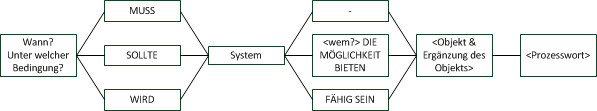
\includegraphics{images/anforderungen/satzschablone.png}
\caption{Satzschablone}
\label{fig:satzschablone}
\end{figure}
\FloatBarrier
Die Abstufungen \emph{muss}, \emph{sollte} und \emph{wird} werden verwendet um die Wichtigkeit der Anforderungen auszudrücken.

\newpage
\FloatBarrier
\subsubsection{Funktionale Anforderungen}\label{func_anforderungen}

\begin{table}[ht]
\centering
  \begin{tabular}{ l | p{8cm} }
	\hline
	\rowcolor{gray}
	\textbf{ID} 			&	\textbf{RE-F1}\\ \hline
	\textbf{Priorität} 		&	Must\\ \hline
	\textbf{Anforderungstyp}	&	Funktionale Anforderung\\ \hline
	\textbf{Name} 			&	Login Möglichkeit bei der Mobile App\\ \hline
	\textbf{Use Case} 		&	-\\ \hline
	\textbf{Beschreibung} 	&	Falls ein Mitglied vom Turnverein auf der Homepage registriert ist, muss das System dem besagten Mitglied die Möglichkeit bieten sich über ein Formular am Backend anzumelden.\\ \hline
	\textbf{Begründung} 		&	Einige Informationen dürfen nur für Mitglieder zugänglich
					gemacht werden. Zusätzlich vereinfacht es das Anmelden, Erstellen
					und Abrufen von benutzerspezifischen Daten\\ \hline
	\textbf{Akzeptanz Kriterium}	&	\begin{enumerate}
					\item Bei bekanntem Username und Passwort muss es dem Mitglied möglich sein, sich beim Backend anzumelden und dann erweiterte	Möglichkeiten und Informationen zu erhalten.
					\item Falls ein unbekannter Username oder das falsche Passwort eingegeben wurden kommt eine entsprechende Fehlermeldung.
					\end{enumerate}
					\\ \hline
	\textbf{Abhängigkeiten} 	&	-\\ \hline
	\textbf{Antragssteller} 	&	Dominic Keller (aktive Mitglieder (U30))\\ \hline
	\textbf{Risiken}	 	&	Falls diese Anforderung nicht erfolgreich implementiert werden kann, gibt es Schwierigkeiten bei sehr vielen anderen Anforderungen.
  \end{tabular}
   \caption{Anforderung RF-F1}\label{table:req_1}
\end{table}

\begin{table}[ht]
\centering
  \begin{tabular}{ l | p{8cm} }
	\hline
	\rowcolor{gray}
	\textbf{ID} 			&	\textbf{RE-F2}\\ \hline
	\textbf{Priorität} 		&	Must\\ \hline
	\textbf{Anforderungstyp}	&	Funktionale Anforderung\\ \hline
	\textbf{Name} 			&	Fahrgemeinschaft erstellen\\ \hline
	\textbf{Use Case} 		&	\nameref{table:use_case_1}\\ \hline
	\textbf{Beschreibung} 	&	Falls das Mitglied angemeldet ist, muss das System dem besagten Mitglied die Möglichkeit bieten über ein Formular eine neue Fahrgemeinschaft zu eröffnen.\\ \hline
	\textbf{Begründung} 		&	Seit einiger Zeit wird vermehrt der Vereins-Chat mit endlosen Diskussionen für Fahrgemeinschaftsorganisationen verwendet, was einige Mitglieder stört und auch nicht der Sinn und Zweck dieses Chats ist. Jedes Mitglied sollte über die App die Möglichkeit haben seine Fahrdienste zur Verfügung zu stellen.\\ \hline
	\textbf{Akzeptanz Kriterium}	&	\begin{enumerate}
					\item Das angemeldete Mitglied kann eine Fahrgemeinschaft eröffnen
					\item Bei ungültigen oder nicht ausreichenden Informationen kommt eine entsprechende Fehlermeldung
					\end{enumerate}
					\\ \hline
	\textbf{Abhängigkeiten} 	&	\nameref{table:req_1}\\ \hline
	\textbf{Antragssteller} 	&	Marco Mathe (Vorstand)\\ \hline
	\textbf{Risiken}	 	&	-
  \end{tabular}
   \caption{Anforderung RF-F2}\label{table:req_2}
\end{table}

\begin{table}[ht]
\centering
  \begin{tabular}{ l | p{8cm} }
	\hline
	\rowcolor{gray}
	\textbf{ID} 			&	\textbf{RE-F3}\\ \hline
	\textbf{Priorität} 		&	Must\\ \hline
	\textbf{Anforderungstyp}	&	Funktionale Anforderung\\ \hline
	\textbf{Name} 			&	Übersicht über Fahrgemeinschaft\\ \hline
	\textbf{Use Case} 		&	\nameref{table:use_case_2}\\ \hline
	\textbf{Beschreibung} 	&	Falls das Mitglied angemeldet ist und eine Fahrgemeinschaft im System besteht, muss das System dem besagten Mitglied die Möglichkeit bieten, eine Liste aller aktuellen Fahrgemeinschaften anzeigen zu lassen.\\ \hline
	\textbf{Begründung} 		&	Das Mitglied benötigt eine Übersicht der aktuellen Fahrgemeinschaften, damit es sich für eine entscheiden kann.\\ \hline
	\textbf{Akzeptanz Kriterium}	&	\begin{enumerate}
					\item Das angemeldete Mitglied kann die Fahrgemeinschaften anzeigen lassen
					\item Das angemeldete Mitglied sieht einen Hinweis, falls es keine Fahrgemeinschaften gibt
					\end{enumerate}
					\\ \hline
	\textbf{Abhängigkeiten} 	&	\nameref{table:req_1}, \nameref{table:req_2}\\ \hline
	\textbf{Antragssteller} 	&	Marco Mathe (Vorstand)\\ \hline
	\textbf{Risiken}	 	&	Falls nur die \nameref{table:req_2} implementiert wird und diese nicht, ist das Fahrgemeinschaft-System nicht funktionsfähig
  \end{tabular}
   \caption{Anforderung RF-F3}\label{table:req_3}
\end{table}

\begin{table}[ht]
\centering
  \begin{tabular}{ l | p{8cm} }
	\hline
	\rowcolor{gray}
	\textbf{ID} 			&	\textbf{RE-F4}\\ \hline
	\textbf{Priorität} 		&	Must\\ \hline
	\textbf{Anforderungstyp}	&	Funktionale Anforderung\\ \hline
	\textbf{Name} 			&	Fahrgemeinschaft beitreten\\ \hline
	\textbf{Use Case} 		&	\nameref{table:use_case_3}\\ \hline
	\textbf{Beschreibung} 	&	Falls das Mitglied angemeldet ist, eine Fahrgemeinschaft im System besteht, das besagte Mitglied noch nicht beigetreten ist und die Fahrgemeinschaft noch Kapazität aufweist, muss das System dem besagten Mitglied die Möglichkeit bieten, sich über einen Knopf bei einer Fahrgemeinschaft einzutragen.\\ \hline
	\textbf{Begründung} 		&	Damit die Fahrgemeinschaften auch funktionieren, muss es den Mitgliedern möglich sein, sich selbständig bei den Fahrgemeinschaften einzutragen.\\ \hline
	\textbf{Akzeptanz Kriterium}	&	\begin{enumerate}
					\item Das angemeldete Mitglied kann einer Fahrgemeinschaft beitreten
					\item Das angemeldete Mitglied kann einer Fahrgemeinschaft nicht erneut beitreten
					\item Das angemeldete Mitglied erhält eine Fehlermeldung falls die Fahrgemeinschaft keine Kapazität mehr aufweist
					\end{enumerate}
					\\ \hline
	\textbf{Abhängigkeiten} 	&	\nameref{table:req_1}, \nameref{table:req_2}, \nameref{table:req_3}\\ \hline
	\textbf{Antragssteller} 	&	Marco Mathe (Vorstand)\\ \hline
	\textbf{Risiken}	 	&	Falls nur die \nameref{table:req_2} und \nameref{table:req_3} implementiert werden und diese nicht, ist das Fahrgemeinschaft-System nicht funktionsfähig
  \end{tabular}
   \caption{Anforderung RF-F4}\label{table:req_4}
\end{table}

\begin{table}[ht]
\centering
  \begin{tabular}{ l | p{8cm} }
	\hline
	\rowcolor{gray}
	\textbf{ID} 			&	\textbf{RE-F5}\\ \hline
	\textbf{Priorität} 		&	Should\\ \hline
	\textbf{Anforderungstyp}	&	Funktionale Anforderung\\ \hline
	\textbf{Name} 			&	Anmelden an Vereinsanlässe\\ \hline
	\textbf{Use Case} 		&	\nameref{table:use_case_4}\\ \hline
	\textbf{Beschreibung} 	&	Falls das Mitglied angemeldet ist, ein Anlass im System besteht und das besagte Mitglied noch nicht angemeldet ist, sollte das System dem besagten Mitglied die Möglichkeit bieten, sich über einen Knopf für den Anlass anzumelden.\\ \hline
	\textbf{Begründung} 		&	Die Anmeldequote der Mitglieder ist nicht so hoch wie erwünscht, durch das Anbieten der Anmelde-Möglichkeit über das App soll das Anmelden vereinfacht und die Anmeldequote erhöht werden.\\ \hline
	\textbf{Akzeptanz Kriterium}	&	\begin{enumerate}
					\item Das angemeldete Mitglied kann sich für einen Anlass anmelden
					\item Das angemeldete Mitglied kann sich für einen Anlass nicht erneut anmelden
					\end{enumerate}
					\\ \hline
	\textbf{Abhängigkeiten} 	&	\nameref{table:req_1}, \nameref{table:req_2}, \nameref{table:req_3}\\ \hline
	\textbf{Antragssteller} 	&	Dominic Keller (aktive Mitglieder (U30))\\ \hline
	\textbf{Risiken}	 	&	-
  \end{tabular}
   \caption{Anforderung RF-F5}\label{table:req_5}
\end{table}

\begin{table}[ht]
\centering
  \begin{tabular}{ l | p{8cm} }
	\hline
	\rowcolor{gray}
	\textbf{ID} 			&	\textbf{RE-F6}\\ \hline
	\textbf{Priorität} 		&	Must\\ \hline
	\textbf{Anforderungstyp}	&	Funktionale Anforderung\\ \hline
	\textbf{Name} 			&	Informationen über Vereinsanlässe\\ \hline
	\textbf{Use Case} 		&	\nameref{table:use_case_5}\\ \hline
	\textbf{Beschreibung} 	&	Falls ein Anlass im System ist, muss das System dem Benutzer der App die Möglichkeit bieten, Informationen über Vereinsanlässe zu erhalten.\\ \hline
	\textbf{Begründung} 		&	Über die App kann man die Informationen schnell und einfach abrufen, somit sollte den Anlässen mehr Beachtung geschenkt werden.\\ \hline
	\textbf{Akzeptanz Kriterium}	&	\begin{enumerate}
					\item Der Benutzer erhält informationen über den ausgewählten Anlass
					\item Der Benutzer sieht einen Hinweis, falls keine Anlässe vorhanden sind
					\end{enumerate}
					\\ \hline
	\textbf{Abhängigkeiten} 	&	-\\ \hline
	\textbf{Antragssteller} 	&	Ivan Sebastiano (Vorstand)\\ \hline
	\textbf{Risiken}	 	&	-
  \end{tabular}
   \caption{Anforderung RF-F6}\label{table:req_6}
\end{table}

\begin{table}[ht]
\centering
  \begin{tabular}{ l | p{8cm} }
	\hline
	\rowcolor{gray}
	\textbf{ID} 			&	\textbf{RE-F7}\\ \hline
	\textbf{Priorität} 		&	Must\\ \hline
	\textbf{Anforderungstyp}	&	Funktionale Anforderung\\ \hline
	\textbf{Name} 			&	Erweiterte Informationen über Vereinsanlässe\\ \hline
	\textbf{Use Case} 		&	\nameref{table:use_case_5}\\ \hline
	\textbf{Beschreibung} 	&	Falls das Mitglied angemeldet ist und ein Anlass im System besteht, sollte das System dem besagten Mitglied die Möglichkeit bieten, zusätzliche Informationen über den Anlass zu erhalten.\\ \hline
	\textbf{Begründung} 		&	Einige Informationen (z. B. Anmelde-Listen) sind aus Datenschutz- oder anderen Gründen nicht für alle Nutzer der App bestimmt und sollten nur angemeldeten Mitgliedern angezeigt werden.\\ \hline
	\textbf{Akzeptanz Kriterium}	&	\begin{enumerate}
					\item Das angemeldete Mitglied sieht die erweiterten Informationen zum Anlass
					\item Nicht angemeldete Mitglieder sehen die erweiterten Informationen zum Anlass nicht
					\end{enumerate}
					\\ \hline
	\textbf{Abhängigkeiten} 	&	\nameref{table:req_1}, \nameref{table:req_6}\\ \hline
	\textbf{Antragssteller} 	&	Ivan Sebastiano (Vorstand)\\ \hline
	\textbf{Risiken}	 	&	-
  \end{tabular}
   \caption{Anforderung RF-F7}\label{table:req_7}
\end{table}

\begin{table}[ht]
\centering
  \begin{tabular}{ l | p{8cm} }
	\hline
	\rowcolor{gray}
	\textbf{ID} 			&	\textbf{RE-F8}\\ \hline
	\textbf{Priorität} 		&	Must\\ \hline
	\textbf{Anforderungstyp}	&	Funktionale Anforderung\\ \hline
	\textbf{Name} 			&	Informationen über Vereine und Riegen\\ \hline
	\textbf{Use Case} 		&	\nameref{table:use_case_6}\\ \hline
	\textbf{Beschreibung} 	&	Das System muss dem Benutzer der App die Möglichkeit bieten, Informationen über die verschiedenen Vereine und Riegen zu erhalten.\\ \hline
	\textbf{Begründung} 		&	Die App ist nicht nur für die Mitglieder des Vereins sondern auch für Aussenstehende und sollte auch zu Werbezwecken dienen. Jeder kann aktuelle Trainingszeiten und Inhalte der Trainings anschauen und erhält Kontaktinformationen.\\ \hline
	\textbf{Akzeptanz Kriterium}	&	\begin{enumerate}
					\item Der Benutzer erhält Informationen über die verschiedenen Vereine und Riegen
					\end{enumerate}
					\\ \hline
	\textbf{Abhängigkeiten} 	&	-\\ \hline
	\textbf{Antragssteller} 	&	Ivan Sebastiano (Vorstand)\\ \hline
	\textbf{Risiken}	 	&	-
  \end{tabular}
   \caption{Anforderung RF-F8}\label{table:req_8}
\end{table}

\begin{table}[ht]
\centering
  \begin{tabular}{ l | p{8cm} }
	\hline
	\rowcolor{gray}
	\textbf{ID} 			&	\textbf{RE-F9}\\ \hline
	\textbf{Priorität} 		&	Must\\ \hline
	\textbf{Anforderungstyp}	&	Funktionale Anforderung\\ \hline
	\textbf{Name} 			&	Aktuellen Berichte\\ \hline
	\textbf{Use Case} 		&	\nameref{table:use_case_6}\\ \hline
	\textbf{Beschreibung} 	&	Das System muss dem Benutzer der App die Möglichkeit bieten, aktuellen Berichte von den einzelnen Anlässen oder Vereinen lesen zu können.\\ \hline
	\textbf{Begründung} 		&	Die App ist nicht nur für die Mitglieder des Vereins sondern auch für Aussenstehende und sollte auch zu Werbezwecken dienen. In den Berichten wird über aktuelle Anlässe und Geschehnisse geschrieben, ganz nach dem Motto 'Tue gutes und sprich darüber'.\\ \hline
	\textbf{Akzeptanz Kriterium}	&	\begin{enumerate}
					\item Der Benutzer kann die aktuellen Berichte lesen
					\end{enumerate}
					\\ \hline
	\textbf{Abhängigkeiten} 	&	-\\ \hline
	\textbf{Antragssteller} 	&	Dominic Keller (aktive Mitglieder (U30))\\ \hline
	\textbf{Risiken}	 	&	-
  \end{tabular}
   \caption{Anforderung RF-F9}\label{table:req_9}
\end{table}

\begin{table}[ht]
\centering
  \begin{tabular}{ l | p{8cm} }
	\hline
	\rowcolor{gray}
	\textbf{ID} 			&	\textbf{RE-F10}\\ \hline
	\textbf{Priorität} 		&	Nice to have\\ \hline
	\textbf{Anforderungstyp}	&	Funktionale Anforderung\\ \hline
	\textbf{Name} 			&	Push-Nachrichten versenden\\ \hline
	\textbf{Use Case} 		&	-\\ \hline
	\textbf{Beschreibung} 	&	Falls das Mitglied angemeldet ist, Push-Nachrichten zugelassen werden und eine solche vom Backend versendet wurde, sollte das System dem besagten Mitglied eine Push Notification zustellen.\\ \hline
	\textbf{Begründung} 		&	Trainingsverantwortliche und Vorstandsmitglieder können die Mitglieder mit Push-Nachrichten schneller über kurzfristige Änderungen informieren.\\ \hline
	\textbf{Akzeptanz Kriterium}	&	\begin{enumerate}
					\item Das angemeldete Mitglied erhält die Push-Nachrichten
					\end{enumerate}
					\\ \hline
	\textbf{Abhängigkeiten} 	&	\nameref{table:req_1}\\ \hline
	\textbf{Antragssteller} 	&	Oliver Zimmermann (Trainingsverantwortliche)\\ \hline
	\textbf{Risiken}	 	&	-
  \end{tabular}
   \caption{Anforderung RF-F10}\label{table:req_10}
\end{table}

\newpage
\FloatBarrier
\subsubsection{Qualitätsanforderung}\label{non_func_anforderungen}

\begin{table}[ht]
\centering
  \begin{tabular}{ l | p{8cm} }
	\hline
	\rowcolor{gray}
	\textbf{ID} 			&	\textbf{RE-NF1}\\ \hline
	\textbf{Priorität} 		&	Must\\ \hline
	\textbf{Anforderungstyp}	&	Qualitätsanforderung\\ \hline
	\textbf{Name} 			&	Unterstützung von Android\\ \hline
	\textbf{Use Case} 		&	-\\ \hline
	\textbf{Beschreibung} 	&	Das System muss fähig sein, auf Android Geräten zu laufen.\\ \hline
	\textbf{Begründung} 		&	Die Statistik der aktuellen Homepage zeigt, dass über 50\% der Zugriffe über Mobiltelefone und Tablet von Android Plattformen stammen.\\ \hline
	\textbf{Akzeptanz Kriterium}	&	\begin{enumerate}
					\item Ein Nutzer mit einem Android Mobiltelefon kann die App öffnen und verwenden
					\end{enumerate}
					\\ \hline
	\textbf{Abhängigkeiten} 	&	-\\ \hline
	\textbf{Antragssteller} 	&	Dominic Keller (aktive Mitglieder (U30))\\ \hline
	\textbf{Risiken}	 	&	-
  \end{tabular}
   \caption{Qualitätsanforderung RF-NF1}\label{table:req_nf_1}
\end{table}

\begin{table}[ht]
\centering
  \begin{tabular}{ l | p{8cm} }
	\hline
	\rowcolor{gray}
	\textbf{ID} 			&	\textbf{RE-NF2}\\ \hline
	\textbf{Priorität} 		&	Must\\ \hline
	\textbf{Anforderungstyp}	&	Qualitätsanforderung\\ \hline
	\textbf{Name} 			&	Unterstützung von iOS\\ \hline
	\textbf{Use Case} 		&	-\\ \hline
	\textbf{Beschreibung} 	&	Das System muss fähig sein, auf iOS Geräten zu laufen.\\ \hline
	\textbf{Begründung} 		&	Die Statistik der aktuellen Homepage zeigt, dass gut 43\% der Zugriffe über Mobiltelefone und Tablet von iOS Plattformen stammen.\\ \hline
	\textbf{Akzeptanz Kriterium}	&	\begin{enumerate}
					\item Ein Nutzer mit einem iPhone kann die App öffnen und verwenden
					\end{enumerate}
					\\ \hline
	\textbf{Abhängigkeiten} 	&	-\\ \hline
	\textbf{Antragssteller} 	&	Marco Mathe (Vorstand)\\ \hline
	\textbf{Risiken}	 	&	-
  \end{tabular}
   \caption{Qualitätsanforderung RF-NF2}\label{table:req_nf_2}
\end{table}



%%%%%%%%%%%%%%%%%%%%%%%%%%%%%%%%%%%%%%%%%%%%%%%%%%%%%%%%%%%%%%%%%
%
% Project     : Turnverein App
% Title       : 
% File        : architektur.tex Rev. 00
% Date        : 07.07.14
% Author      : Raffael Santschi
%
%%%%%%%%%%%%%%%%%%%%%%%%%%%%%%%%%%%%%%%%%%%%%%%%%%%%%%%%%%%%%%%%%

\chapter{Architektur}\label{chap.architektur}
In diesem Kapitel wird auf die ganze Strukur und die Architektur des Backends und des Apps eingegangen. Die Architektur legt die Grundlage für die Umsetzung und sollte mit Bedacht festgelegt werden.

\section{Übersicht}\label{architektur_uebersicht}
Die Systemumgebung (siehe Abbildung \ref{fig:system_scope}) besteht aus einem Webserver, auf welchem das Backend, die Webseite und neu auch die API-Schnitstelle für das App läuft. Die Web-Schnitstelle für Funktioninäre wird in diesem Bild seperat aufgeführt, da sie viel mehr Funktionen bietet, als für normale Mitglieder und Nicht-Mitglieder, sie ist jedoch über die gleiche Webseite ansprechbar. Das RESTful API, mit welcher das App kommuniziert, beherrscht nur die in den Anforderungen benötigten Funktionen.
\begin{figure}[h]
\centering
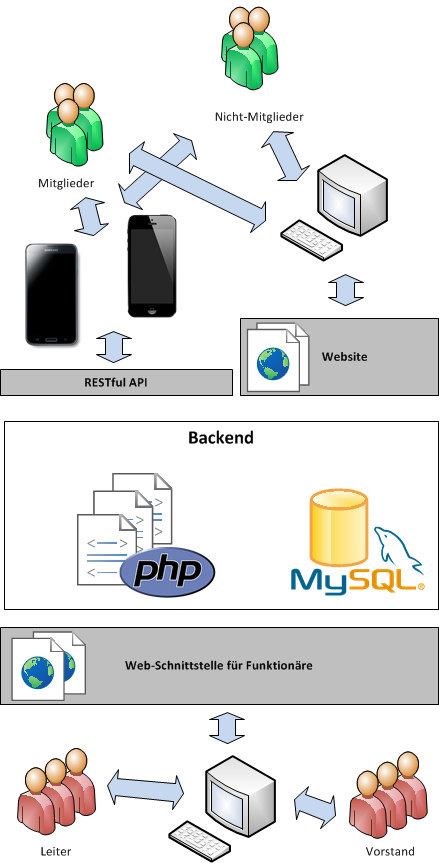
\includegraphics[scale=0.5]{images/visio/SystemScope.png}
\caption{System Übersicht}
\label{fig:system_scope}
\end{figure}

\section{Backend}\label{arch_backend}
Im PHP Backend wird seit diesem Projekt Doctrine (siehe \cite{doctrine} und \cite{dunglas2013persistence}) als Objektrelationaler Mapper (ORM) verwendet. Ein ORM hat den Vorteil, dass man mit einer Konfiguration Tabellen mit Objekten verknüpfen kann und somit viel Arbeit im Bezug auf die Datenbankkommunikation wegfällt. Ein Nachteil bei einem ORM kann sein, dass man Funktionen, welche Datenbank spezfisch sind, nicht verwenden kann oder diese nur mit grossem Aufwand. Doctrine bietet auch Locking-Mechanismen, welche in diesem Projekt benötigt werden. Es gibt die Möglichkeit die Entity-Konfiguration in ein File auszulagern oder mit Annotationen direkt im Objekt zu erfassen, zweiteres ist in diesem Projekt der Fall. 

\subsection{Locking}
Das Problem bei einer Fahrgemeinschaftsverwaltung ist, dass man eine beschränkte Anzahl an Plätzen hat. Wenn man jetzt davon ausgeht, dass es noch drei freie Plätze hat und vier Mitglieder gleichzeitig auf den Anmelde-Knopf klicken, wäre die Fahrgemeinschaft plötzlich überbucht. Das Szenario ist etwas unwahrscheinlich, jedoch werden die Fahrgemeinschaften immer sehr Zeitnah an der Veranstaltung erstellt und somit ist die Zeitspanne, in der sich Mitglieder anmelden, nicht sehr gross. Eine Überbuchte Fahrgemeinschaft führt zu Ärger, welcher durch ein gezieltes Locking einfach vermieden werden kann.\\

Es gibt zwei verschiedene Varianten von Locking, das optimistische Locking und das pessimistische Locking. Das optimistische Locking funktioniert so, dass eine Zeitstempfel oder eine Versionsnummer\footnote{besser Variante, da der Zeitstempfel bei sehr schnellen und vielen Transaktionen und je nach Auflösungsgenauigkeit fehler verursachen könnte} abgespeichert wird, wenn man das Objekt lädt. Wenn man nun etwas verändern möchte, wird diese Versionsnummer mitgegeben und geprüft, ob sich die Version seit diesem Zeitpunkt bereits verändert hat. Das pessimistische Locking wird mittels einem Lock, sei dass einem zeilenbasierten oder tabellenbasierten Lock, und einer Transaktion umgeben.\\

Die Implementation in diesem Projekt sieht für den User wie ein optimstisches Locking aus, alle vier Mitglieder, aus dem Beispiel oben, sehen den Anmelde-Knopf und einer erhält am Schluss die Fehlermeldung, dass es keinen Platz mehr hat. Im Backend ist es jedoch mit einem pessimistischen Locking auf Zeilenebene gelöst. Die Transaktion wird eröffnet, die Zeile wird gelockt, der Request wird überprüft, der Eintrag wird gespeichert und danach wird die Zeile mit dem Beenden der Transaktion wieder freigegeben. Um diesen Vorgang etwas besser zu veranschaulichen wurde ein Sequenzdiagramm (siehe Abbildung \ref{fig:locking_verfahren}) erstellt, dies wurde anhand der Vorlage in \cite{soft_arch_book}.

\begin{figure}[h]
\centering
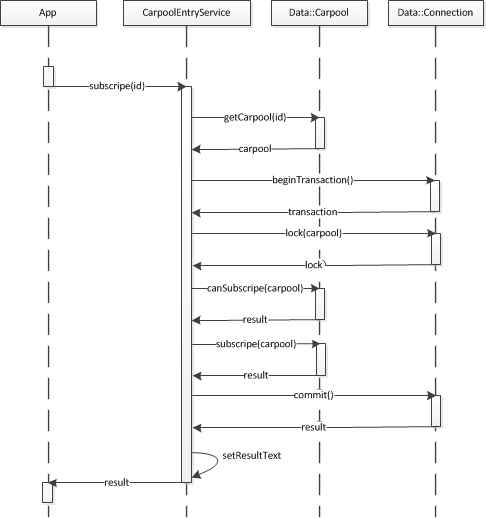
\includegraphics[scale=0.5]{images/visio/locking_verfahren.png}
\caption{Sequenzdiagramm - Locking Verfahren}
\label{fig:locking_verfahren}
\end{figure}

\FloatBarrier
\subsection{API}
Das App enthält so gut wie keine Daten, sondern holt diese immer von dem Backend. Dazu wurde ein RESTful API erstellt, welches JavaScript Object Notation-Objekte (JSON-Objekte) zurück liefert. Das API funktioniert nach dem De-facto-Standard (siehe \cite{wiki_restful}). Bei einem Listen-Aufruf ohne Einträge liefert es eine leere Liste zurück, wenn ein spezifisches Objekt abgerufen wird, liefert es 'null' zurück. Bei Aktionen wird ein JSON-Objekt mit den Attributen 'success' und 'error\_message' zurück gegeben.\\

Das API hat eine Versionsnummer in der URL, damit kann sichergestellt werden, dass ältere Versionen von der App immer noch lauffähig sind, wenn etwas an der Schnittstelle geändert wird. Dieser Punkt ist sehr wichtig, da man den Usern nicht vorschreiben kann, wann und ob sie ihr App updaten.

\section{Lösungsvarianten}\label{loesungsvarianten}
Es gibt verschiedene wege ein App zu entwickeln und jede hat seine Vor- und Nachteile. In diesem Abschnitt werden drei verschiedenen Methoden miteinander verglichen und die beste für diesen Anwendungszweck ausgewählt.

\subsection{Native App}\label{architektur_native}
Früher gab es nur diese Variante der App Entwicklung, man musste für jede Plattform die bereitgestellte Integrated Development Environment (IDE) verwenden und die dazugehörige Sprache lernen. Bei Apple ist das XCode und Objective-C, bei Android früher Eclispe Android Development Tools (ADT) und heute Android Studio basierend auf IntelliJ beide Male mit der Programmiersprache Java. Die Vorteile sind voller Funktionsumfang und gute Unterstützung bei der Entwicklung durch die IDE's. Das führen von zwei oder mehreren seperaten Code-Sourcen ist jedoch sehr aufwendig und mühesam.

\subsection{Xamarin}\label{architektur_xamarin}
Xamarin (siehe \cite{xamarin}) ist ein sehr mächtiges Framework, welches es ermöglicht den Code der App in C\# zu schreiben und dies dann in Native Code umzuwandeln. Xamarin liefert seine eigene IDE kann aber auch in Visual Studio integriert werden Grosse Firmen wie 3M, AT\&T und HP verwenden Xamarin für ihre Apps. Der grosse Vorteil ist, dass man fast alle Funktionen einer Native App verwenden kann und dazu nur eine Sprache und eine IDE beherrschen muss. 

\subsection{Phonegap}\label{architektur_phonegapt}
Phonegap (siehe \cite{phonegap} und \cite{wargo2012phonegap}) basiert auf Cordova (siehe \cite{cordova}), ein Framework von Apache, mit welchem es möglich ist eine Webseite geschrieben in HTML und Javascript in eine Native App umzuwandeln. Phonegap bietet Javascript Plugins um die Native Funktionen wie zum Beispiel Geolocation, Kompass oder Push-Nachrichten zu benutzen. Das Framework erstellt für die gewünschte Plattform ein App mit einer Webview und fügt die nötigen Klassen für die Plugins hinzu. Ein positiver Nebeneffekt ist bei dieser Methode, dass man die Webseite auch online stellen kann und alles ausser die Plugins benutzt werden kann. Phonegap bietet im Gegensatz zu den anderen Varianten keinen Möglichkeit grafischen Benutzeroberflächen zu modelieren oder ähnliches, es kümmert sich lediglich um die Konvertierung in die verschiedenen Plattformen und stellt die Schnittstellen zu den Native Funktionen bereit. Phonegap wird oft mit einem für mobile Geräte optimiertem Framework wie zum Beispiel jQuery Mobile (siehe \cite{jquery_mobile} und \cite{reid2011jquery}) kombiniert.

\newpage
\subsection{Nutzwertanalyse}\label{architektur_nutzwertanalyse}

\subsubsection{Bewertungskriterien}\label{architektur_bewertungspunkte}

In der Nutzwertanalyse werden folgende Punkte betrachtet und nach dem angegebenen Schema bewertet und dann gewichtet. Die Kriterien sind grösstenteils aus den Softwarequalitäsmerkmalen nach \cite{iso_9126} abgeleitet.

\paragraph{Aufwand}
\begin{itemize}
	\item \textbf{Beschreibung}: Wie gross ist der geschätzte Aufwand mit dieser Methode?
	\item \textbf{Bewertung}: 1: sehr hoch, 10: sehr niedrig
	\item \textbf{Gewichtung}: 5 (Die Zeit für dieses Projekt ist beschränkt und die Entscheidung könnte zu einem Risiko werden)
\end{itemize}

\paragraph{Benutzbarkeit}
\begin{itemize}
	\item \textbf{Beschreibung}: Wie schnell hat man diese Variante erlernt? 
	\item \textbf{Bewertung}: 1: sehr langsam, 10: sehr schnell
	\item \textbf{Gewichtung}: 4 (Umso mehr Zeit für das Erlernen investiert wird, umso weniger Zeit hat man für die Implementierung)
\end{itemize}

\paragraph{Übertragbarkeit}
\begin{itemize}
	\item \textbf{Beschreibung}: Wie flexibel ist diese Variante? Kann sie auf verschiedenen Plattformen laufen? 
	\item \textbf{Bewertung}: 1: sehr spezifisch, nicht portabel, 10: sehr flexibel
	\item \textbf{Gewichtung}: 4 (Die Anforderungen geben vor, dass das App mindests auf Android und iOS laufen muss)
\end{itemize}

\paragraph{Funktionalität}
\begin{itemize}
	\item \textbf{Beschreibung}: Wie gross ist der Funktionalitätsumfang? 
	\item \textbf{Bewertung}: 1: sehr eingeschränkt, 10: sehr weit reichend
	\item \textbf{Gewichtung}: 3 (In der ersten Version der App wird noch nicht viel Funktionalität gebraucht)
\end{itemize}

\paragraph{Kosten}
\begin{itemize}
	\item \textbf{Beschreibung}: Wie viel kostet diese Lösung? 
	\item \textbf{Bewertung}: 1: sehr teuer, 10: gratis
	\item \textbf{Gewichtung}: 1 (Der Turnverein kommt für die Kosten auf und ist auch bereit etwas dafür zu bezahlen)
\end{itemize}

\newpage
\subsubsection{Bewertung}\label{architektur_bewertung}
Anhand der zuvor definierten Kriterien wurde eine Bewertung vorgenommen. Diese Bewertung ist nicht generell gültig, sie bezieht sich auf die Erfarhung des Entwicklers dieser Arbeit und das Projekt selbst.

\begin{table}[ht]
\centering
  \begin{tabular}{>{\columncolor{darkgray}} l | p{4cm} | p{4cm} | p{4cm}}
	\hline
	\rowcolor{darkgray}
	Kriterium		&	Native App	&	Xamarin 	&	Phonegap	\\ \hline
				&	
\includegraphics{images/icons/ios_android.png}	&	
\includegraphics[scale=0.25]{images/icons/xamarin.png} 	&	
\includegraphics[scale=0.25]{images/icons/phonegap_logo.jpg}	\\ \hline
	\rowcolor{gray}
	Aufwand		&	2 (10)		&	4 (20)		&	7 (35)		\\ \hline
	Begründung		&	Schon beim Support von 2 Plattformen enorm gross	
				&	C\# lernen, in Xamarin einarbeiten			
				&	jQuery Mobile erlernen, Phonegap kennen lernen	\\ \hline
	\rowcolor{gray}
	Benutzbarkeit	&	5 (20)		&	4 (16)		&	7 (28)		\\ \hline
	Begründung		&	Die IDEs sind sehr umgänglich, jedoch nicht sehr viel Erfahrung in Objectiv-C
				&	Keine Erfahrung in C\# und fast keine Erfahrung mit Visual Studio/Xamarin				
				&	Viel Erfahrung in HTML/Javascript, jedoch keine Erfahrung mit jQuery Mobile\\ \hline
	\rowcolor{gray}
	Übertragbarkeit	&	2 (8)		&	7 (28)		&	8 (32)		\\ \hline
	Begründung		&	Jede Plattform seinen eigenen Code	
				&	Einschränkung bei der Wiederverwendung von UI Code				
				&	Ausser einigen Zeilen exakt der gleiche Code	\\ \hline
	\rowcolor{gray}
	Funktionalität	&	10 (30)	&	9 (27)		&	7 (21)		\\ \hline
	Begründung		&	Alles was die Produkte bietet, kann verwendet werden		
				&	Nahezu alles kann verwendet und gemacht werden				
				&	Plugins bieten nicht den kompletten Funktionsumfang	\\ \hline
	\rowcolor{gray}
	Kosten		&	9 (9)		&	3 (3)		&	9 (9)		\\ \hline
	Begründung		&	Developer Accounts kosten, ansonsten gratis		
				&	Developer Accounts kosten, jedoch Kosten pro Plattform				
				&	Developer Accounts kosten, ansonsten gratis		\\ \hline \hline
	\rowcolor{gray}
	\textbf{Total (gewichtet)}	&	\textbf{28 (77)}	&	\textbf{27 (94)}	&	\textbf{38 (125)}	\\ \hline
  \end{tabular}
   \caption{Nutzwertanalyse - App Variante}\label{table:bewertungskriterien}
\end{table}

\FloatBarrier
\subsubsection{Fazit}\label{architektur_fazit}
Das Resultat der Nutzweranalyse ist eindeutig, die Entwicklung mittels Phonegap ist für dieses Projekt mit Abstand die beste Lösung. Die Methode hat noch weitere Vorteile, durch dass das der Code nur in eine App verpackt wird und er nicht in eine andere Sprache übersetzt wird, gibt es viel weniger Overhead. Zudem ist es möglich den Source auch in der App ohne Problem anzupassen, dass heisst, falls der Convert nicht mehr funktioniert, weil er zum Beispiel nicht mehr unterhalten wird, kann man torztdem noch weiterentwickeln und muss nicht zu erst ein Reverse Engineering machen.

\newpage
\section{Mobile App}\label{moblie_app}

Die Nuzwertanalyse \ref{architektur_nutzwertanalyse} hat gezeigt, dass die beste Methode für dieses Projekt das Phonegap Framework ist. Dies wurde im Projekt auch so umgesetzt und mit jQuery Mobile kombiniert. jQuery Mobile hat die Grundidee alle Seiten in dem selben HTML-File zu speichern, bietet jedoch auch die Möglichkeit dies in verschiedene Files aufzuteilen. In diesem Projek wurde die zweite Variante gewählt, weil damit zwar ein wenig Code-Duplikation generiert wurde, aber jede Seite einzel getest werden konnte, nur die nötigen Elemente geladen werden müssen und vorallem damit die HTML-Files übersichtlich bleiben. Die einzelnen Seiten sind sehr einfach aufgebaut, sie bestehen aus einem Header, in welchem das Menü, bzw. in Unterseiten die Back-Taste, und die Einstellungen aufgerufen werden können. Der Inhalt wird in einer ListView angezeigt. Die Daten werden über einen jeweiligen Asynchronous JavaScript and XML-Request (Ajax-Request) vom Backen abgeholt und dann in die ListView abgefüllt.\\

Von Phonegap wurden die Plugins PushNotification, für das Empfangen von Push-Nachrichten, und Device verwendet. Das PushNotification Plugin muss für Android und iOS spezifisch initialisiert werden und um herauszufinden, auf welcher Plattform das App läuft, wurde das Device Plugin verwendet. \\



 
%%%%%%%%%%%%%%%%%%%%%%%%%%%%%%%%%%%%%%%%%%%%%%%%%%%%%%%%%%%%%%%%%
%
% Project     : Turnverein App
% Title       : 
% File        : umsetzung.tex Rev. 00
% Date        : 07.07.14
% Author      : Raffael Santschi
%
%%%%%%%%%%%%%%%%%%%%%%%%%%%%%%%%%%%%%%%%%%%%%%%%%%%%%%%%%%%%%%%%%

\chapter{Umsetzung des Prototyps}\label{chap.umsetzung}
In diesem Kapitel wird kurz auf die Entwicklungsumgebung, die für dieses Projekt verwendet wurde, eingegangen. Danach wird erklärt, wie die Umsetzung des Backends und des Mobile App Prototyps durchgeführt wurde.

\section{Entwicklungsumgebung}\label{entwicklungsumgebung}
Ein Softwareprojekt benötigt immer eine gewisse Umgebung, welche die erforderlichen Funktionen erfüllt. Die Entwicklung einer App mit Hilfe von Phonegap kommt mit wenig aus und die Entwicklungsumgebung ist schnell aufgebaut.

\subsection{IDE - Integrated Development Environment}
Eine \glossarmark{IDE}, um welche man sicher nicht herum kommt, ist XCode. Sie wird benötigt um die App zu paketieren und sie direkt zur Analyse von Apple hochzuladen. Zusätzlich wurde noch Aptana Studio, welches für Webentwicklung ausgelegt ist, verwendet. Hier könnte man aber auf beliebige Alternativen umsteigen und notfalls auch mit einem gewöhnlichen Texteditor arbeiten. Die Vorteile einer \glossarmark{IDE} sind Syntax-Highlighting, -Checking und Autocompletion.

\begin{figure}[h]
\centering
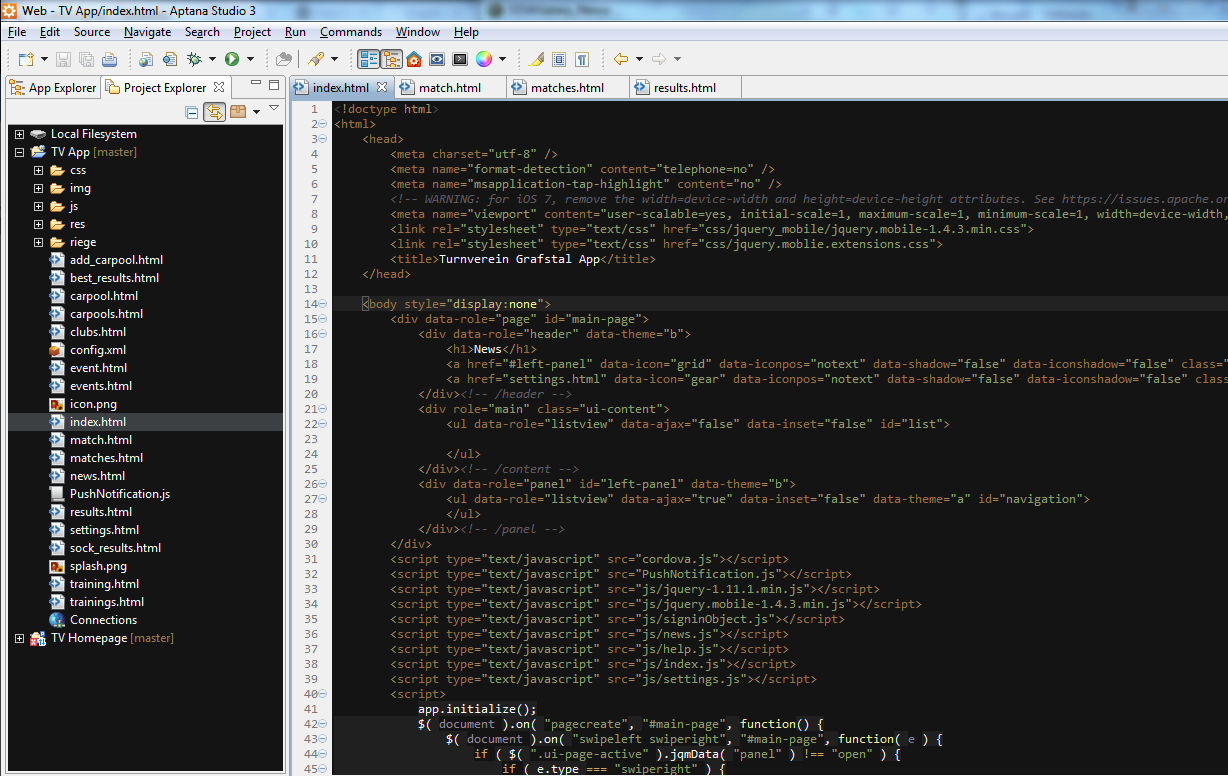
\includegraphics[scale=0.5]{images/aptana.png}
\caption{Aptana Studio}
\label{fig:aptana}
\end{figure}


\subsection{Versionierung}
Versionieriung ist in der Softwareentwicklung ein sehr wichtiges Thema, früher war das ein manueller Task, heute gibt es verschiedenste Tools, die einen dabei unterstützen. In diesem Projekt wurde git (siehe \cite{git}) verwendet, was eines der verbreitetsten Versionierungstools ist. Das Remote Repository wurde auf Github (siehe \cite{github_app}) erstellt. Es wurde geschaut, dass der Code jeden Abend auf das Repository geladen wurde, damit man auch gleich ein Backup hat.

\begin{figure}[h]
\centering
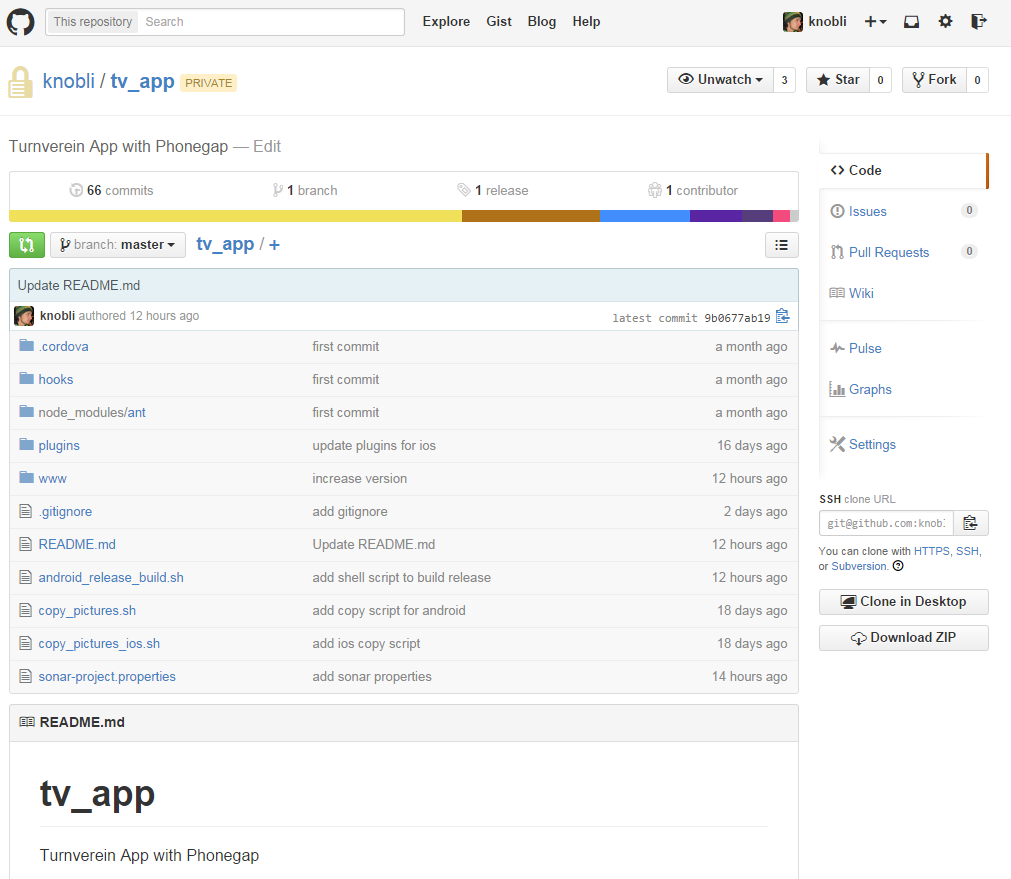
\includegraphics[scale=0.5]{images/github.png}
\caption{Github Repository}
\label{fig:github_repo}
\end{figure}

\newpage
\subsection{SDK - Software Development Kit}
Für die Entwicklung der App auf den beiden Plattformen Android und iOS wurden die dazugehörigen SDKs gebraucht, um die Applikation in einem Emulator laufen zu lassen. Vor allem bei Android, mit seinen diversen Gerätevariationen, macht das Sinn, weil man mit dem Emulator jedes beliebige Device emulieren kann.

\begin{figure}[h]
\centering
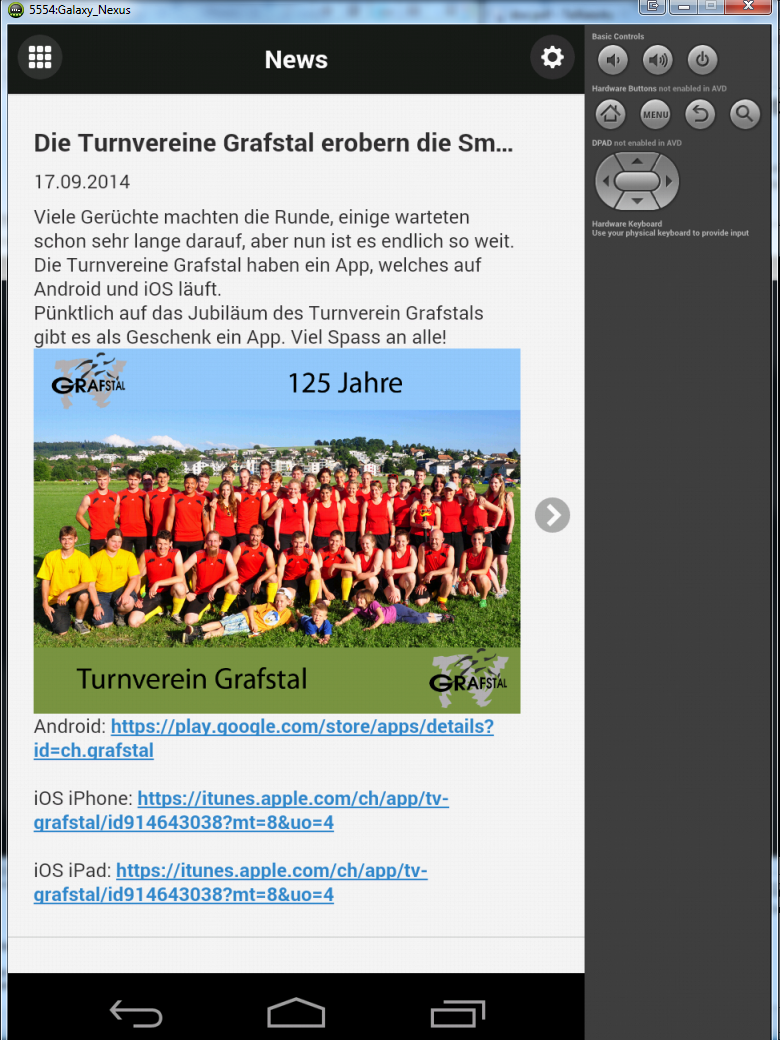
\includegraphics[scale=0.25]{images/android_emulator.png}
\caption{Android Emulator}
\label{fig:android_emulator}
\end{figure}

\FloatBarrier
\subsection{Webbrowser}
Die App wurde nicht nur auf Emulatoren getestet, sondern auch in Browsern. Dazu wurde auf Windows mit Google Chrome und auf Mac OSX mit Safari gearbeitet.

\subsection{Technische Geräte}
Push-Nachrichten können weder auf Emulatoren noch in Webbrowsern getestet werden, dafür benötigt man ein physisches Gerät. Die App wurde auf einem iPhone 4S, iPhone 5S, iPad und Samsung Ace getestet. Für die Entwicklung wurde ein Windows PC verwendet. Damit XCode benutzt werden konnte, wurde zusätzlich noch auf einem iMac gearbeitet.

\newpage
\subsection{Testen - Analysieren}
Zusätzlich zu den manuellen Tests an Geräten und  Emulatoren wurden auch automatisierte Tests und Analysen durchgeführt. Für die automatisierten Tests im Backend wurde PHPunit (siehe \cite{phpunit}) verwendet und für die statische Code Analyse wurde Sonar (siehe \cite{sonar}) mit dem \glossarmark{PHP} und Web Plugin (siehe Abbildung \ref{fig:sonar_backend} und \ref{fig:sonar_app}) aufgesetzt und verwendet. Damit das \glossarmark{API} direkt getestet werden konnte, wurde die Chrome App 'Advanced REST client' (siehe Abbildung \ref{fig:advanced_rest_client}) verwendet.

\begin{figure}[h]
\centering
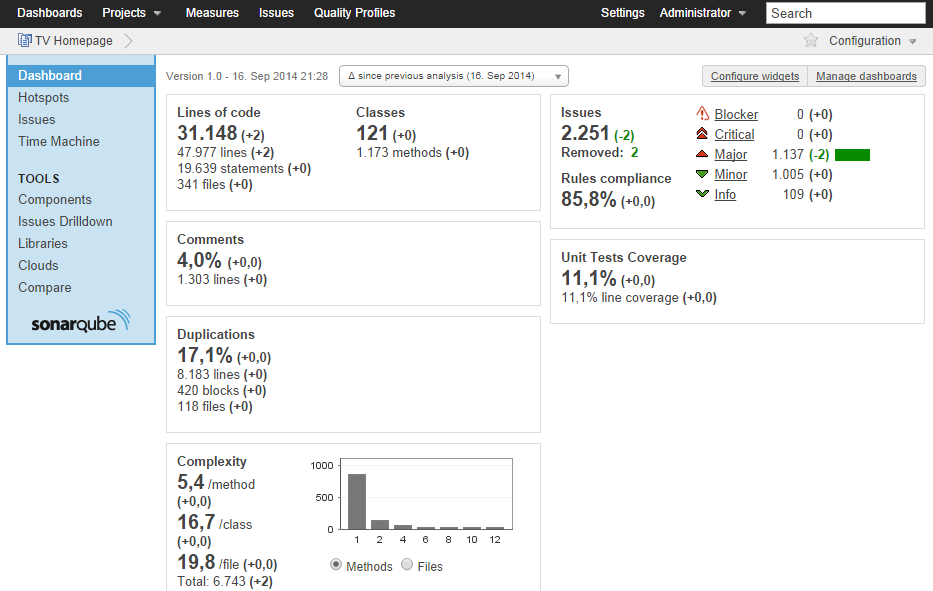
\includegraphics[scale=0.5]{images/sonar_backend.png}
\caption{Sonar - statische Code Analyse Backend}
\label{fig:sonar_backend}
\end{figure}

\begin{figure}[h]
\centering
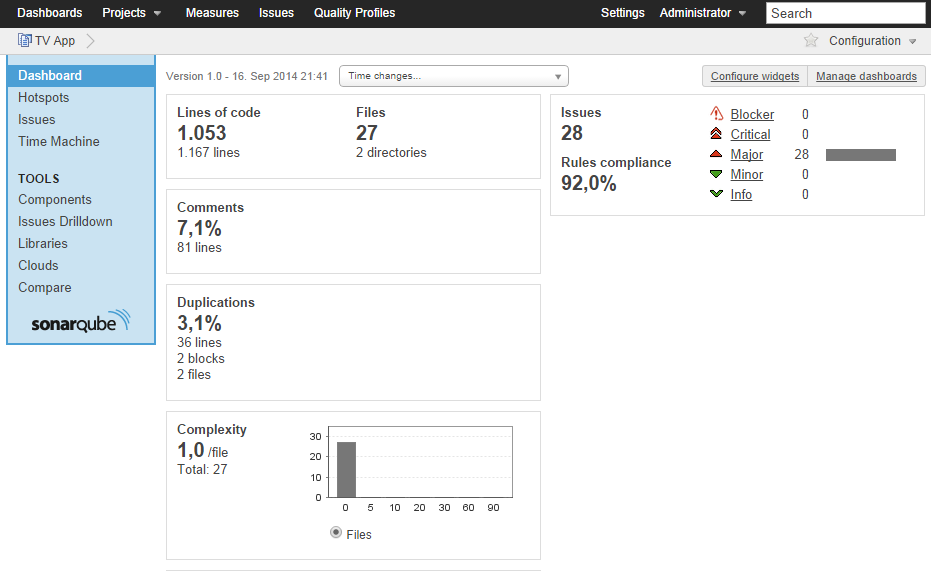
\includegraphics[scale=0.5]{images/sonar_app.png}
\caption{Sonar - statische Code Analyse App}
\label{fig:sonar_app}
\end{figure}

\begin{figure}[h]
\centering
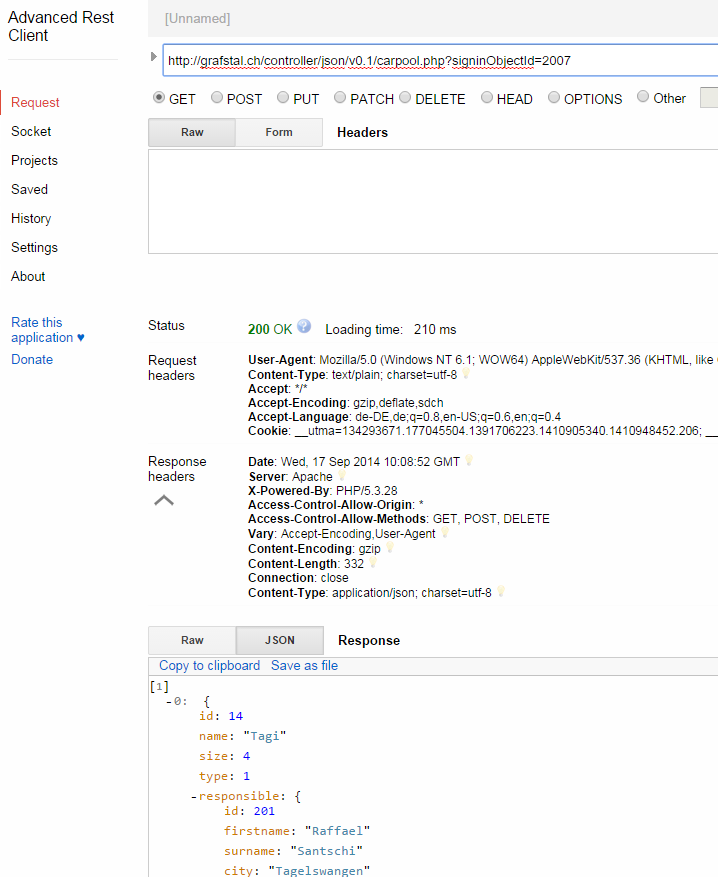
\includegraphics[scale=0.5]{images/advanced_rest_client.png}
\caption{Advanced Rest client}
\label{fig:advanced_rest_client}
\end{figure}

\FloatBarrier


\clearpage
\section{Backend}\label{impl_backend}
In diesem Unterkapitel werden das \glossarmark{Refactoring} des Backends beschrieben und eine Übersicht der Push-Nachricht Implementierung vermittelt.

\subsection{Refactoring}
In diesem Unterkapitel wird kurz der vorgefundene Ist-Zustand beschrieben und danach die Schritte, welche unternommen wurden, um das Backend wartbarer und flexibler zu machen.

\subsubsection{Ist-Zustand}
Am Anfang dieses Projekts war in jeder Klasse HTML- mit \glossarmark{PHP}-Code vermischt und SQL-Abfragen waren überall verstreut. Dies machte es schwierig den Code zu warten. Zusätzlich wurde jede save-, update-, load- und delete-Anweisung von Objekten, wenn es denn solche gab, selber implementiert, was sehr mühsam und unflexibel war. Zudem erweiterten ähnliche Objekte zwar eine Super-Klasse, teilten sich aber keine Tabelle und hatten somit auch verschiedene ID-Sequenzen.\\

Schnell wurde klar, dass man mit diesem Stand kein \glossarmark{API} aufbauen sollte, welches dann von der App angesprochen wird. Um den Code besser zu strukturieren, übersichtlicher und vor allem auch testbar zu machen, wurde ein \glossarmark{Refactoring} (siehe \cite{feathers2004working}) durchgeführt. Ausgehend von der Strategie für das \glossarmark{Refactoring} wurde Doctrine in das Projekt eingebunden. Doctrine ist, wie schon im Kapitel \ref{arch_backend} erklärt, ein \glossarmark{ORM}, welches, richtig eingesetzt, viel Arbeit abnehmen kann. Damit man Doctrine jedoch sinnvoll verwenden konnte, benötigte es zuerst einige Zeit für die Analyse und die Umstellungen.

\subsubsection{Refactoring}
Zuerst wurde geschaut, was zusammengefasst werden konnte. Alle \glossarmark{Entities}, bei denen man sich anmelden kann, wurden ganz getreu dem 'Don’t repeat yourself' Prinzip als SigninObject zusammengefasst, da sie sehr viele gleiche Attribute und Funkionen haben. Im gleichen Zug wurde die Datenbank normalisiert, da zum Teil gleiche Ortsnamen in verschiedenen Tabellen vorhanden waren. Da die einzelnen Typen jedoch auch spezifische Attribute haben, wurde eine Joined-Inheritance (siehe \cite{inheritance_java} und \cite{inheritance_doctrine}) angewendet, welche von vielen \glossarmark{ORMs} unterstützt wird. Die Joined-Inheritance basiert auf einer Grundtabelle, welche alle gemeinsamen Attribute beinhaltet und einer spezifischen Tabelle, welche die anderen Attribute beinhaltet. Die Tabellen werden über eine DiscriminatorColumn miteinander verknüpft. In diesem Konstrukt wurde auch ein Strategy-Pattern (siehe \cite{gof_book}) verwendet, um verschiedene Informationen im Kalender\footnote{Der Kalender (nicht in diesem Projekt entwickelt) kann über ein ics-File auf Geräten eingebunden werden.} anzuzeigen.\\

Dieser Umbau hat den grossen Vorteil, dass für jeden Veranstaltungstyp, sei das ein Training, Match, Sitzung, Anlass oder Helfereinsatz, die gleiche Anmeldefunkion verwendet werden kann. Der Umbau machte sich auch bei der Entwicklung der Fahrgemeinschaftsverwaltung bezahlt, da diese nur ein mal implementiert werden musste.\\

\begin{figure}[h]
\centering
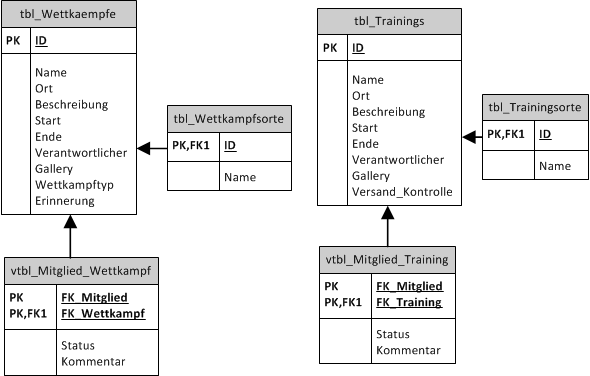
\includegraphics[scale=0.7]{images/visio/datenbankdiagramm_alt.png}
\caption{Datenbankdiagramm alt}
\label{fig:db_schema_alt}
\end{figure}

Das Datenbankdiagramm (siehe Abbildung \ref{fig:db_schema_alt}) zeigt einen kleinen Ausschnitt aus dem Datenbank Schema von früher. Jeder Veranstaltungstyp hatte seine eigene Ortstabelle und seine eigene Verknüpfungstabelle für die Anmeldungen. Wenn man sich nun vorstellt, dass dieses Konstrukt für die fünf verschiedenen Typen vorhanden war, kann man sich denken, wie viele Tabellen schon bereits nur für die Anmeldungen vorhanden waren. Nach dem \glossarmark{Refactoring} sah das Datenbankdiagramm (siehe Abbildung \ref{fig:db_schema_neu}) etwas einfacher aus. Die Orte waren nun in einer Tabelle, die Anmeldungen auch und alle gemeinsamen Attribute wurden in der TerminObjekte-Tabelle gespeichert.

\begin{figure}[h]
\centering
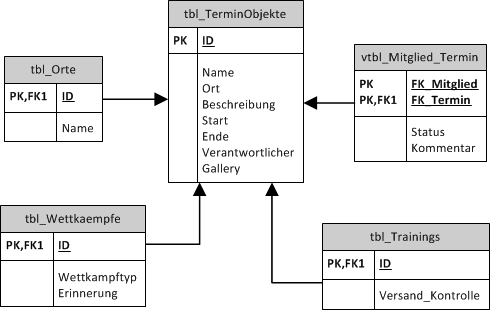
\includegraphics[scale=0.7]{images/visio/datenbankdiagramm_neu.png}
\caption{Datenbankdiagramm neu}
\label{fig:db_schema_neu}
\end{figure}

\FloatBarrier
Durch das \glossarmark{Refactoring} werden weniger SQL-Statements direkt in den Webseiten abgesetzt. Es wird vermehrt\footnote{Nur an Orten, wo die Objekte innerhalb dieses Projektes angefasst wurden} mit Objekten gearbeitet. Ein Repository liefert die gewünschten Objekte zur Webseite, die Abfrage Logik ist somit zentralisiert. Das Repository arbeitet mit einer \glossarmark{Object Query Language} (\glossarmark{OQL}), bei welcher man nicht über die Spalten der Tabelle Werte abfragt, sondern über Attribute des Objekts. Eine Änderung des Spaltennamens hat somit keine grössere Auswirkung als eine kleine Änderung in der \glossarmark{Entity}.\\

Die Struktur sieht nach der Implementierung von Doctrine wie folgt aus:
\begin{itemize}
\item \glossarmark{Entity}: Attribute, Getter und Setter
\item \glossarmark{Entity}-Manager: speichert, löscht und lädt \glossarmark{Entities} oder gibt das Repository der \glossarmark{Entity} zurück
\item Repository: spezifische Abfrage-Logik
\item Services\footnote{Services werden nicht von Doctrine vorgegeben, wurden aber als eine weitere Schicht sogenannte Verarbeitungsschicht implementiert}: Business-Logik
\end{itemize}

\newpage
\subsubsection{Facts and Figures}
Das \glossarmark{Refactoring} war zwar sehr zeitaufwendig, hat jedoch bei einigen Implementationen die Komplexität stark reduziert, Zeitersparnisse eingebracht und wird auch in Zukunft vieles erleichtern.
\begin{itemize}
\item Testabdeckung: Das Testen stellte sich vorher als extrem schwierig heraus und ist nun mit den Kapselungen viel einfacher. Es konnte während des Projekts doch immerhin eine Testabdeckung von 11.1\% erreicht werden. Dieses Resultat wird natürlich noch sehr verfälscht durch Seiten und Funktionen, welche nicht Teil dieses Projekts waren.
\item Duplikate: Der Prozentsatz der duplizierten Linien konnte um fast 6\% reduziert werden, was etwa 4'000 Lines of code bedeutet.
\item Komplexität: Die Komplexität pro Klasse konnte von 40 auf 17 gesenkt werden.
\item Rule compliance: Die Rule compliance konnte um knapp 7\% gesteigert werden.
\item Issues: Über 3000 Issues, darunter alle kritischen und Blocker Issues, konnten behoben werden.
\end{itemize}


\subsection{Push-Nachrichten}
Das Versenden von Push-Nachrichten funktioniert bei iOS und Android ähnlich, jedoch sind die Vorbedingungen sehr unterschiedlich. Bei Android wird ein \glossarmark{API}-Key verwendet, welchen man in der Google Developers Console erstellen kann. Dazu muss man ein Projekt erstellen und 'Google Cloud Messaging for Android' aktivieren. Nun kann man einen neuen \glossarmark{API}-Key erstellen, welcher dann im Backend benötigt wird. Die Projektnummer ist zugleich die Sender ID und wird bei der Registrierung des produktiven Apps über Phonegap benötigt. (siehe dazu \cite{android_push_android} und \cite{devgirl_push_android})\\


Bei iOS ist das etwas anders, als erstes braucht man ein Zertifikat, da nur ein Server mit diesem Zertifikat Push-Nachrichten an den \glossarmark{APNS} senden darf. Es gibt ein Zertifikat für den Entwicklungsserver und ein weiteres für den produktiven Server. Über den Entwicklungsserver können nur verknüpfte\footnote{um die App auf einem Gerät zu testen, muss man es zuerst mit dem Developer Account verknüpfen} Geräte im Entwicklungsmodus erreicht werden. Zusätzlich muss für das Testen der Push-Nachrichten noch ein iOS App Development Provisioning Profile erstellt werden, welches dann auch mit dem Developer Account und den Test Geräten verknüpft wird. Bei der Erstellung der Zertifikate ist es wichtig, dass die App ID mit dem Projekt übereinstimmt, ansonsten kommen die Push-Nachrichten nicht an. Die Registrierung des produktiven Apps über Phonegap ist ganz einfach und nicht projektspezifisch. (siehe dazu \cite{ios_push})\\

Nach der Registrierung des jeweiligen Services schickt die App den Geräteschlüssel mit der Mitglieder ID ans Backend, welches den Schlüssel mit der Verknüpfung zum Mitglied speichert. Nun hat man den Schlüssel, den man für das gezielte Versenden von Push-Nachrichten benötigt.
\begin{figure}[ht]
\centering
\subfigure[Registration]{
  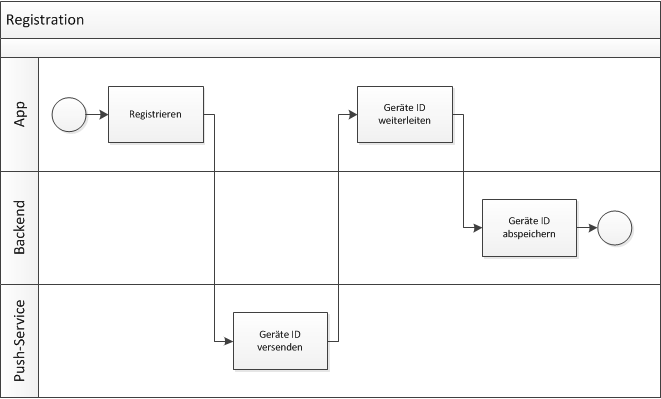
\includegraphics[scale=0.7]{images/visio/push_notification_flow_reg.png}
  \label{fig:push_notification_flow_reg}
}
\subfigure[Mitteilung versenden]{
  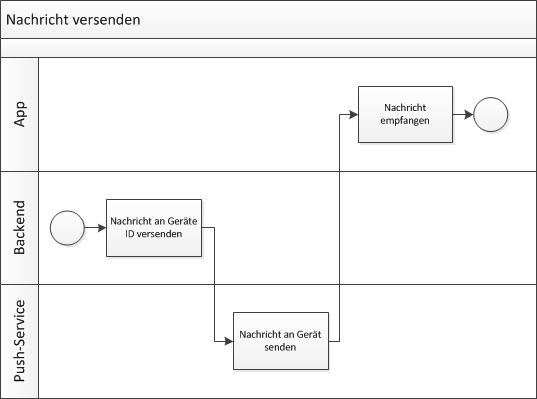
\includegraphics[scale=0.7]{images/visio/push_notification_flow_send.png}
  \label{fig:push_notification_flow_send}
}
\label{fig:app_settings}
\caption{Ablauf von Push-Nachrichten}
\end{figure}

\subsection{Resultierende Quellcode}
Dieses Projekt wurde auf einem bereits bestehenden Backend aufgebaut, alle Änderungen ab der Revision 3c54a42a698abdeee1779c71542786bd6707237b wurden innerhalb dieses Projekt getätigt. Für die Arbeiten im \glossarmark{Refactoring} wurden zwei neue Branches erstellt. Zum einen der 'refactoring' Branch, in welchem die Änderungen für die Datenmigration abgelegt wurden und zum anderen der 'jpa\_implementation' Branch, in welchem das eigentliche \glossarmark{Refactoring} durchgeführt wurde. In diesem Branch wurde gearbeitet bis der Stand produktionsreif war. Der 'jpa\_implementation' Branch wurde dann wieder in den 'master' Branch geführt. In der Projektzeit 


\section{Mobile App}\label{impl_moblie_app}
In diesem Unterkapitel werden neben einem detailierten Aufbau der App, die unterschiedlichen Provisioning Prozesse und die Probleme bei der Umsetzung beschrieben.

\subsection{Aufbau}
Das Menü (siehe Abbildung \ref{fig:navigation}) der App wurde sehr schlicht gehalten und sehr leicht erweiterbar gemacht. Die Einträge News, Vereine und Veranstaltungen sind für alle Benutzer sichtbar, wenn auch mit benutzerspezifischem Inhalt und Design. Der Link zu den Resultaten ist nur für angemeldete Benutzer verfügbar.

\begin{figure}[h]
\centering
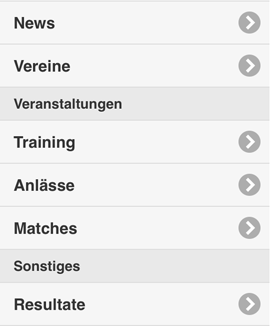
\includegraphics{images/app/navigation.png}
\caption{Navigation im App}
\label{fig:navigation}
\end{figure}

\FloatBarrier
\subsubsection{News}
Die News Seite (siehe Abbildung \ref{fig:app_news}) ist zugleich auch die Startseite, wenn die App aufgemacht wird. Auf ihr werden die neusten drei Berichte angezeigt. Der Aufbau ist wie auf der Homepage, die Elemente enthalten lediglich einen Einleitungstext. Erst wenn man auf das Element klickt kann man den ganzen Bericht lesen. Dies hat den einfachen Grund, dass die Berichte zum Teil sehr lang sind und dann die anderen Berichte verloren gehen. Bei angemeldeten Mitgliedern wird zusätzlich noch die nächste Veranstaltung angezeigt, damit man sich sofort an- bzw. abmelden und wichtige Informationen nachschlagen kann.

\begin{figure}[h]
\centering
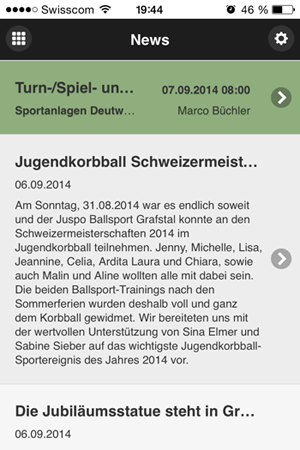
\includegraphics[scale=0.5]{images/app/news.png}
\caption{News Seite}
\label{fig:app_news}
\end{figure}

\FloatBarrier
\subsubsection{Vereine}
Die Vereine Seite (siehe Abbildung \ref{fig:app_vereine})  listet alle Vereine und Riegen der Turner Familie Grafstal auf. Wenn man auf eine Riege klickt, erhält man zusätzliche Informationen, wie zum Beispiel die Trainingszeiten. Diese Seite enthält vor allem Informationen für die Öffentlichkeit oder ist ein Nachschlagewerk für Mitglieder.


\begin{figure}[h]
\centering
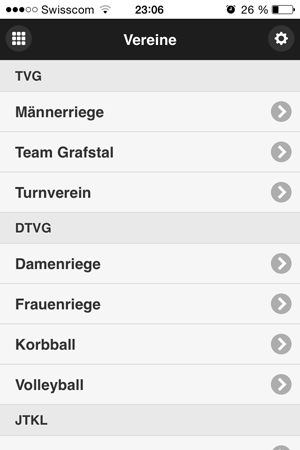
\includegraphics[scale=0.5]{images/app/vereine.png}
\caption{Vereinsseite}
\label{fig:app_vereine}
\end{figure}

\newpage
\FloatBarrier
\subsubsection{Veranstaltungen}
Die drei Veranstaltungsseiten sind alle gleich aufgebaut (siehe Abbildung \ref{fig:app_trainings}), sie zeigen die aktuellen Elemente mit Name, Datum, Zeit, Ort und Verantwortlichen. Falls der Benutzer angemeldet ist, wird durch Farbe angezeigt, ob er sich angemeldet (grün), abgemeldet (rot) oder nichts von beidem (grau) hat.
\begin{figure}[ht]
\centering
\subfigure[Anlässe (nicht angemeldet)]{
  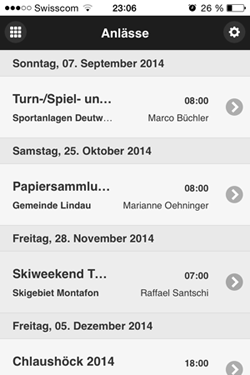
\includegraphics[scale=0.5]{images/app/events.png}
  \label{fig:app_events}
}
\subfigure[Trainings (angemeldet)]{
  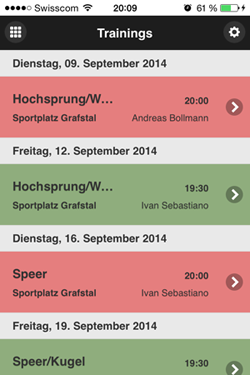
\includegraphics[scale=0.5]{images/app/trainings.png}
  \label{fig:app_trainings}
}
\label{fig:app_singinobjects}
\caption{Veranstaltungen}
\end{figure}

Wenn auf eine Veranstaltung geklickt wird, geht eine Detailansicht (siehe Abbildung \ref{fig:app_detail_event}) auf. In dieser Ansicht erhält man weitere Information, kann sich an- und abmelden und kommt auch zu den Fahrgemeinschaften. Die Information, wer sich angemeldet hat, sehen nur angemeldete Benutzer.

\begin{figure}[h]
\centering
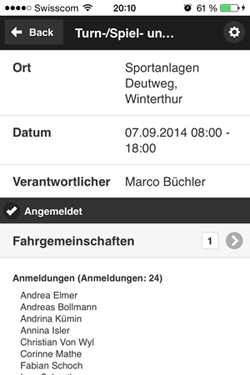
\includegraphics[scale=0.5]{images/app/event_detail.png}
\caption{Anlass Details}
\label{fig:app_detail_event}
\end{figure}

\newpage
\FloatBarrier
\subsubsection{Fahrgemeinschaften}
Bei jeder Veranstaltung können Fahrgemeinschaften erstellt werden, welche dann in der Übersicht (siehe Abbildung \ref{fig:app_carpools}) angezeigt werden. Man sieht den Namen, den Fahrer und dessen Wohnort. Zusätzlich sieht man, wie viele Plätze noch frei sind oder ob man bereits angemeldet ist. In der Detailansicht (siehe Abbildung \ref{fig:app_carpool_detail}) kann man sich anmelden und erhält eine Liste der Mitfahrenden.
\begin{figure}[ht]
\centering
\subfigure[Fahrgemeinschaften]{
  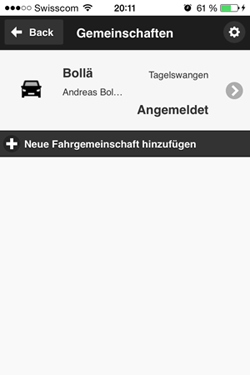
\includegraphics[scale=0.5]{images/app/carpools.png}
  \label{fig:app_carpools}
}
\subfigure[Fahrgemeinschaft Detail]{
  \includegraphics[scale=0.5]{images/app/carpool_detail.png}
  \label{fig:app_carpool_detail}
}
\label{fig:app_carpool_page}
\caption{Veranstaltungen}
\end{figure}

Im Formular (siehe Abbildung \ref{fig:app_add_carpool}) für die Erstellung einer neuen Fahrgemeinschaft muss man einen Namen angeben und kann den Typ der Gemeinschaft wählen, nur wenn es eine 'Car'-Fahrgemeinschaft ist, muss man die freien Plätze angeben.

\begin{figure}[h]
\centering
\includegraphics[scale=0.5]{images/app/add_carpool.png}
\caption{Fahrgemeinschaft erstellen}
\label{fig:app_add_carpool}
\end{figure}


\newpage
\FloatBarrier
\subsubsection{Resultate}
Unter Resultate (siehe Abbildung \ref{fig:app_results}) finden angemeldete Benutzer ihre Bestleistungen und die Resultate für die \glossarmark{Büchsenliste}.
\begin{figure}[h]
\centering
\includegraphics[scale=0.5]{images/app/results.png}
\caption{Resultate Seite}
\label{fig:app_results}
\end{figure}


\FloatBarrier
\subsubsection{Einstellungen}
In den Einstellungen kann sich der Benutzer nicht nur einloggen (siehe Abbildung \ref{fig:app_login}), sondern auch wählen, für welche Riege er die Matches, Anlässe und Trainings sehen möchte (siehe Abbildung \ref{fig:app_riege_setting}). Diese Filter werden dann auf die Veranstaltungsübersichtseiten angewendet.
\begin{figure}[ht]
\centering
\subfigure[Login Formular]{
  \includegraphics[scale=0.5]{images/app/settings1.png}
  \label{fig:app_login}
}
\subfigure[Riegen Einstellungen]{
  \includegraphics[scale=0.5]{images/app/settings2.png}
  \label{fig:app_riege_setting}
}
\label{fig:app_settings}
\caption{Einstellungen}
\end{figure}

\newpage
\FloatBarrier
\subsection{Javascript Funktionen}
Die Javascript Funktionen wurden möglichst generisch gewählt, damit man sie an verschiedenen Orten wiederverwenden kann. Mit diesem Ansatz ist man bei den verschiedenen Veranstaltungsseiten mit wenig Code ausgekommen. Es war auch einfach, die nächste bevorstehende Veranstaltung auf der Startseite gleich anzuzeigen, wie auf den anderen Seiten. Das App kommt durch das mit knapp 2'000 Zeilen Code aus. Die Funktionen wurden in unterschiedliche Files geschrieben, welche nach ihrem Zweck benannt wurden.
\begin{itemize}
\item carpool.js: an- und abmelden bei Fahrgemeinschaften, anzeigen von Fahrgemeinschaften
\item help.js:  Datum formatieren,  Listen-Elemente erstellen, Navigationselemente
\item index.js: initialisieren der Push-Benachrichtigungen
\item news.js: Berichte laden
\item result.js: Resultate anzeigen
\item settings.js: Dropwdowns initialisieren, an- und abmelden, Riegenfilter setzen
\item signinObject.js: Veranstaltungen laden, Veranstaltungsdetails anzeigen, an- und abmelden bei Veranstaltungen 
\end{itemize}

\subsection{Login}
Da das Backend nur über eine HTTP-Verbindung verfügte und die Anmeldedaten nicht im \glossarmark{localStorage}  gespeichert werden sollten, wurde darauf verzichtet, die Anmeldedaten bei jeder Anfrage an das Backend mitzusenden. Bei der Anmeldung wird die Mitglieder-ID gespeichert und bei einer Anfrage mitgeteilt. In einem späteren Projekt sollte diese Lösung durch eine \glossarmark{Session-ID} abgelöst werden.

\subsection{Provisioning Prozesse}
Die Entwicklung der App ist das eine, die Bereitstellung zum Download das andere. Phonegap hilft beim Provisioning vor allem bei Android. Es erstellt, richtig konfiguriert, ein signiertes APK-Paket, welches in der Google Play Developer Console hochgeladen werden kann. Zuerst muss man jedoch einen Developer Account eröffnen. Anschliessend kann man die Beschreibung und die Screenshots für die App hochladen. Das ganze dauert nur wenige Minuten, eine Stunde nach dem Absenden findet man seine App in Google Play. Es empfiehlt sich, die App noch mit eine Absender-ID zu verknüpfen, damit man Statistiken über die Downloadzahlen ansehen kann. (siehe dazu auch \cite{android_prov})

Bei Apple sieht das etwas anders aus: Phonegap kann kein Paket erstellen, es erstellt lediglich das Projekt. Das Projekt muss man dann in XCode öffnen und von dort aus das eigentliche Paket erstellen. Auch hier benötigt man einen Developer Account, den man wahrscheinlich bereits besitzt, da man ihn zum Testen auf realen Geräten benötigt. Zusätzlich muss man ein Distribution Certificate erstellen und in XCode hinzufügen. Danach muss man in iTunes Connect noch einige Angaben zu den Inhalten der App machen. Des Weiteren muss man Review Informationen bereitstellen, dass heisst einen Test Benutzer und Informationen zur Entwicklung angeben. Erst wenn die App erfasst wurde, kann man in XCode ein Archiv erstellen und dieses direkt zu iTunes Connect hochladen. Nun werden schon die ersten Tests durchgeführt, ob zum Beispiel die Versionsnummern übereinstimmen und ob für jedes unterstütze Gerät Screenshots erfasst wurden. Falls dies nicht der Fall ist, wird die App abgelehnt und man muss die Dinge beheben. An diesem Punkt beginnt das Warten - die durchschnittliche Review-Zeit beträgt 8 Tage. (siehe dazu auch \cite{apple_prov_apple} und \cite{apple_prov_ralf})

\subsection{Probleme}
Die Entwicklung für verschiedenen Plattformen war nicht immer einfach. Es kann zwar der gleiche Code verwendet werden, jedoch wird dieser zum Teil anders interpretiert. Bei iOS stellte zum Beispiel die Datum Konvertierung von Daten aus \glossarmark{PHP} in Javascript ein Problem dar Die Daten mussten aufgesplittet werden und in Javascript ein neues Datum Objekt mit den einzelnen Teilen erstellt werden. Des Weiteren wurde unter Android der Löschaufruf für Fahrgemeinschaften gepuffert. Die App zeigte zwar an, dass die Fahrgemeinschaft gelöscht worden sei, doch es wurde nie ein Löschauftrag an das Backend geschickt. Dieser Fehler wurde bei jQuery raportiert (siehe \cite{bug_jquery}) und mittels eines Workarounds umgangen. Ein weiterer Fehler (siehe \cite{bug_jquery_mobile}) wurde in jQuery Mobile gefunden, es gab hier Probleme mit der Navigation, wenn die grafischen Übergange von jQuery Mobile abgeschaltet wurden. Dieser Fehler konnte jedoch auch mit einem Workaround umgangen werden.

%%%%%%%%%%%%%%%%%%%%%%%%%%%%%%%%%%%%%%%%%%%%%%%%%%%%%%%%%%%%%%%%%
%
% Project     : Turnverein App
% Title       : 
% File        : tests.tex Rev. 00
% Date        : 07.07.14
% Author      : Raffael Santschi
%
%%%%%%%%%%%%%%%%%%%%%%%%%%%%%%%%%%%%%%%%%%%%%%%%%%%%%%%%%%%%%%%%%

\chapter{Tests}\label{chap.tests} 
In diesem Kapitel wird auf die verschiedenen Tests und Varianten, welche in diesem Projekt verwendet wurden, eingegangen.

\section{Einführung}
In diesem Projekt hat man die sieben Grundsätze aus \cite{test_soft_book} als Leitlinie beim Testen genommen:
\begin{enumerate}
\item \textbf{Testen zeigt die Anwesenheit von Fehlern}: Testabdeckung mit Sonar ermittelt und Anforderungen überprüft
\item \textbf{Vollständiges Testen ist nicht möglich}: Es wurde solange getestet bis die Fehlerfindungsrate einen bestimmte Punkt unterschritten hatte
\item \textbf{Mit dem Testen frühzeitig beginnen}: Die Tests für die neuen Funktionen wurden zur gleichen Zeit wie der Code, geschrieben
\item \textbf{Häufung von Fehlern}: Wenn Fehler auftraten, dann wurde diese Komponente nach der Behebung nochmals intensiv getestet
\item \textbf{Zunehmende Testresistenz (Pesticide paradox)}: Als Änderungen am Code gemacht wurden, wurden die Tests erweitert bzw. angepasst
\item \textbf{Testen ist abhängig vom Umfeld}: Dieses System ist nicht so sicherheitskritisch, wie etwa Systeme im Bank Umfeld, die Dienste werden jedoch rege benutzt, somit sollte die Testintensität in einem normalen Rahmen liegen.
\item \textbf{Trugschluss: Keine Fehler bedeutet eine brauchbares System}: Die Stakeholder wurden schon bei der Mock-up Erstellung mit einbezogen und bekamen auch während der Entwicklung immer wieder einen Blick in den aktuellen Stand.
\end{enumerate}

\section{Testing}
Komponententests und Integrationstests wurden im Backend mit PHPUnit durchgeführt. Bei den Integrationstests wurde eine In-Memory Datenbank verwendet, welche bei jedem Testlauf neu geladen wird, somit ist man komplett unabhängig von äusseren Einflüssen. Die Testabdeckung wurde mit Sonar überprüft, hier wurde vor allem ein Augenmerk auf die neuen Funktionen und in diesem Projekt verwendete Funktionen gelegt. Neben den verschiedenen Entitäten wurden die Repositories und die Services getestet. (siehe \cite{test_soft_book})

\subsection{Testphasen}
Es wurde festgelegt, dass das Projekt nicht mit der Implementation fertig ist, sondern mit der definitiven Auslieferung. Damit der Kunde genug Erfahrungen sammeln kann, wurden Testphasen definiert. Erst nach Beendigung dieser Testphasen, konnte das Produkt abgenommen werden. Die Testphasen wurden getrennt, damit Fehler klar abgegrenzt werden konnten und für die Behandlung der gemeldeten Fehler auch mehr Zeit zur Verfügung stand.

\subsubsection{Backend}
Die Testphase des Backends begann nach dem lokalen Testing des Refactorings und der Produktiv Schaltung des Backends. Die Mitglieder wurden informiert, dass sie theoretisch keine grossen Änderungen feststellen sollten und sie sollten sich doch bitte bei negativen Abweichungen zur vorherigen Version sofort melden. Es wurden nur wenige Spezialfälle gemeldet, welche schnell behoben werden konnten.

\subsubsection{App}
Da die Freigabe der iOS App mehrere Tage benötigt, wurde die erste Testphase auf Android gemacht. So konnte schneller Feedback eingeholt werden. Die App wurde hochgeladen und nur wenige Personen wurden informiert. Nach wenigen Stunden gab es bereits über 10 Downloads. Das Feedback war gut, lediglich einige kleine Fehler wurden gefunden. Alle Fehler wurden behoben und ein paar kleine Verbesserungsvorschläge umgesetzt, getestet und dann in einer neuen Version hochgeladen. Grössere Anforderungen wurden erfasst, deren Umsetzung jedoch auf kommende Versionen verschoben. Als keine negativen Rückmeldungen mehr kamen und auch beim Nachfragen nichts mehr zum Vorschein kam, wurde die Testphase mit dem Hochladen der iOS App beendet.

\section{System- und Abnahmetest}
Nach erfolgreichem Testing und Abschluss der Testphasen wurde für den Abnahmetest ein Testprotokoll erstellt, welches vorgängig im Systemtest schon durchgegangen wurde. Das Testprotokoll wurde danach dem Kunden übergeben und von diesem selber nochmals abgearbeitet.

\subsection{Testprotokoll}
Das Testprotokoll basiert auf den Use Cases (siehe \ref{use_cases}) und den Anforderungen (siehe \ref{anforderungen}). Akzeptanz Kriterien mit UND- oder ODER-Verknüpfung wurden aufgesplittet, um sicher zu gehen, dass beide Bedingungen erfüllt sind.

%%\begin{longtable}{ l | p{7cm} | l | l }
\begin{longtable}{>{\raggedright}m{1cm}m{7cm}m{3cm}m{2cm}}

\caption[Testprotokoll]{\label{table:tests}Testprotokoll}\\ 
\toprule
\textbf{ID}&\textbf{Test}&\textbf{Herkunft}&\textbf{erfüllt / nicht erfüllt}\\ \midrule\addlinespace
\endfirsthead
\caption*{\textbf{Tabelle~\ref{table:tests} (Fortsetzung):} Testprotokoll}\\ \toprule
\textbf{ID}&\textbf{Test}&\textbf{Herkunft}&\textbf{erfüllt / nicht erfüllt}\\ \midrule\addlinespace
\endhead

\bottomrule\multicolumn{2}{>{\small\raggedleft\arraybackslash}r}{\slshape Fortsetzung auf der nächsten Seite}\\
\endfoot
\bottomrule
\endlastfoot	

	\addlinespace
	1a	&	Bei bekanntem Username und Password muss es dem Mitglied möglich sein, sich beim Backend anzumelden			
				&	\nameref{table:req_1} 	&	erfüllt\\ \addlinespace\hline \addlinespace
	1b	&	Nach erfolgreichem Anmelden muss es dem Mitglied möglich sein erweiterte Möglichkeiten und Informationen zu erhalten.
				&	\nameref{table:req_1} 	&	erfüllt\\ \addlinespace\hline \addlinespace
	2a	&	Falls ein unbekannter Username eingegeben wurde kommt eine entsprechende Fehlermeldung.			
				&	\nameref{table:req_1} 	&	erfüllt\\ \addlinespace\hline \addlinespace
	2b	&	Falls ein falsches Passwort eingegeben wurde kommt eine entsprechende Fehlermeldung.			
				&	\nameref{table:req_1} 	&	erfüllt\\ \addlinespace\hline \addlinespace
	3	&	Das angemeldete Mitglied kann eine Fahrgemeinschaft eröffnen.		
				&	\nameref{table:req_2} 	&	erfüllt\\ \addlinespace\hline \addlinespace
	4a	&	Bei ungültigen Informationen kommt eine entsprechende Fehlermeldung
				&	\nameref{table:req_2} 	&	erfüllt\\ \addlinespace\hline \addlinespace
	4b	&	Bei nicht ausreichenden Informationen kommt eine entsprechende Fehlermeldung
				&	\nameref{table:req_2} 	&	erfüllt\\ \addlinespace\hline \addlinespace
	5	&	Das angemeldete Mitglied kann die Fahrgemeinschaften anzeigen lassen
				&	\nameref{table:req_3} 	&	erfüllt\\ \addlinespace\hline \addlinespace
	6	&	Das angemeldete Mitglied sieht einen Hinweis, falls es keine Fahrgemeinschaften gibt
				&	\nameref{table:req_3} 	&	erfüllt\\ \addlinespace\hline \addlinespace
	7	&	Das angemeldete Mitglied kann einer Fahrgemeinschaft beitreten
				&	\nameref{table:req_4} 	&	erfüllt\\ \addlinespace\hline \addlinespace
	8	&	Das angemeldete Mitglied kann einer Fahrgemeinschaft nicht erneut beitreten
				&	\nameref{table:req_4} 	&	erfüllt\\ \addlinespace\hline \addlinespace
	9	&	Das angemeldete Mitglied erhält eine Fehlermeldung falls die Fahrgemeinschaft keine Kapazität mehr aufweist
				&	\nameref{table:req_4} 	&	erfüllt\\ \addlinespace\hline \addlinespace
	10	&	Das angemeldete Mitglied kann sich für einen Anlass anmelden
				&	\nameref{table:req_5} 	&	erfüllt\\ \addlinespace\hline \addlinespace
	11	&	Das angemeldete Mitglied kann sich für einen Anlass nicht erneut anmelden
				&	\nameref{table:req_5} 	&	erfüllt\\ \addlinespace\hline \addlinespace
	12	&	Der Benutzer erhält informationen über den ausgewählten Anlass
				&	\nameref{table:req_6} 	&	erfüllt\\ \addlinespace\hline \addlinespace
	13	&	Der Benutzer sieht einen Hinweis, falls keine Anlässe vorhanden sind
				&	\nameref{table:req_6} 	&	erfüllt\\ \addlinespace\hline \addlinespace
	14	&	Das angemeldete Mitglied sieht die erweiterten Informationen zum Anlass
				&	\nameref{table:req_7} 	&	erfüllt\\ \addlinespace\hline \addlinespace
	15	&	Nicht angemeldete Mitglieder sehen die erweiterten Informationen zum Anlass nicht
				&	\nameref{table:req_7} 	&	erfüllt\\ \addlinespace\hline \addlinespace
	16a	&	Der Benutzer erhält Informationen über die verschiedenen Vereine
				&	\nameref{table:req_8} 	&	erfüllt\\ \addlinespace\hline \addlinespace
	16b	&	Der Benutzer erhält Informationen über die verschiedenen Riegen
				&	\nameref{table:req_8} 	&	erfüllt\\ \addlinespace\hline \addlinespace
	17	&	Der Benutzer kann die aktuellen Berichte lesen
				&	\nameref{table:req_9} 	&	erfüllt\\ \addlinespace\hline \addlinespace
	18	&	Das angemeldete Mitglied erhält die Push-Nachrichten
				&	\nameref{table:req_10} 	&	erfüllt\\ \addlinespace\hline \addlinespace
	19a	&	Ein Nutzer mit einem Android Mobiltelefon kann die App öffnen
				&	\nameref{table:req_nf_1} 	&	erfüllt\\ \addlinespace\hline \addlinespace
	19b	&	Ein Nutzer mit einem Android Mobiltelefon kann die App verwenden
				&	\nameref{table:req_nf_1} 	&	erfüllt\\ \addlinespace\hline \addlinespace
	20a	&	Ein Nutzer mit einem iPhone kann die App öffnen
				&	\nameref{table:req_nf_2} 	&	erfüllt\\ \addlinespace\hline \addlinespace
	20b	&	Ein Nutzer mit einem iPhone kann die App verwenden
				&	\nameref{table:req_nf_2} 	&	erfüllt\\ \addlinespace\hline \addlinespace
	21	&	Das System zeigt 'keine Internetverbindung vorhanden' an
				&	Use Case UC-1, UC-2, UC-4, UC-5
										&	erfüllt

\end{longtable}

\section{Abnahme Protokoll}
Nach dem erfolgreichen Abnahmetest wurde vom Kunden das Abnahme Protokoll unterzeichnet (siehe Anhang \ref{anhang_abnahmeprotokoll}).

%%%%%%%%%%%%%%%%%%%%%%%%%%%%%%%%%%%%%%%%%%%%%%%%%%%%%%%%%%%%%%%%%
%
% Project     : Turnverein App
% Title       : 
% File        : fazit.tex Rev. 00
% Date        : 07.07.14
% Author      : Raffael Santschi
%
%%%%%%%%%%%%%%%%%%%%%%%%%%%%%%%%%%%%%%%%%%%%%%%%%%%%%%%%%%%%%%%%%

\chapter{Schlussfolgerungen}\label{chap.Schlussfolgerungen}
In der Schlussfolderung wird kurz auf die Verwendung des Produktes, das Fazit des Erfassers und den Ausblick eingegangen.

\section{Verwendung}\label{fazit_verwendung}
Das App fand schnell grossen Anklang, die Neuigkeit über das App verbreitete sich automatisch. Die Turnvereine machten die Öffentlichkeit zusätzlich über Facebook und ihre Homepage auf das App aufmerksam. Eine Woche nach der Bekanntmachung hatten bereits 50 Personen das App heruntergeladen. Die Fahrgemeinschaftsverwaltung wird benutzt und die Anmeldungen an Veranstaltungen werden vermehrt über das App gemacht.

\section{Fazit}\label{fazit}

Die Entwicklung einer App hat sehr viel Spass gemacht und die Zeit verging wie im Flug. Ich fand es toll, das angeignete Wissen über die Anforderungsanalyse und Architektur einsetzen zu können. Die klar definierten Anforderungen haben mir bei der Entwicklung geholfen und liesen nicht viel Spielraum für Missverständnisse. Die enge Zusammenarbeit mit den Mitgliedern war mir bei der Implementation ebenfalls eine grosse Hilfe.\\

Phonegap ist ein gutes Framework, welches einem viel Arbeit abnimmt und in diesem Projekt die richtige Entscheidung war. Ein App mit Phonegap zu entwicklen, lohnt sich bereits ab zwei Plattformen, da der Wartungsaufwand sonst enorm gross wird. Ich fand es auch toll, dass es auf HTML und Javascript basiert, was mir den Einstieg erleichterte. jQuery Mobile ist zwar mächtig, aber nur so lange man die Standardelemente und Funktionen verwendet, sonst kann es sehr schnell in viel Arbeit ausarten. Die Wahl, jQuery zu verwenden, war eine gute und effiziente Lösung für diesen Prototypen, ich werde mir jedoch überlegen, ob ich in Zukunft vielleicht nicht auf ein flexibleres Framework wechseln möchte.\\

Das Refactoring war in diesem Projekt dringend nötig, hat jedoch auch viel mehr Zeit gekostet als geplant. Ich wünschte mir für spätere Projekte, dass ich bereits Tests vorfinde, was den Umbau einiges einfacher gemacht hätte. Es war spannend eine grössere Datenbankmigration auf produktiven Daten zu planen und dann auch durchzuführen. Mit der neuen Testumgebung und dem ORM machte das Entwickeln richtig Spass.\\

\section{Ausblick}\label{fazit_ausblick}
Ich werde in einem weiteren Schritt wahrscheinlich das App mit Angular JS erweitern. Es sind bereits viele neue Anforderungen von den Mitgliedern eingetroffen, welche in den kommenden Monaten umgesetzt werden. Das positiven Feedback der Mitglieder haben mich sehr gefreut und auch motiviert. Die App ist für den Turnverein, zu mindest für die jüngere Generation, ein voller Erfolg und so soll es auch sein. Zum Schluss kann ich nur noch sagen, es ist ein tolles Gefühl seine eigene App im App Store zu sehen!


\chapter{Verzeichnisse}\label{chap.verzeichnisse}
% %%%%%%%%%%%%%%%%%%%%%%%%%%%%%%%%%%%%%%%%%%%%%%%%%%%%%%%%%%%%%%%%%
%  _____   ____  _____                                          %
% |_   _| /  __||  __ \    Institute of Computitional Physics   %
%   | |  |  /   | |__) |   Zuercher Hochschule Winterthur       %
%   | |  | (    |  ___/    (University of Applied Sciences)     %
%  _| |_ |  \__ | |        8401 Winterthur, Switzerland         %
% |_____| \____||_|                                             %
%%%%%%%%%%%%%%%%%%%%%%%%%%%%%%%%%%%%%%%%%%%%%%%%%%%%%%%%%%%%%%%%%
%
% Project     : LaTeX doc Vorlage für Windows ProTeXt mit TexMakerX
% Title       : 
% File        : literatur.tex Rev. 00
% Date        : 23.4.12
% Author      : Remo Ritzmann
% Feedback bitte an Email: remo.ritzmann@pfunzle.ch
%
%%%%%%%%%%%%%%%%%%%%%%%%%%%%%%%%%%%%%%%%%%%%%%%%%%%%%%%%%%%%%%%%%

Um ein automatisches Literaturverzeichnis mit der 
\href{http://www.zhaw.ch/de/zhaw/hochschulbibliothek/dienstleistungen/literaturverwaltung.html}{ZHAW Literaturverwaltung} oder \href{www.bit.ly/literaturverwaltung}{www.bit.ly/literaturverwaltung} zu erstellen, besuchen Sie die Seite \href{www.refworks.com/refworks}{www.refworks.com/refworks} und erstellen Sie ein neuer Account.

-> \textbf{Für ein neues Konto registrieren}

Bibliographi erstellen -> BibTeX auswählen

%In Einstellungen direkt zu BibTex
%http://scholar.google.ch/scholar_settings?hl=de&as_sdt=0,5



\begin{thebibliography}{99}
\addcontentsline{toc}{section}{Literaturverzeichnis}\label{cha:literaturverzeichnis}

% How to make a Literaturlist nach www.ieee.org/documents/ieeecitationref.pdf
% Erklärung







%Books
\bibitem{robotvision} B. Klaus and P. Horn, Robot Vision. Cambridge, MA: MIT Press, 1986.
%Einzelne Seiten aus Buch
\bibitem{randompatterns} L. Stein, ">Random patterns,"> in Computers and You, J. S. Brake, Ed. New York: Wiley, 1994, pp. 55-70.





%Reports

% Peridicals (Zeitschriften)



% Gibt es eine automatische Konvertierung von Bibtech to LaTeX?

% Alte Beispiele
\bibitem{miktex} Latex Programmiere Umgebung (basic-miktex-2.8.3582.exe)\\
\href{http://www.miktex.org/about}{miktex.org}, 28.03.2010

\bibitem{wireshark}Wireshark, Programm zur Darstellung von Ehternet Packeten\\
\href{http://www.wireshark.org/download.html}{http://www.wireshark.org/download.html}



\end{thebibliography}

\addcontentsline{toc}{section}{Literaturverzeichnis}\label{cha:literaturverzeichnis}
 \bibliography{BibTeX-Literaturverzeichnis/literatur}
 \listoffigures
 \addcontentsline{toc}{section}{Abbildungsverzeichnis}
 \listoftables
 \addcontentsline{toc}{section}{Tabellenverzeichnis}
% \addcontentsline{toc}{chapter}{Symbolverzeichnis}
 %%%%%%%%%%%%%%%%%%%%%%%%%%%%%%%%%%%%%%%%%%%%%%%%%%%%%%%%%%%%%%%%%
%  _____   ____  _____                                          %
% |_   _| /  __||  __ \    Institute of Computitional Physics   %
%   | |  |  /   | |__) |   Zuercher Hochschule Winterthur       %
%   | |  | (    |  ___/    (University of Applied Sciences)     %
%  _| |_ |  \__ | |        8401 Winterthur, Switzerland         %
% |_____| \____||_|                                             %
%%%%%%%%%%%%%%%%%%%%%%%%%%%%%%%%%%%%%%%%%%%%%%%%%%%%%%%%%%%%%%%%%
%
% Project     : LaTeX doc Vorlage für Windows ProTeXt mit TexMakerX
% Title       : 
% File        : glossar.tex Rev. 00
% Date        : 23.4.12
% Author      : Remo Ritzmann
% Feedback bitte an Email: remo.ritzmann@pfunzle.ch
%
%%%%%%%%%%%%%%%%%%%%%%%%%%%%%%%%%%%%%%%%%%%%%%%%%%%%%%%%%%%%%%%%%

\chapter*{Glossar}\label{chap.glossar}
\addcontentsline{toc}{section}{Glossar}\label{cha:glossar}

In diesem Abschnitt werden Abkürzungen und Begriffe kurz erklärt.

\begin{longtable}{|m{3cm}|m{11cm}|}\hline	
	\rowcolor{gray} \textbf{Abk}&
	Abkürzung \\ \hline		


	\textbf{Ajax}&
	(siehe Asynchronous JavaScript and XML)\\ \hline	

	\textbf{Asynchronous JavaScript and XML}&
	Ajax ... bezeichnet ein Konzept der asynchronen Datenübertragung zwischen einem Browser und dem Server. Dieses ermöglicht es, HTTP-Anfragen durchzuführen, während eine HTML-Seite angezeigt wird, und die Seite zu verändern, ohne sie komplett neu zu laden.\cite{wiki_ajax}\\ \hline	

	\textbf{Basisfaktor}&
	Basisfaktoren (unterbewusste Anforderungen) muss das System in jedem Fall vollständig erfüllen, sonst stellt sich beim Stakeholder massive Unzufriedenheit ein. \cite{req_eng_book}\\ \hline	

	\textbf{Begeisterungsfaktor}&
	Begeisterungsfaktoren (unbewusste Anforderungen) sind Merkmale eines Systems, deren Wert ein Stakeholder erst erkennt, wenn er sie selbst ausprobieren kann oder sie vom Requirements Engineer vorgeschlagen werden.\cite{req_eng_book}\\ \hline	

	\textbf{Büchsenliste}&
	Die Büchsenliste wurde vom Turnverein eingeführt, um die Mitgliedern anzuspornen. Ziel ist es bei jedem Wettkampf mindestens gleich gut, wie im letzten Wettkampf zu sein. In der Liste werden die letzten Resultate aufgeführt, damit man weiss, was das minimale Ziel ist. Falls ein Mitglied ein schlechteres Resultat erzielt, muss er einen vordefinierten Betrag in die Büchse (daher der Name) zahlen.\\ \hline	

	\textbf{Entity}&
	Entity (auch Entität) ist ein eindeutig zu bestimmendes Daten-Objekt \\ \hline	

	\textbf{Integrated Development Environment}&
	Eine integrierte Entwicklerumgebung (englisch Integrated Development Environment) beinhalten einen Texteditor, Compiler (falls dieser benötigt wird), Debugger, Formatierungsfunktionen und in dem Kontext der Appentwicklung die Möglichkeit der Erstellung von grafischen Benutzeroberflächen.\\ \hline

	\textbf{IDE}&
	(siehe Integrated Development Environment)\\ \hline

	\textbf{JavaScript Object Notation}&
	Die JavaScript Object Notation, kurz JSON ..., ist ein kompaktes Datenformat in einer einfach lesbaren Textform zum Zweck des Datenaustauschs zwischen Anwendungen.\cite{wiki_json}\\ \hline

	\textbf{JSON}&
	(siehe JavaScript Object Notation)\\ \hline

	\textbf{localStorage}&
	localStorage ist ein begrenzter Speicherbereich im Document Object Model (DOM), welcher auch nach dem Schliessen des Browsers ausgelesen werden kann\\ \hline	

	\textbf{Mockup}&
	Der aus dem Englischen stammende Begriff Mock-up oder Mockup (auch Maquette) bezeichnet im Deutschen beispielsweise eine Attrappe. Er wird heute aber meist für ein maßstäblich gefertigtes Modell bzw. eine Nachbildung zu Präsentationzwecken benutzt, demgegenüber ist der Prototyp ein funktionsfähiges Modell.\cite{wiki_mockup}\\ \hline	

	\textbf{Objektrelationale Abbildung}&
	Objektrelationale Abbildung (englisch object-relational mapping, ORM) ist eine Technik der Softwareentwicklung, mit der ein in einer objektorientierten Programmiersprache geschriebenes Anwendungsprogramm seine Objekte in einer relationalen Datenbank ablegen kann. Dem Programm erscheint die Datenbank dann als objektorientierte Datenbank, was die Programmierung erleichtert. \cite{wiki_orm}\\ \hline	

	\textbf{Object-relational mapping}&
	(siehe Objektrelationale Abbildung)\\ \hline	

	\textbf{Object Query Language}&
	Object Query Language (OQL) ist stark an SQL angeleht, wobei man nicht mit den Spalten der Tabelle, sondern mit den Attributen des Objekts Abfragen erstellt.\\ \hline	

	\textbf{OQL}&
	(siehe Object Query Language)\\ \hline

	\textbf{ORM}&
	(siehe Object-relational mapping)\\ \hline

	\textbf{PHP}&
	PHP (rekursives Akronym und Backronym für „PHP: Hypertext Preprocessor“, ursprünglich „Personal Home Page Tools“) ist eine Skriptsprache mit einer an C und Perl angelehnten Syntax, die hauptsächlich zur Erstellung dynamischer Webseiten oder Webanwendungen verwendet wird.\cite{wiki_php}\\ \hline	

	\textbf{Projektstrukturplan}&
	Ein Synonym für Work Breakdown Structure (WBS): Eine in der Regel an den Liefergegenständen orientierte Anordnung von Projektelementen, die den Gesamtinhalt und -umfang des Projekts strukturiert und definiert.\cite{proj_mgmt_book}\\ \hline	

	\textbf{Stakeholder}&
	Stakeholder sind für den Requirement Engineer wichtige Quellen zur Identifikation möglicher Anforderungen des Systems.\cite{req_eng_book}\\ \hline		

	\textbf{Session-Token}&
	Eine Session-ID ist eine eindeutige ID, welche bei der Anmeldung generiert wird, sie kann dann zur Authentifizierung verwendet werden. Eine Session-ID ist nur eine gewisse Zeit gültig \\ \hline		

Apple Push Notification Service (APNS) und Google Cloud Messaging for Android (GCM)	


\end{longtable}

% \addcontentsline{toc}{section}{Stichwortverzeichnis}
 \lstlistoflistings
 \addcontentsline{toc}{section}{Listingverzeichnis}
 
%%%%%%%%%%%%%%%%%%%%%%%%%%%%%%%%%%%%%%%%%%%%%%%%%%%%%%%%%%%%%%%%%
%
% Project     : Turnverein App
% Title       : 
% File        : anhang.tex Rev. 00
% Date        : 07.07.14
% Author      : Raffael Santschi
%
%%%%%%%%%%%%%%%%%%%%%%%%%%%%%%%%%%%%%%%%%%%%%%%%%%%%%%%%%%%%%%%%%


\pagenumbering{Roman}

\appendix
\chapter{Anhang}\label{chap.anhang}



\section{Abnahmeprotokoll}\label{anhang_abnahmeprotokoll}
\includepdf{images/word/Abnahmeprotokoll.pdf}


\end{document}
